\chapter{先进绝热压缩空气储能通用宽工况热力学仿真模型}
\label{cha:simulation}

\section{概述}
\label{sec:chap2-intro}

电池储能作为电化学储能中的典型代表,存在着不同种类的变体,如铅酸电池、镍镉电池、锂电池等\cite{Battery-Nature-15, ESS-Review-09}。同样地,AA-CAES也存在多种实现形式,如本文关注的经典AA-CAES储能(第\ref{cha:aa-caes}章)、多能联供型AA-CAES(第\ref{cha:st-caes}章)、风-储集成型AA-CAES(第\ref{cha:ca-recs}章)等。类似于电池储能各变体的基本组件及特性大同小异,AA-CAES各实现形式均包含压缩机、空气透平、换热器、储气库、储热系统等基本组件,深入分析各基本组件的运行特性并建立相应的稳态热力学仿真模型是研究AA-CAES系统级运行特性及调度运行与市场运营方法的前提。

在新能源电力系统应用背景下,AA-CAES各实现形式均不同程度的运行于非额定工况。具体地,若应用于电源侧与风电协同,则压缩机与空气透平将处于部分负载运行;若应用于电网侧削峰填谷及容量备用,AA-CAES将响应价格与负荷波动运行非额定工况;若应用于多能互补系统,AA-CAES内部组件将通过运行于非设计工况响应电热负荷需求的频繁变化。因此,需要分析外部运行环境提出的宽工况运行要求引起的内部组件的部分负载运行特性对AA-CAES整体运行特性的影响。

实现准确的热力学特性建模是分析AA-CAES宽工况运行性能的基本前提。本章提出了计及组件部分负载运行特性的AA-CAES通用宽工况热力学仿真模型,考虑了“常压—常压”、“常压—滑压”、“滑压—常压”、“滑压—滑压”等四种不同的膨胀机与压缩机运行模式;针对容积控制型储气库,建立通用定容、等温、绝热三种储气库模型,进而构建了基于热力学第一定律与热力学第二定律的通用仿真模型,从而为后续章节应用于新能源电力系统源、网、荷侧的不同AA-CAES实现形式的建模与分析奠定基础。

本章结构安排如图~\ref{fig:Model-Flow-Chart}所示,第~\ref{sec:chap2-struc-supply}~节考虑包含各常规组件的典型AA-CAES系统结构,分析其运行模式与供能模式,为研究系统级宽工况热力学仿真模型提供依据;第~\ref{sec:part-load-energy}~ 节基于热力学第一定律,建立~AA-CAES~各组件的部分负载仿真模型及边界条件;第~\ref{sec:chap2-part-load-exergy}~节基于热力学第二定律,建立各组件的宽工况㶲模型;第~\ref{sec:chap2-bound-measure}~节基于构建的热力学仿真模型分析一典型 AA-CAES系统的内部热力学特性及外部供能特性。
%从而为第\ref{cha:aa-caes}章至第\ref{cha:ca-recs}章源—网— 荷三侧典型AA-CAES应用形式的准确建模与运行方法研究提供基础。

\begin{figure}[H] % use float package if you want it here
  \centering
  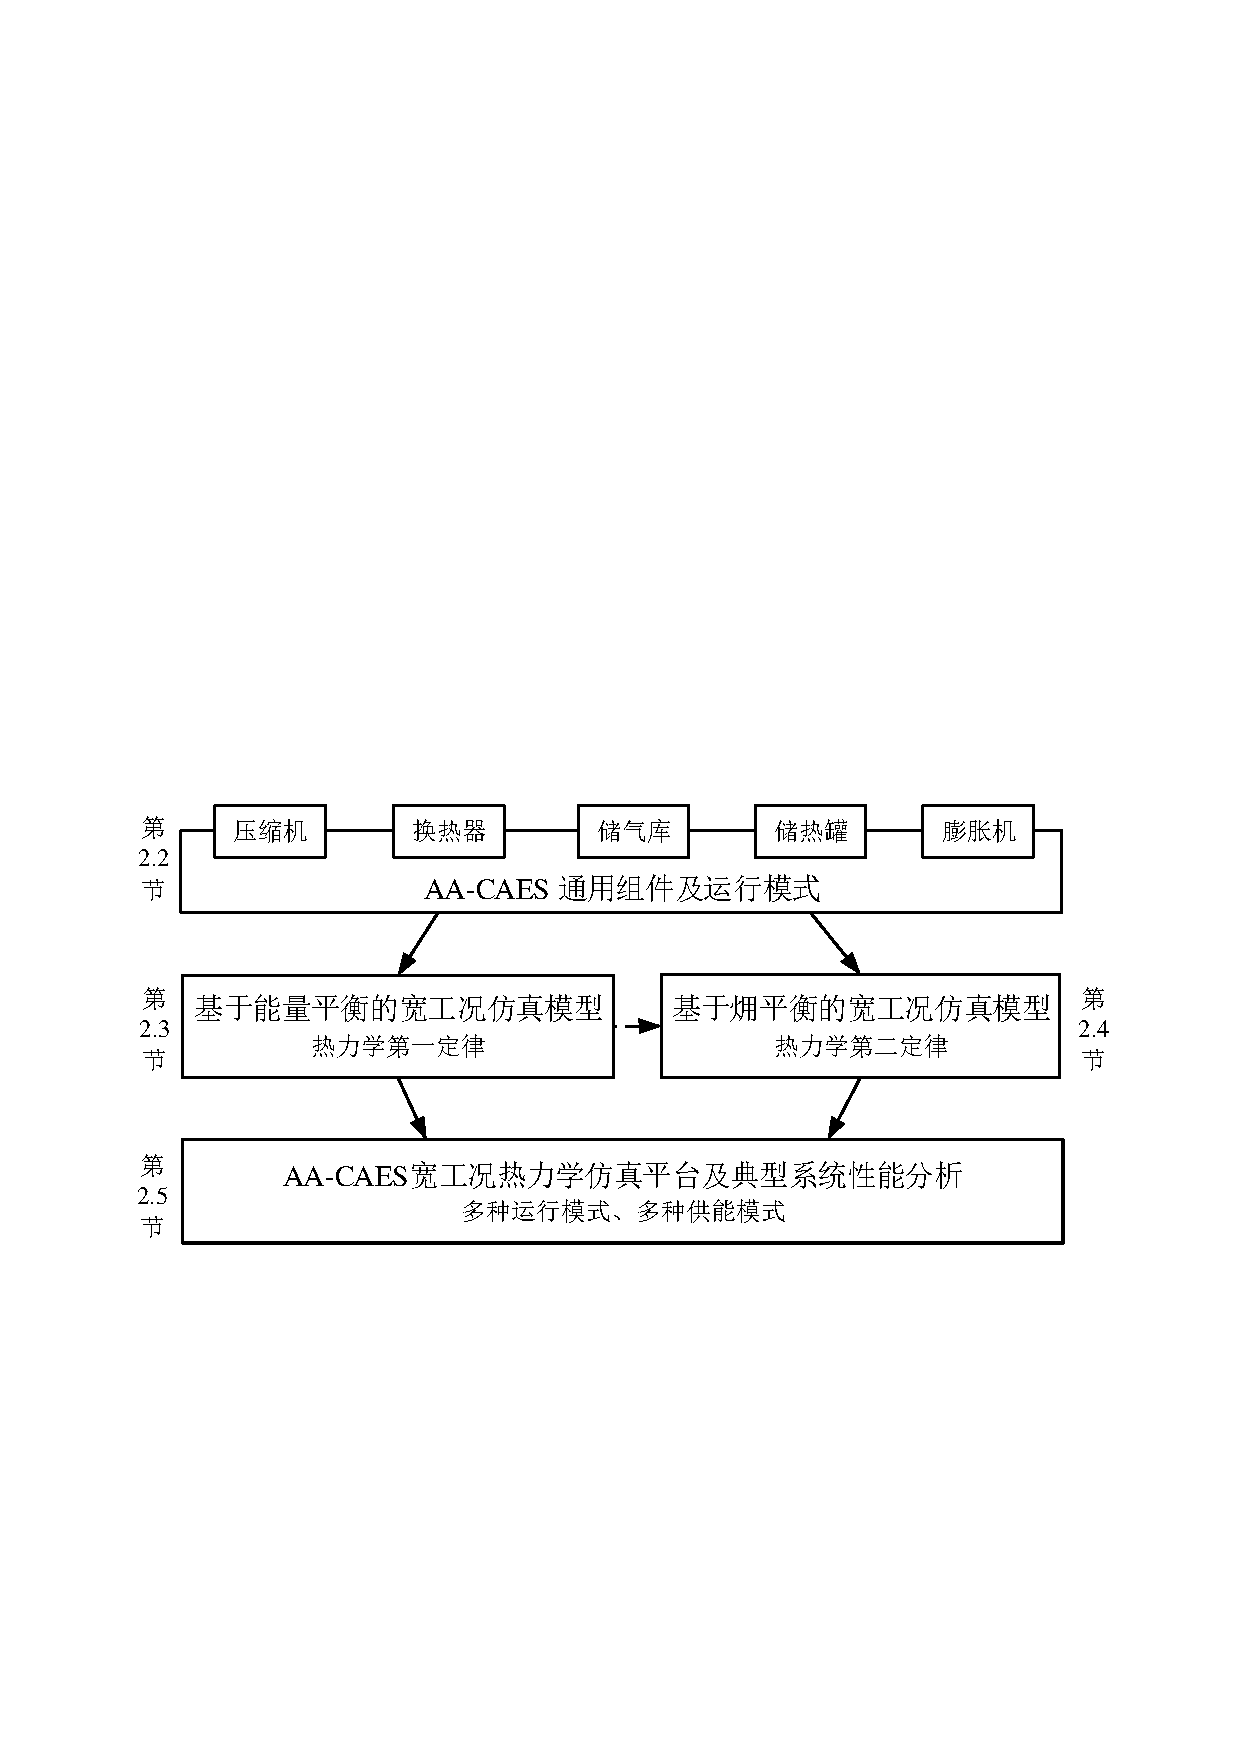
\includegraphics[scale=0.80]{figures/Chap2-1-Model-Flow-Chart-V6.pdf}
  \caption{第2章结构安排}
  \label{fig:Model-Flow-Chart}
\end{figure}

\section{运行模式与供能模式}
\label{sec:chap2-struc-supply}
\subsection{系统结构}
为实现较高的电效率及热利用率,AA-CAES一般采用“多级压缩、级间冷却”与“多级膨胀、级间再热”结构,以逼近“局部准绝热,整体准等温”\cite{Thesis-Zhangxuelin}的热力学流程,如图~\ref{fig:CAES-thermal-struc}所示的典型两级压缩、两级膨胀系统(图中LP与HP分别表示低压级与高压级)。为进一步提高系统的能量利用效率,实际电站(如McIntosh 电站)一般会采用透平乏气(排气)预热透平入口空气。本章重点关注内部组件级的部分负载热力学特性,不考虑采用透平乏气预热空气以提升透平入口空气焓值的做法。

\begin{figure}[H] % use float package if you want it here
  \centering
  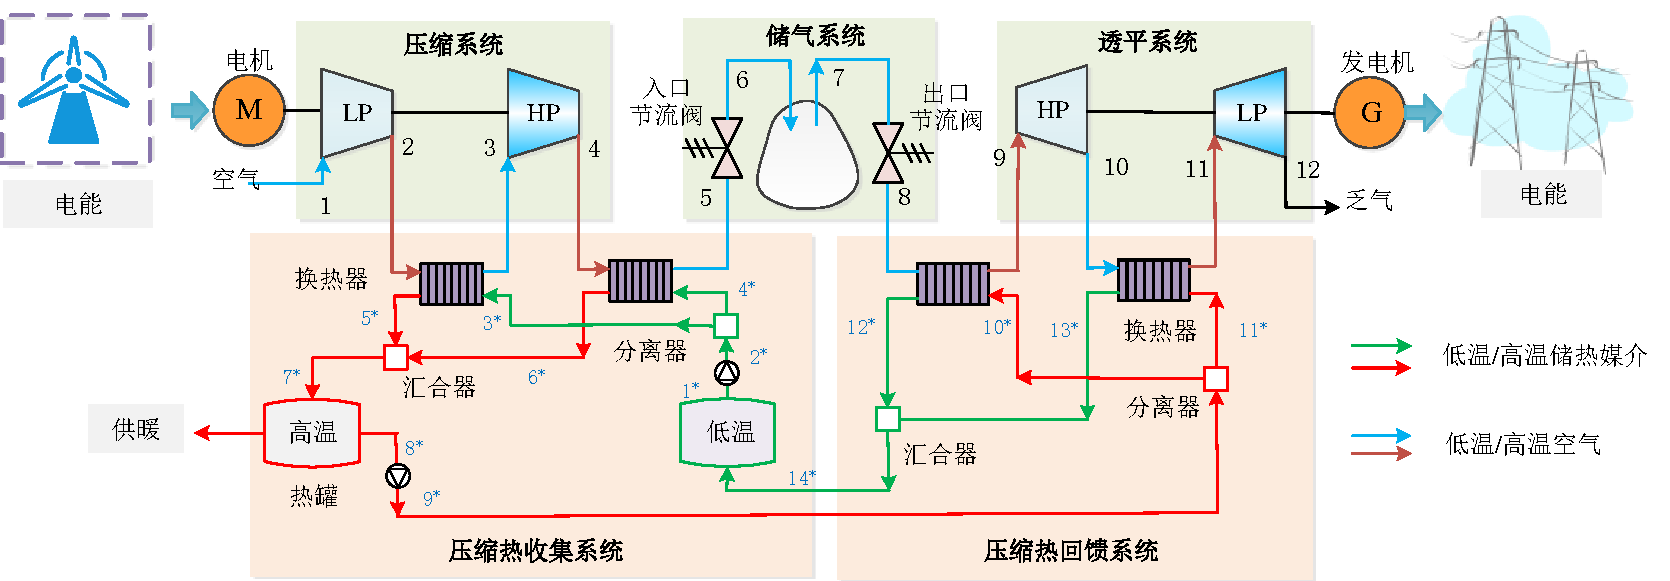
\includegraphics[scale=0.57]{figures/Chap2-1-AA-CAES-Struc-Thermo.pdf}
  \caption{典型AA-CAES结构示意图}
  \label{fig:CAES-thermal-struc}
\end{figure}

为便于分析,除特殊说明外,本章及后续章节AA-CAES各实现形式的热力学特性分析、建模及运行与运营等问题中采用如下假设:
\begin{itemize}
  \item 空气为理想气体, 满足理想气体状态方程;
  \item 空气与传热介质及储热介质的比热容均为常数\footnote{工程热力学中存在更精确的比热容计算方法,如采用首末热力学状态点的平均比热容等,本文不予考虑。};
  \item 不考虑压缩机与电动机、膨胀机与发电机间的能量转换效率(或能量损失);
  \item 忽略压缩热收集与回馈系统中储热介质及载热流体升压泵的耗功;
  \item 不计及载热介质经过泵后引起的温度变化;
  \item 储气库入口及出口的空气节流(若部署相应的节流阀)过程均为绝热过程;
  \item 仅考虑定容储气库模型, 不考虑定压储气库模型;
  \item 不考虑储气库的气体泄漏问题;
  \item 忽略整个过程中工作介质的动量变化及重力势能变化。
  \item 忽略相关管道的热耗散与压力损失。
\end{itemize}

\subsection{运行模式(压力视角)}
根据压缩机背压以及透平入口空气压力的恒定与否,CAES电站可以存在多种运行模式。针对D-CAES电站,文献\inlinecite{CAES-Discharge-16}研究了由储气库出口侧节流阀的控制实现的固定入口空气压力(常压)与变入口空气压力(滑压)等透平运行模式。针对AA-CAES型多能联供系统,文献\inlinecite{CAES-CCHP-off-design-18}引入了由储气库入口与出口节流阀的有无界定的四种运行模式。为实现更加通用的宽工况热力学特性建模,本文引入文献\inlinecite{CAES-Discharge-16,CAES-CCHP-off-design-18}中的运行模式概念。具体地,由末级压缩机出口空气压力与首级膨胀机入口空气压力是否(相对)恒定来界定如下四种运行模式:

(1)常压—常压

 常压—常压运行模式下,图~\ref{fig:CAES-thermal-struc}中入口侧及出口侧的节流阀均处于投入状态。储气库入口侧节流阀的入口空气压力为储气库的最大工作压力,背压为储气库实时压力;出口侧节流阀的入口压力为储气库实时压力,出口压力为储气库的最小工作压力。

(2)常压—滑压

 常压—滑压运行模式下,图~\ref{fig:CAES-thermal-struc}中入口侧节流阀处于投入状态,出口侧节流阀处于停滞状态。储气库入口侧节流阀的入口压力为储气库最大工作压力,背压为储气库实时压力;首级透平的入口空气压力为储气库实时压力,透平处于变压力运行方式。

(3)滑压—常压

滑压—常压运行模式下,图~\ref{fig:CAES-thermal-struc}中储气库入口侧节流阀处于停滞状态,出口侧的节流阀处于投运状态。末级压缩机的出口压力为储气库实时压力,处于变压力运行方式;出口侧节流阀的入口压力为储气库实时压力,出口压力为储气库最小工作压力。

(4)滑压—滑压

滑压—滑压运行模式下,储气库入口侧及出口侧节流阀均处于停滞状态。末级压缩机的出口空气压力与首级透平的进口空气压力均为储气库实时压力,压缩机与膨胀机均处于变压力运行模式。

需要说明的是,通过引入节流阀可以在一定程度上改善压缩机与膨胀机的运行工况,当然也会导致一定的节流损失。然而,上述四种运行模式中通过节流阀维持压缩机和膨胀机的出口与入口空气压力处于额定值的思路仅能改善压缩机和膨胀机受储气库空气压力变化而引起的偏离设计点运行的情形,难以消除AA-CAES因受外部宽工况运行指令导致的压缩机与膨胀机因质量流率等偏离设计点以及储气库中空气与储热系统中储热介质的温度变化等引起的部分负载状态下的低效运行问题。在一定条件下,该问题可通过压缩机与膨胀机的最优转速控制来改善,如文献\inlinecite{ST-CAES-Control-18-CXT}中针对光热复合压缩空气储能系统膨胀机的最优转速控制,以及文献\inlinecite{CA-RECS-Model-Rui-18} 中压缩/膨胀复合机的最优转速控制等。事实上,膨胀机受入口空气温度变化引起的部分负载运行可通过在膨胀机入口与换热器出口间增设电阻丝加热装置等(如文献
\inlinecite{HTH-CAES-Berk-18})进行抑制;本文不考虑该情形,但本文后续的分析方法仅做适当修改即可适用于该类系统。

\subsection{供能模式(温度视角)}
为便于后续章节研究以储能形式应用的AA-CAES电站、以负荷形式应用的AA-CAES能量枢纽,本文假设AA-CAES具有供电模式与热电联供模式等两种供能模式。由于发电机(电动机)电能-机械能(机械能-电能)的转换效率很高,源侧利用AA-CAES的机械输入与输出接口的过程中去除(压缩机前的)电动机与(膨胀机后的)发电机时的供能模式可视为供电模式的特例。

(1)供电模式

 在供电模式下,AA-CAES透平侧需要的入口空气温度较高,往往需反馈全部压缩热,或同时辅助末级透平乏气预热首级透平进口温度。此时,压缩阶段收集的压缩热可富余的供热量较少,AA-CAES 主要应用于电力系统电能单能流应用场景。该模式是面向电力系统的AA-CAES储能电站的主要供能模式,在该模式下AA-CAES储能电站可参与电量市场及辅助服务市场进行运营。

(2)热电联供模式

在热电联供模式下,压缩阶段收集的压缩热能可部分用于供热,存在压缩-供热、静置-供热及膨胀-供热等情形。此时,回馈给透平发电阶段的压缩热较少,透平的入口空气温度较低,从而导致透平排气温度较低,具备制冷能力。该模式主要应用于面向分布式多能互补系统或区域综合能源系统中的AA-CAES型能量枢纽。正如第
\ref{sec:flexibility-poly-generation}节分析,在热电联供模式下一般需要辅助其它(外部)热源,以提高能量枢纽的热电联供能力。

%\subsection{热力学特性与系统效率}
%分析AA-CAES内部组件的功–能转换特性与动态特性,揭示空气压缩热能与空气压力势能间的能流耦合机理,探寻能效提升措施,进而设计面向源-网-荷侧不同应用场景的结构形式,是充分挖掘可再生能源系统中AA-CAES的常规灵活性、供能灵活性及接口灵活性的前提。效率是AA-CAES应用研究中最为关心的问题之一,是制约CAES技术推广应用的瓶颈。一般而言,AA-CAES的效率可从额定工况点效率与宽工况运行效率两个方面进行考察\cite{CAES-Review-18-Rui-operation}。

%\subsubsection{额定工况效率}
%与电池储能、抽水蓄能等技术的循环效率评估方式不同,AA-CAES 效率评估具有其独特的多能流输入及多能流输出特性,具体表现在因富余压缩热能、透平乏气或外部光热热源供热赋予的热能、电能联供能力,使得AA-CAES具备了多能流(输入)输出特性。为此,本文重点关注AA-CAES在仅供电模式下的电–电转换效率与多能联供模式下的能量综合利用效率。其中,电–电转换效率表征一个循环周期内透平发电机产生的电能与压缩机消耗的电能之比;能量综合利用效率则充分计及AA-CAES 所能提供的多能流产品,表征多能流产品总能量(包括储热系统存储的压缩热能、发电机输出的电能及透平低温排气冷能)与压缩环节消耗的电能之比~\cite{CAES-Review-16-Xue-EI}。

%AA-CAES额定工况点的效率一般在设计阶段从内部的组件结构及参数配置等层面~\cite{A-CAES-Therm-12,RCAES-Para-14,AA-CAES-Eff-Struc-13} 予以保障,可概括为以下三个层次: 1)通过基于热力学仿真的压缩-透平级数结构配置方案实现具有较高效率的AA-CAES流程及结构\cite{AA-CAES-Eff-Struc-13,Ene-Exe-ACAES-17,Thesis-Zhangxinjin}; 2)在确定的AA-CAES 结构配置下,通过优化的温度、压比分配策略使得压缩机与空气透平性能接近设计点~\cite{Eff-Pow-MotCom-11,ACAES-Conf-12}; 3)在给定温度及压比分配策略下, 采用压缩/透平机械的最佳压缩/膨胀方式来克服压缩或膨胀过程中的非稳态区等~\cite{Eff-Pow-MotCom-11,WT-CAES-Market-15}。本文假定AA-CAES的结构配置与参数优化均已完成,重点研究其建模及运行等问题,特别是在不同运行模式下AA-CAES的运行特性。

%图~\ref{fig:Eff-Stage-No} 给出了不同配置方案对AA-CAES电– 电转换效率影响示意图,其中$\eta$为多变效率~\cite{A-CAES-Therm-12}。

%\begin{figure}[H] % use float package if you want it here
%  \centering
%  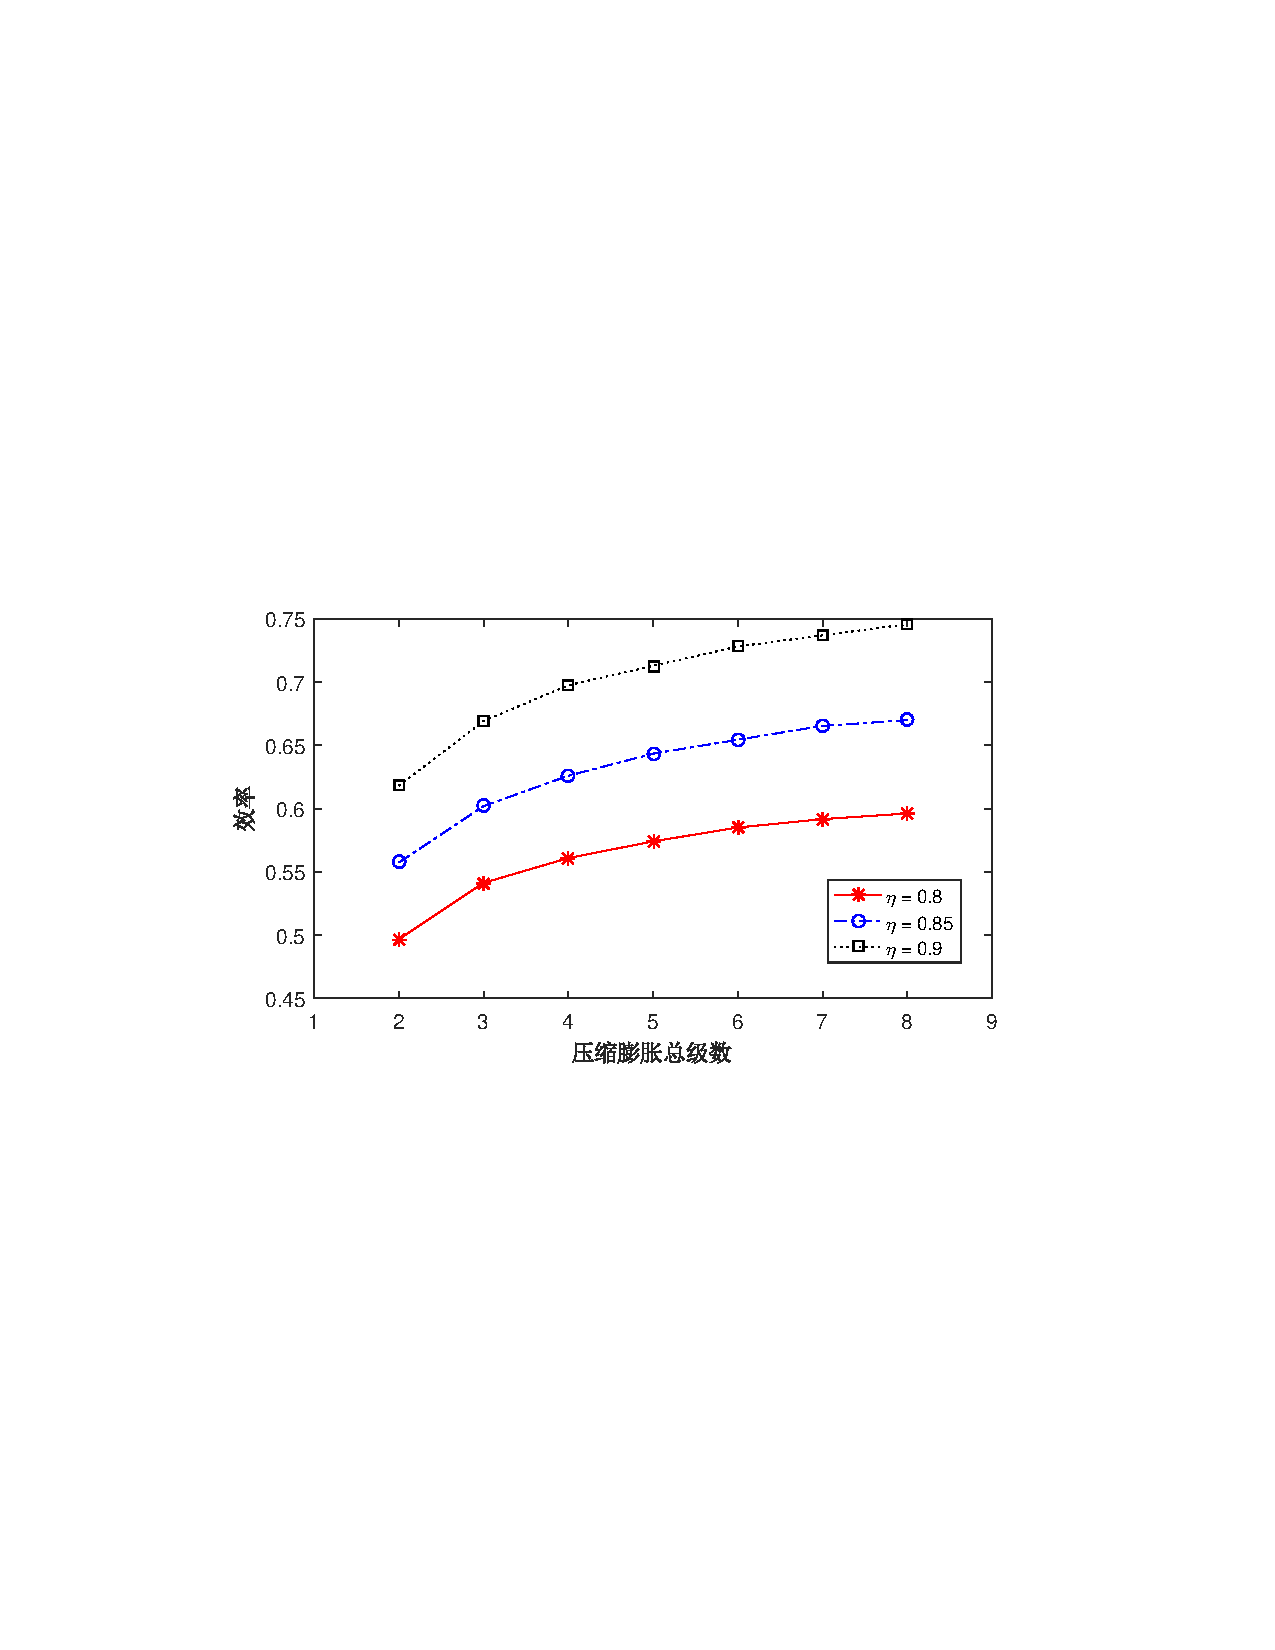
\includegraphics[scale=0.70]{figures/Chap1-6-Eff-Stage-No.pdf}
%  \caption{结构配置对电–电转换效率影响示意图}
%  \label{fig:Eff-Stage-No}
%\end{figure}

%在组件结构配置及参数优化方面,文献~\inlinecite{AA-CAES-Eff-Struc-13} 开展了压缩膨胀级数配置研究,通过仿真比较多种AA-CAES系统模型的功效率和㶲损失,给出了压缩机与透平膨胀机级数的最优组合。文献~\inlinecite{Ene-Exe-ACAES-17} 开展了AA-CAES系统的能量分析与㶲分析,指出最大㶲损出现在压缩机和透平,所设计的AA-CAES 系统电– 电转换效率达50\%,并指出通过增加压缩、膨胀级数和换热器可进一步减小㶲损,提高电–电转换效率。文献~\inlinecite{Thesis-Zhangxinjin} 系统分析了压缩膨胀级数组合对D-CAES及AA-CAES功效率及㶲效率的影响机制。文献~\inlinecite{Eff-Pow-MotCom-11} 关注系统运行过程中温度、压比及流量等参数对AA-CAES 效率的影响。但需说明的是,上述研究主要基于仿真方法配置AA-CAES结构,缺乏成熟优化方法指导设计,同时也很少考虑AA-CAES电站宽工况运行时工作点偏离设计点对结构配置及参数优化的影响机理。此外,在给定结构配置下温度及压比分配策略,以及宽工况运行条件下最优压缩发电运行的实现方式方面的探讨尚不充分。

%\subsubsection{宽工况运行效率}
%尽管通过组件结构及参数配置可在一定程度上确保AA-CAES在额定运行工况下达到较高的效率,但电力系统和综合能源系统对AA-CAES提出的宽工况运行要求\cite{EH-Form-14,IES-Disp-17} 将使其内部各组件频繁运行于非额定工况点,进而影响其电–电转换效率及综合能源利用效率。特别是在AA-CAES电站参与辅助服务时该问题将更加突出,在实际中需结合AA-CAES在一个周期内的整体运行工况分析其宽工况运行效率。

%具体而言,作为空气压力势能和压缩热能的解耦生产单元和耦合释能单元,压缩机和膨胀机(空气透平)在部分负载工况(非额定压缩和发电负荷)运行时效率变化明显。例如,压缩机、透平机械在额定设计点运行效率一般可达87\%-90\%,而50\%压缩/发电负荷时效率降至65\%-70\%,30\%压缩/发电负荷时效率甚至不及50\%~\cite{Eff-Pow-MotCom-11,CAES-Discharge-16}。 同时,作为空气压缩热能传输收集和传输释放单元的换热器亦存在部分负载运行特性,其换热系数易受热流流速(相应于压缩/发电负荷率)影响较大~\cite{HeatExch-Char-84,HE-Eff-CN-17}。

%文献~\inlinecite{CAES-PH-Char-11}分析了透平、膨胀机等组件运行特性对CAES系统效率的影响。文献~\inlinecite{ACAES-Conf-12} 建立了AA-CAES热力学模型,分析了温度、压比、工质流率等参数对其电-电转换效率的灵敏度。文献~\inlinecite{A-CAES-Therm-12,CAES-TES-Thermo-08} 分析了多级AA-CAES的热力学特性,强调了优化换热器的重要性。进一步,文献~\inlinecite{TES-Eff-CAES-13} 分析了蓄热系统对AA-CAES热力学特性的影响机制,定量评估了温度和压力对压缩热利用的影响效果。文献~\inlinecite{A-CAES-Dynamic-17} 计及内部压缩机与透平等组件的部分负载运行特性,建立了从组件性能到AA-CAES系统整体效率评估的仿真方法。

%综上,上述文献重点从热力学角度分析额定工况下AA-CAES系统运行参数对电-电转换效率或综合能效等的影响,较少探讨宽工况运行时AA-CAES系统的热力学特性及组件功-能转换机理,同时也较少关注非额定运行工况下压缩热能产生率、压缩热能损耗率、换热器传热特性及蓄热系统对储气库单位工质做功能力的提升机制等实际运行问题。本章第
%\ref{sec:part-load-energy}节与第\ref{sec:chap2-part-load-exergy}节将详细分析内部组件的部分负载特性与动态特性,进而分析AA-CAES系统级的宽工况运行特性,为揭示AA-CAES系统单位压缩功率压缩热能与压力势能产生量、单位发电功率压缩热能与压力势能消耗量、压缩与发电环节不同配比压缩热能与压力势能对压缩机耗功及透平出力的影响机理、压缩发电环节单位工质换热量与压缩发电功率水平的定量关系等奠定基础。

\section{基于热平衡的宽工况热力学仿真模型}
\label{sec:part-load-energy}
AA-CAES在削峰填谷、旋转备用、无功支撑、多能联供等典型场景的应用,要求其具有宽工况运行能力(20\%-110\%压缩功率/膨胀功率运行)。在宽工况运行条件下,压缩机、膨胀机等能量转换组件的运行特性(如效率等)变化明显。同时,换热器等能量转移组件的传热系数受到热工质流率的影响,不同质量流率下传热系数变化明显
\cite{HeatExch-Char-84,HE-Eff-CN-17},影响压缩热能的收集和回馈,进而改变AA-CAES系统的电-电转换性能与热电联供性能。文献\inlinecite{A-CAES-Dynamic-17}针对采用高温储热技术收集空气压缩热能的典型两级压缩两级膨胀系统的分析表明,当储热效率\footnote{此处的储热效率仅针对填充床储热型AA-CAES,不能适用于双罐储热型AA-CAES,其定义为一个循环周期内流出与流入填充床储热系统的空气焓值之比。}达到90\% 以上时,额定工况运行时AA-CAES 电-电效率可达74\%,当宽工况运行时,其效率降为64\%。因此,当前采用的根植于电池储能的固定效率模型难以计及压缩机、膨胀机、换热器等组件的部分负载运行特性对AA-CAES 整体性能的影响。本节基于热力学第一定律建立能量转换组件与能量转移组件的部分负载热力学模型,以及能量存储组件的热力学动态模型,最后给出AA-CAES系统级的宽工况热力学仿真模型。

\subsection{能量转换类模块}

对AA-CAES各应用形式而言,一般均包含压缩机、空气透平等能量转换类组件,本小节分别给出二者在额定工况以及部分负载工况下的稳态热力学模型。

\subsubsection{压缩机}
\label{sec:part-load-energy-compressor}
%\subsubsection{部分负载特性概述}

\textbf{(1)额定工况能量平衡关系}

%第$i$级压缩机等熵压缩出口温度满足,
%\begin{equation}
%\label{equ:comp-iso-temp}
%T_{c,i}^{out,is} = T_{c,i}^{in}{\left( {{\beta _{c,i}}} \right)^{\frac{{k - 1}}{k}}}
%\end{equation}
%其中,$T_{c,i}^{in}$ 为压缩机入口空气温度,$k$ 为空气绝热指数,取值为1.4。

第$i$级压缩机出口空气温度可由等熵效率计算\cite{Eng-Thermo-83},即
% \begin{equation}
%\label{equ:comp-real-temp-1}
%{\eta _{c,i}} = \frac{{T_{c,i}^{out,is} - T_{c,i}^{in}}}{{T_{c,i}^{out} - T_{c,i}^{in}}}
%\end{equation}
%即,第$i$级压缩机实际出口空气温度为
 \begin{equation}
\label{equ:comp-real-temp-2}
T_{c,i}^{out} = \frac{1}{{{\eta _{c,i}}}}T_{c,i}^{in}({{{({{\beta _{c,i}}})}^{\frac{{k - 1}}{k}}} + {\eta _{c,i}} - 1})
\end{equation}
其中,$\eta _{c,i}$ 为压缩机等熵效率;$T_{c,i}^{in}$ 为压缩机入口空气温度;$k$ 为空气绝热指数,取值为1.4\footnote{更精确的计算可采用多变指数代替绝热指数$k$, 本文不予考虑。};${\beta _{c,i}}$ 为压缩机压比。

第$i$级压缩机实际耗功及所有压缩机总耗功分别为,
\begin{subequations}
\begin{gather}
{W_{c,i}} = {\dot m_c}c_p^a({T_{c,i}^{out} - T_{c,i}^{in}})\label{equ:comp-power}\\
{W_c} = \sum\limits_{i = 1}^{{N_c}} {} {W_{c,i}} \label{equ:comp-power-total}
\end{gather}
\end{subequations}
其中, $\dot m_c$为压缩机空气质量流率;$N_c$ 为压缩机级数;$c_p^a$ 为空气的定压比热容\footnote{若需进行更精确的仿真,可采用焓值计算耗功
\cite{Eng-Thermo-83},即${W_{c,i}} = {\dot m_c}({h_{c,i}^{out} - h_{c,i}^{in}})$。}。

第$i$级压缩机出口空气压力为,
\begin{equation}
\label{equ:comp-pressure}
p_{c,i}^{out} = p_{c,i}^{in}{\beta _{c,i}}
\end{equation}
其中,$p_{c,i}^{in}$ 为进口空气压力; $p_{c,i}^{out}$为出口空气压力。

后文研究中不计及压缩机的部分负载运行特性时,即可采用额定工况稳态热力学模型(\ref{equ:comp-real-temp-2})-(\ref{equ:comp-pressure})。

\textbf{(2)部分负载特性解析模型}

作为空气压力势能和压缩热能的解耦生产单元,压缩机的压比$\beta _{c,i}$与等熵效率$\eta _{c,i}$ 随其运行工况变化。在额定设计点,压缩机的等熵效率一般可达87\%-90\%,而50\% 压缩负载时其等熵效率降至65\%-70\%,30\%压缩负载时等熵效率甚至不及50\% ~\cite{CAES-Review-18-Rui-operation}。文献
\inlinecite{A-CAES-Therm-12}指出采用变效率方程(二次曲线)来刻画压缩机的部分负载运行特性,即
\begin{equation}
\label{equ:comp-eff-quad}
{\eta _{c,i}} = {({{\eta _{c,i}}})_0} - {\alpha _c}{({{{({{\beta _{c,i}}})}_0} - {\beta _{c,i}}})^2}
\end{equation}
其中,${\alpha _c}$ 为常数;${(\cdot)_0}$ 表示设计工况下的参数,后文相同。但该方法仅能给出等熵效率随压比变化的近似关系,难以揭示压缩机部分负载运行时非额定质量流率引起压比及等熵效率变化的物理本质。文献\inlinecite{Compressor-thermo-02}给出了部分负载运行工况下单轴燃气轮机中压缩机及透平的特性曲线的解析表达式,为仿真压缩机的部分负载运行特性提供了依据。文献\inlinecite{Compressor-Review-17}给出了压缩机特性参数的典型回归方法,可用于燃气轮机热力学仿真模型的构建。鉴于文献\inlinecite{Compressor-thermo-02}中的部分负载解析方法在填充床储热型AA-CAES的热力学特性分析\cite{A-CAES-Dynamic-17}、 低温储热型AA-CAES的㶲特性分析~\cite{CHS-CAES-off-19}、AA-CAES 型CCHP系统\cite{AA-CAES-Simulation-19}及其它诸多热力系统仿真中得到较多应用,本节引入文献\inlinecite{Compressor-thermo-02} 中的压缩机特性图的解析表达式来描述其部分负载特性。

部分负载运行时压缩机的实际压比及实际等熵效率可分别表示为\cite{Compressor-thermo-02,A-CAES-Dynamic-17},
\begin{subequations}
\label{eq:com-iso-eff-off}
\begin{gather}
\frac{{{\beta _{c,i}}}}{{{{({{\beta _{c,i}}})}_0}}} = {a_{1,i}}{({{{\dot G}_{c,i}}})^2} + {a_{2,i}}{\dot G_{c,i}} + {a_{3,i}}\label{equ:comp-press-part}\\
\frac{{{\eta _{c,i}}}}{{{{({{\eta _{c,i}}})}_0}}} = [{1 - c{{({1 - {{\dot n}_{c,i}}})}^2}}]({{{\dot n}_{c,i}}/{{\dot G}_{c,i}}})({2 -({{{\dot n}_{c,i}}/{{\dot G}_{c,i}}})})\label{equ:comp-eff-part}
\end{gather}
\end{subequations}
其中,($a_{1,i}$, $a_{2,i}$, $a_{3,i}$)为表征转速对压比影响的因子;${\dot G_{c,i}}$ 与 ${\dot n_{c,i}}$ 分别为无量纲降阶流率与降阶转速,满足
\begin{subequations}
\label{eq:com-mass-off}
\begin{gather}
{\dot G_{c,i}} = [{{{\dot m}_c}\frac{{{{({T_{c,i}^{in}})}^{0.5}}}}{{p_{c,i}^{in}}}}]/{[{{{\dot m}_c}\frac{{{{({T_{c,i}^{in}})}^{0.5}}}}{{p_{c,i}^{in}}}}]_0}\label{equ:reduced-comp-mass-flow}\\
{\dot n_{c,i}} = [{{n_c}{{({T_{c,i}^{in}})}^{-0.5}}}]/{[{{n_c}{{({T_{c,i}^{in}})}^{-0.5}}}]_0}\label{equ:reduced-comp-speed}
\end{gather}
\end{subequations}
其中,$n_c$为压缩机转速,对于采用变频调速等方式调节各级压缩机转速的实际系统,可修正(\ref{equ:reduced-comp-speed})中的$n_c$为$n_{c,i}$。定义中间变量,
\begin{equation}
\label{equ:comp-mid-var-1}
{a_{0,i}} = [{{b_1}({1 - \frac{{{b_2}}}{{{{\dot n}_{c,i}}}}}) + {{\dot n}_{c,i}}{{({{{\dot n}_{c,i}} - {b_2}})}^2}}]
\end{equation}
则其它时变系数参数满足:
\begin{equation}
\label{equ:comp-mid-var-2}
{a_{1,i}} = \frac{{{{\dot n}_{c,i}}}}{{{a_{0,i}}}}, {a_{2,i}} = \frac{{({{b_1} - 2{b_2}\dot n_{c,i}^2})}}{{{a_{0,i}}}}, {a_{3,i}} = \frac{{{b_2}^2\dot n_{c,i}^3 - {b_1}{b_2}{{\dot n}_{c,i}}}}{{{a_{0,i}}}}
\end{equation}
其中,($b_1$, $b_2$, $c$) 为常系数,其典型取值为(1.8, 1.4, 0.3)~\cite{Compressor-thermo-02}, (0.36, 1.06, 0.3)~\cite{A-CAES-Dynamic-17}, (1.8, 0.93,0.3)~\cite{AA-CAES-Simulation-19}或(1.7, 0.93, 0.4)~\cite{AA-CAES-Simulation-19},对实际给定的压缩机可由其特性图进行拟合
\cite{Compressor-Off-Design-05},但需满足$b_1^{1/3}\le 2b_2/3$。

基于部分负载解析模型(\ref{eq:com-iso-eff-off})-(\ref{equ:comp-mid-var-2})可得如图~\ref{fig:Comp-Ratio-off-design}~ 及图~\ref{fig:Eff-part-load}~所示的压缩机压比及等熵效率的典型曲线。如此,基于部分负载工况下的实际压比及实际等熵效率,在给定实际入口温度及实际入口压力的条件下即可获得第$i$ 级压缩机的实际耗功、实际出口温度、实际出口压力。

\begin{figure}[H] % use float package if you want it here
  \centering
  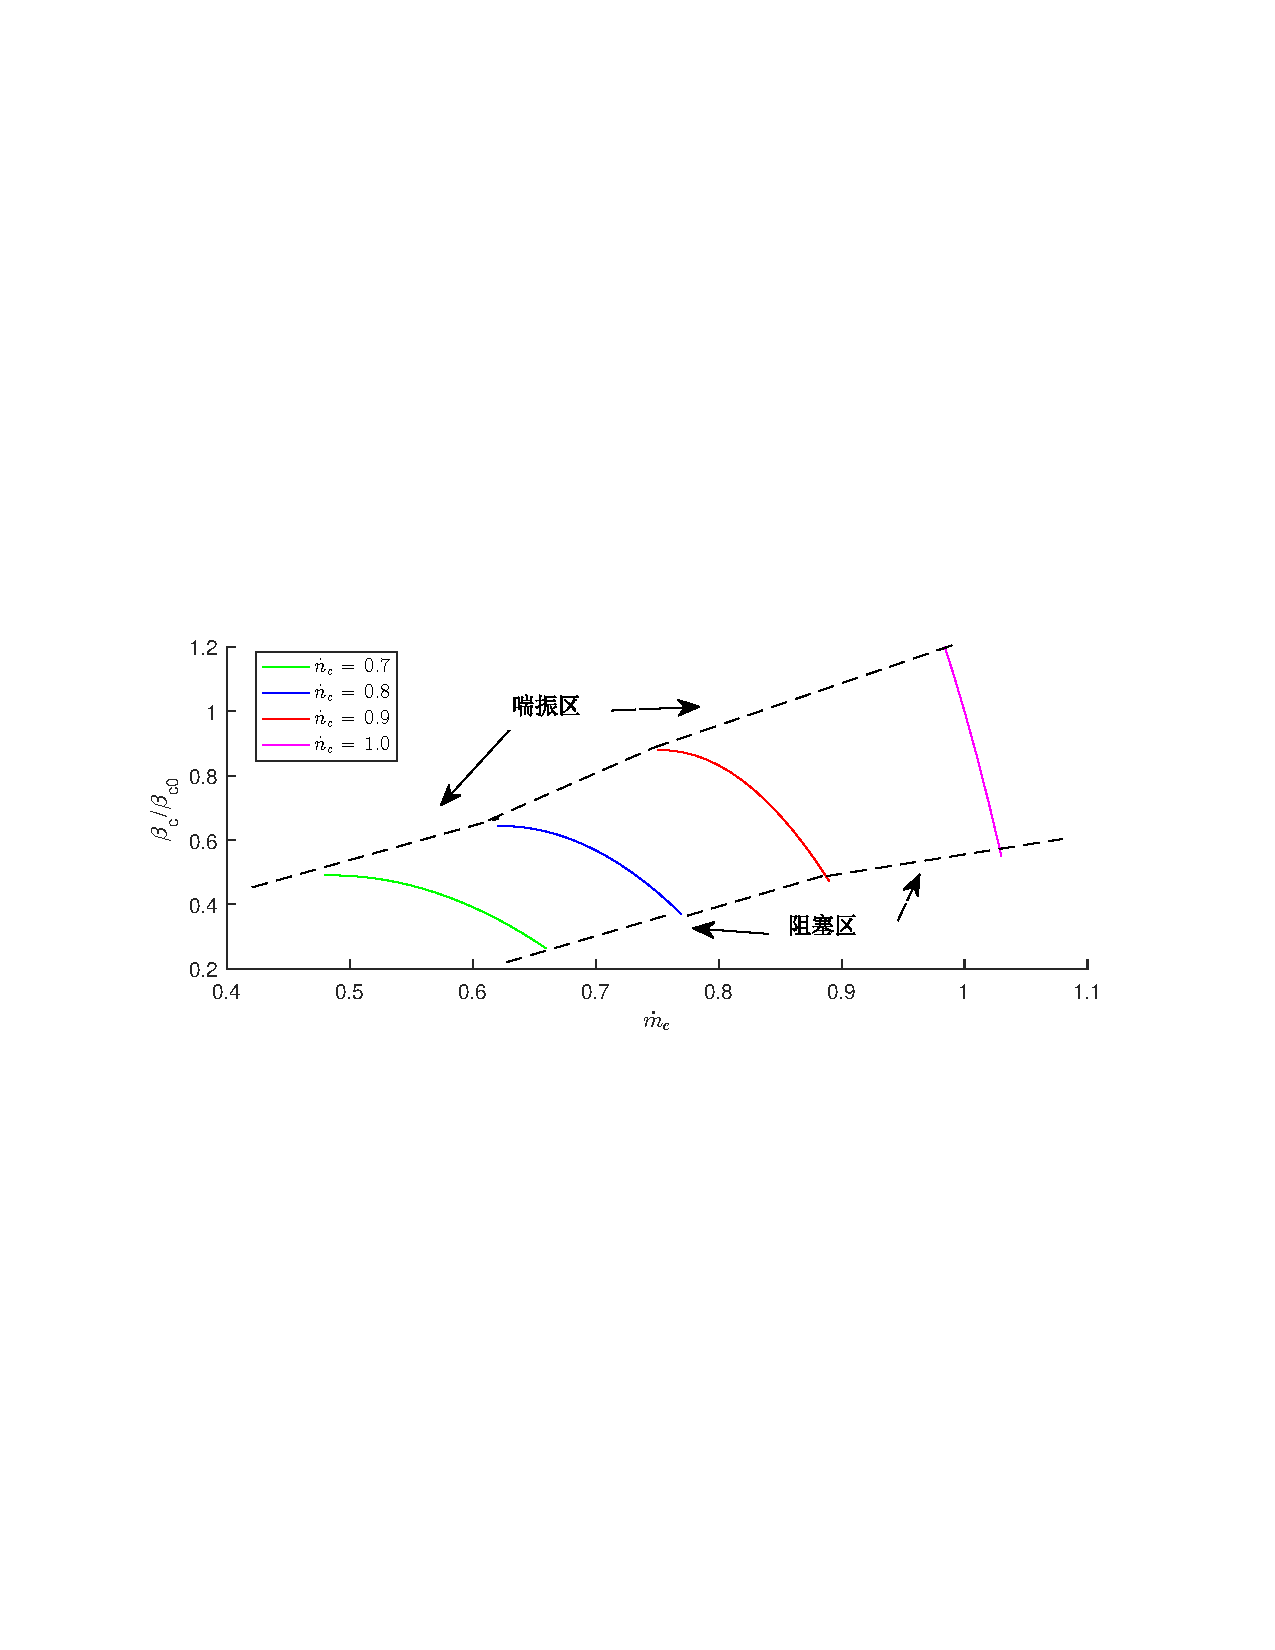
\includegraphics[scale=0.70]{figures/Chap2-2-Comp-Ratio-off-design.pdf}
  \caption{基于解析模型的压缩机部分负载压比}
  \label{fig:Comp-Ratio-off-design}
\end{figure}

\begin{figure}[H] % use float package if you want it here
  \centering
  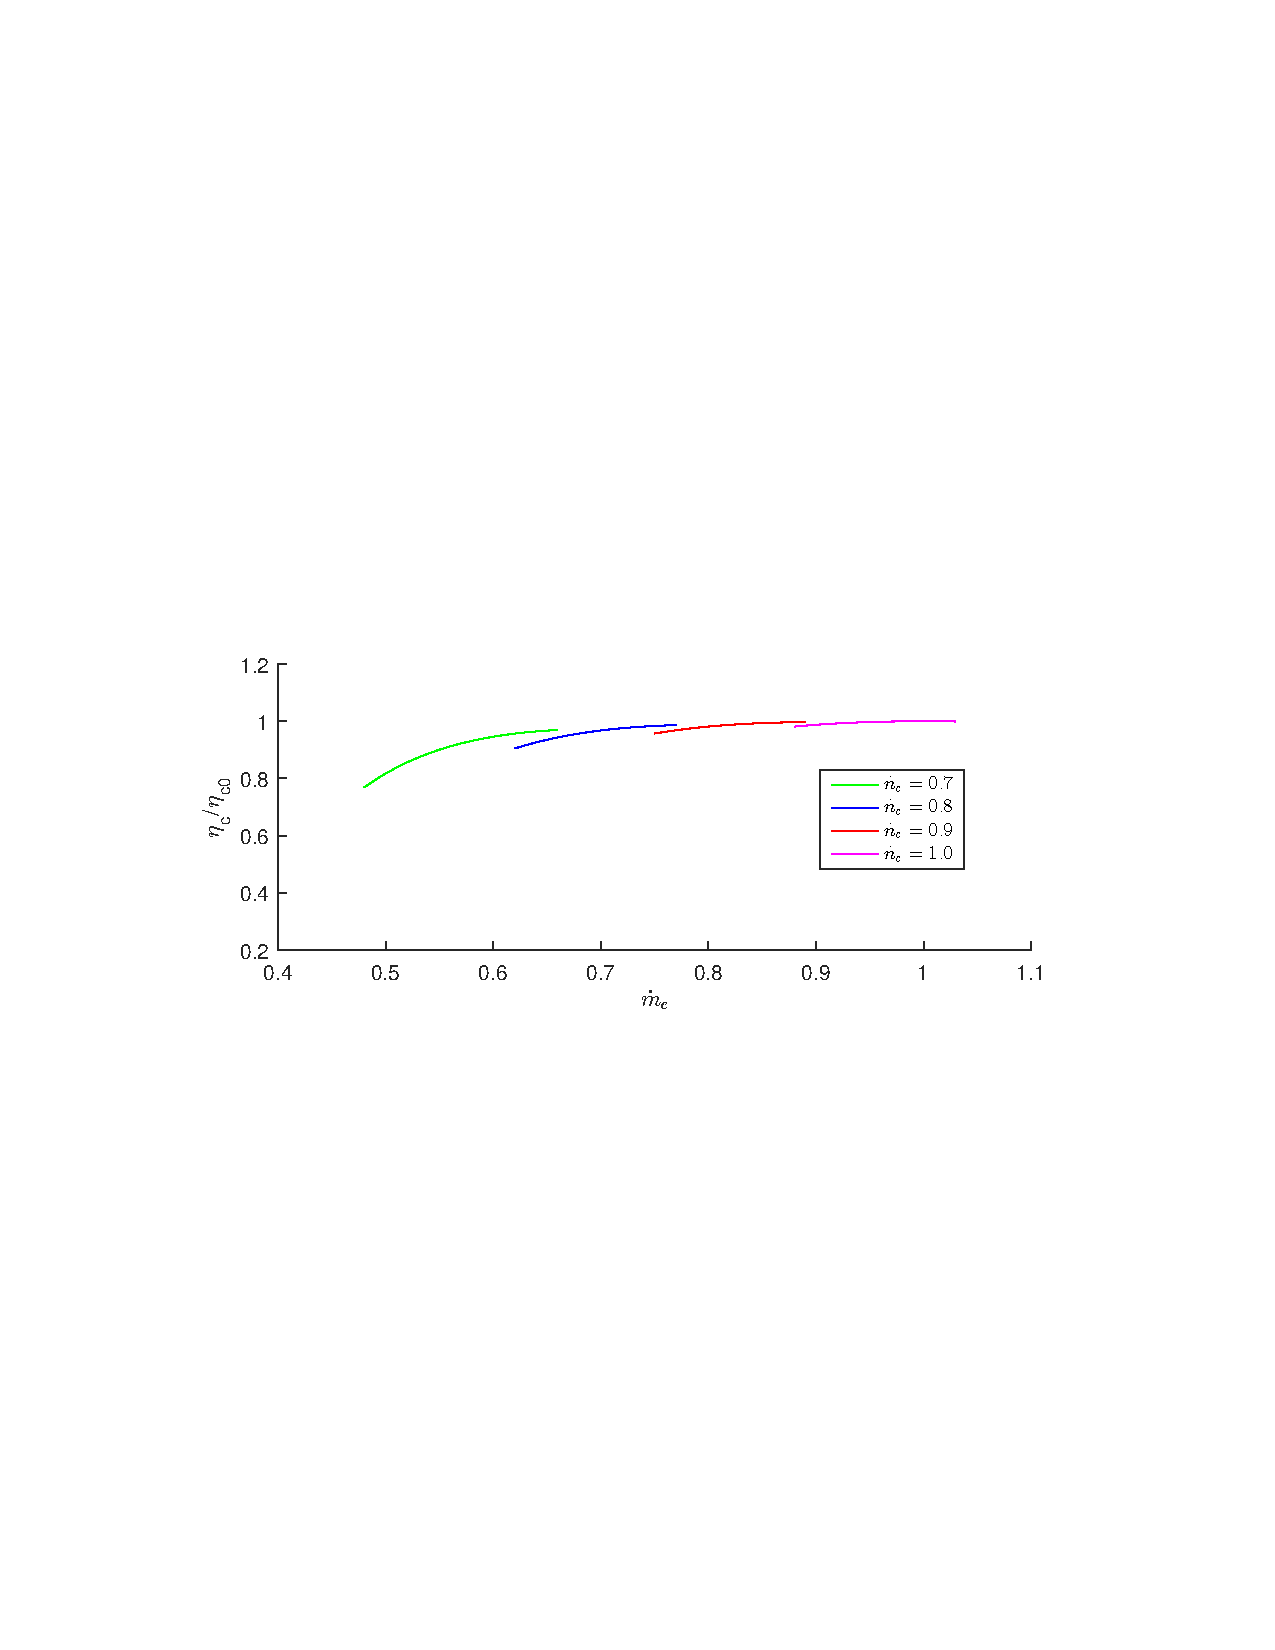
\includegraphics[scale=0.80]{figures/Chap2-3-Eff-part-load.pdf}
  \caption{基于解析模型的压缩机部分负载等熵效率}
  \label{fig:Eff-part-load}
\end{figure}

压缩机额定工况热力学模型(\ref{equ:comp-real-temp-2})-(\ref{equ:comp-pressure})及部分负载热力学模型(\ref{equ:comp-real-temp-2})-(\ref{equ:comp-mid-var-2}) 中的变量如表~\ref{tab:comp-thermo-para}~所示。在实际运行中的任一给定时刻,第1级压缩机入口温度$T_{c,1}^{in}$及入口压力$p_{c,1}^{in}$ 为确定值,外界电网调度指令会给出实时功率$W_c$,其它边界条件可通过后续组件确定。

\begin{table}[htb]
  \centering
  \begin{minipage}[t]{0.9\linewidth} % 如果想在表格中使用脚注,minipage是个不错的办法
  \caption{压缩机部分负载热力学模型变量表}
  \label{tab:comp-thermo-para}
    \begin{tabularx}{\linewidth}{cccccc}
      \toprule[1.5pt]
      {\heiti 变量} & {\heiti 物理意义} & {\heiti 单位} &  {\heiti 变量} & {\heiti 物理意义} & {\heiti 单位} \\\midrule[1pt]
      ${W_{c,i}}$ & 耗(电)功 & kW  &  ${\dot m_c}$ & 空气质量流率 & kg/s \\
      ${\beta _{c,i}}$ & 实际压比 & —— &  ${\eta _{c,i}}$ & 等熵效率 & —— \\
      $p_{c,i}^{in}$ & 空气进口压力 & kPa & $p_{c,i}^{out}$ & 空气出口压力 & kPa \\
      $T_{c,i}^{in}$ & 空气进口温度 & K & $T_{c,i}^{out}$ & 空气出口温度 & K \\
      ${n_{c,i}}$ & 实际转速 & r/min & $\dot n_{c,i}$ & 无量纲降阶转速 & —— \\
      $a_{0,i}$, $a_{1,i}$ & 中间变量 & —— & $a_{2,i}$, $a_{3,i}$ & 中间变量 & ——\\
      ${\dot G_{c,i}}$ &  无量纲降阶质量流率 &  —— & & &\\
      \bottomrule[1.5pt]
    \end{tabularx}
  \end{minipage}
\end{table}

\subsubsection{空气透平}
\label{sec:part-load-energy-turbine}


\textbf{(1)额定工况能量平衡关系}

%第$i$级膨胀机等熵膨胀出口温度满足,
%\begin{equation}
%\label{equ:turb-iso-temp}
%T_{e,i}^{out,is} = T_{e,i}^{in}/{\left( {{\beta _{e,i}}} \right)^{\frac{{k - 1}}{k}}}
%\end{equation}

第$i$级膨胀机出口空气温度可由等熵效率计算\cite{Eng-Thermo-83},
% \begin{equation}
%\label{equ:turb-real-temp-1}
%{\eta _{c,i}} = \frac{{T_{c,i}^{out,is} - T_{c,i}^{in}}}{{T_{c,i}^{out} - T_{c,i}^{in}}}
%\end{equation}
%
%第$i$级膨胀机实际出口温度为,
 \begin{equation}
\label{equ:turb-real-temp-2}
T_{e,i}^{out} = T_{e,i}^{in}({1 - {\eta _{e,i}} + {\eta _{e,i}}{{({{\beta _{e,i}}})}^{\frac{{1 - k}}{k}}}})
\end{equation}
其中,$\eta _{e,i}$为透平等熵效率;$T_{e,i}^{in}$ 为透平入口空气温度;$\beta _{e,i}$ 为透平膨胀比。

第$i$级膨胀机实际做功及所有膨胀机做的总功为,
\begin{subequations}
\label{equ:turb-power-all}
\begin{gather}
{W_{e,i}} = {\dot m_e}c_p^a({T_{e,i}^{in} - T_{e,i}^{out}})\label{equ:turb-power}\\
{W_e} = \sum\limits_{i = 1}^{{N_e}} {{W_{e,i}}}\label{equ:turb-power-total}
\end{gather}
\end{subequations}
其中,$\dot m_e$为膨胀机空气质量流率;$N_e$ 为透平级数。

第$i$级膨胀机实际出口空气压力为,
\begin{equation}
\label{equ:turb-pressure}
p_{e,i}^{out} = p_{e,i}^{in}/{\beta _{e,i}}
\end{equation}
其中,$p_{e,i}^{in}$ 为进口空气压力;$p_{e,i}^{out}$为出口空气压力。

与压缩机类似,后文研究中不计及空气透平的部分负载特性时,即可采用额定工况稳态热力学模型(\ref{equ:turb-real-temp-2})-(\ref{equ:turb-pressure})。

\textbf{(2)部分负载特性解析模型}

空气透平也存在类似于压缩机的部分负载运行特性,其等熵效率会随着运行工况发生大幅变化。在额定工况下透平的等熵效率可达85\%-90\%,而在50\%负载工况下等熵效率降至65\%-75\%\cite{CAES-Review-18-Rui-operation,CAES-Discharge-16}。 在膨胀释能过程中,随着储气压力的降低,储气室出口空气温度和压力均会变化~\footnote{一般认为,存在出口侧节流阀时仅入口温度会变化,不存在节流阀时入口温度与入口压力均会变化。},从而引起透平的部分负载工况运行。为刻画等熵效率随部分负载运行工况(通常由质量流率及转速偏离额定工况引起)的变化特性,引入膨胀机的部分负载特性解析表达式。实际部分负载运行时等熵效率特性满足\cite{Compressor-thermo-02, AA-CAES-Simulation-19},
\begin{equation}
\label{equ:turb-eff-part}
{\eta _{e,i}}/{({{\eta _{e,i}}})_0} = [{1 - {b_0}{{({1 - {{\dot n}_{e,i}}})}^2}}]({{{\dot n}_{e,i}}/{{\dot G}_{e,i}}})({2 -({{{\dot n}_{e,i}}/{{\dot G}_{e,i}}})})
\end{equation}
其中,$b_0$为常数,典型取值为0.3\cite{Compressor-thermo-02}。

由改进弗留格尔公式可知,无量纲节省(降阶)质量流率与降阶转速满足\cite{Compressor-thermo-02, AA-CAES-Simulation-19},
\begin{subequations}
\begin{gather}
{\dot G_{e,i}} = [{{{\dot m}_e}\frac{{{{({T_{e,i}^{in}})}^{0.5}}}}{{p_{e,i}^{in}}}}]/{[{{{\dot m}_e}\frac{{{{( {T_{e,i}^{in}})}^{0.5}}}}{{p_{e,i}^{in}}}}]_0} \label{equ:reduced-turb-mass-flow} \\
{\dot n_{e,i}} = [{{n_{e,i}}{{({T_{e,i}^{in}})}^{ - 0.5}}}]/{[{{n_{e,i}}{{({T_{e,i}^{in}})}^{ - 0.5}}} ]_0}\label{equ:reduced-turb-speed}
\end{gather}
\end{subequations}
透平实际膨胀比满足\cite{AA-CAES-Simulation-19},
\begin{equation}
\label{equ:turb-pressure-part}
\frac{{{{\dot m}_e}}}{{{{({{{\dot m}_e}})}_0}}} = {\alpha _i}\sqrt {\frac{{{{({T_{e,i}^{in}})}_0}}}{{T_{e,i}^{in}}}} \sqrt {\frac{{\beta _{e,i}^2 - 1}}{{{{({\beta _{e,i}^2})}_0} - 1}}}
\end{equation}
其中,$\alpha_i$为表征转速变化对膨胀比影响的因子,满足$\alpha_i=\sqrt{1.4-0.4n_{e,i}/(n_{e,i})_0}$。

基于部分负载解析模型(\ref{equ:turb-eff-part})-(\ref{equ:turb-pressure-part}),可得如图\ref{fig:Turb-Ratio-off-design}及图\ref{fig:Turb-Eff-part-load}所示的空气透平膨胀比及等熵效率典型曲线。

\begin{figure}[H] % use float package if you want it here
  \centering
  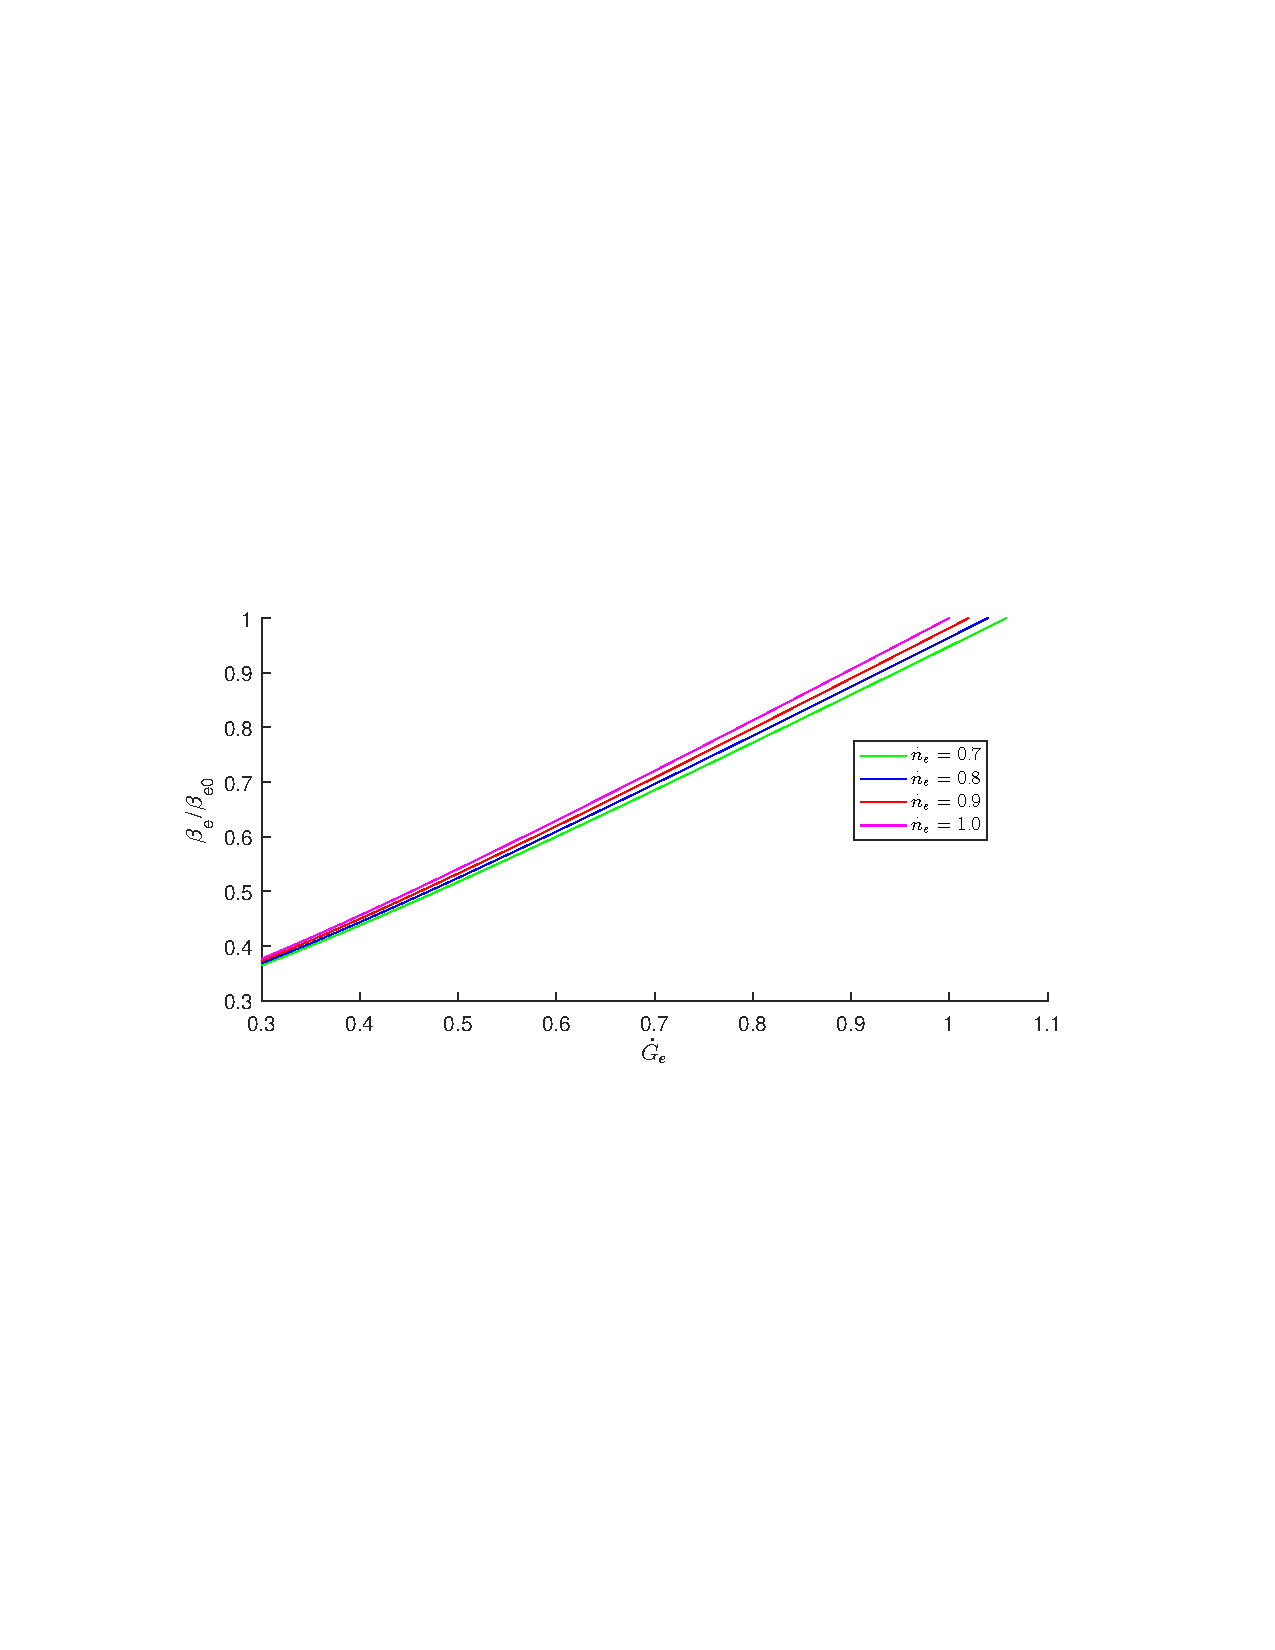
\includegraphics[scale=0.65]{figures/Chap2-2-Turb-Ratio-off-design.pdf}
  \caption{基于解析模型的空气透平部分负载膨胀比}
  \label{fig:Turb-Ratio-off-design}
\end{figure}

\begin{figure}[H] % use float package if you want it here
  \centering
  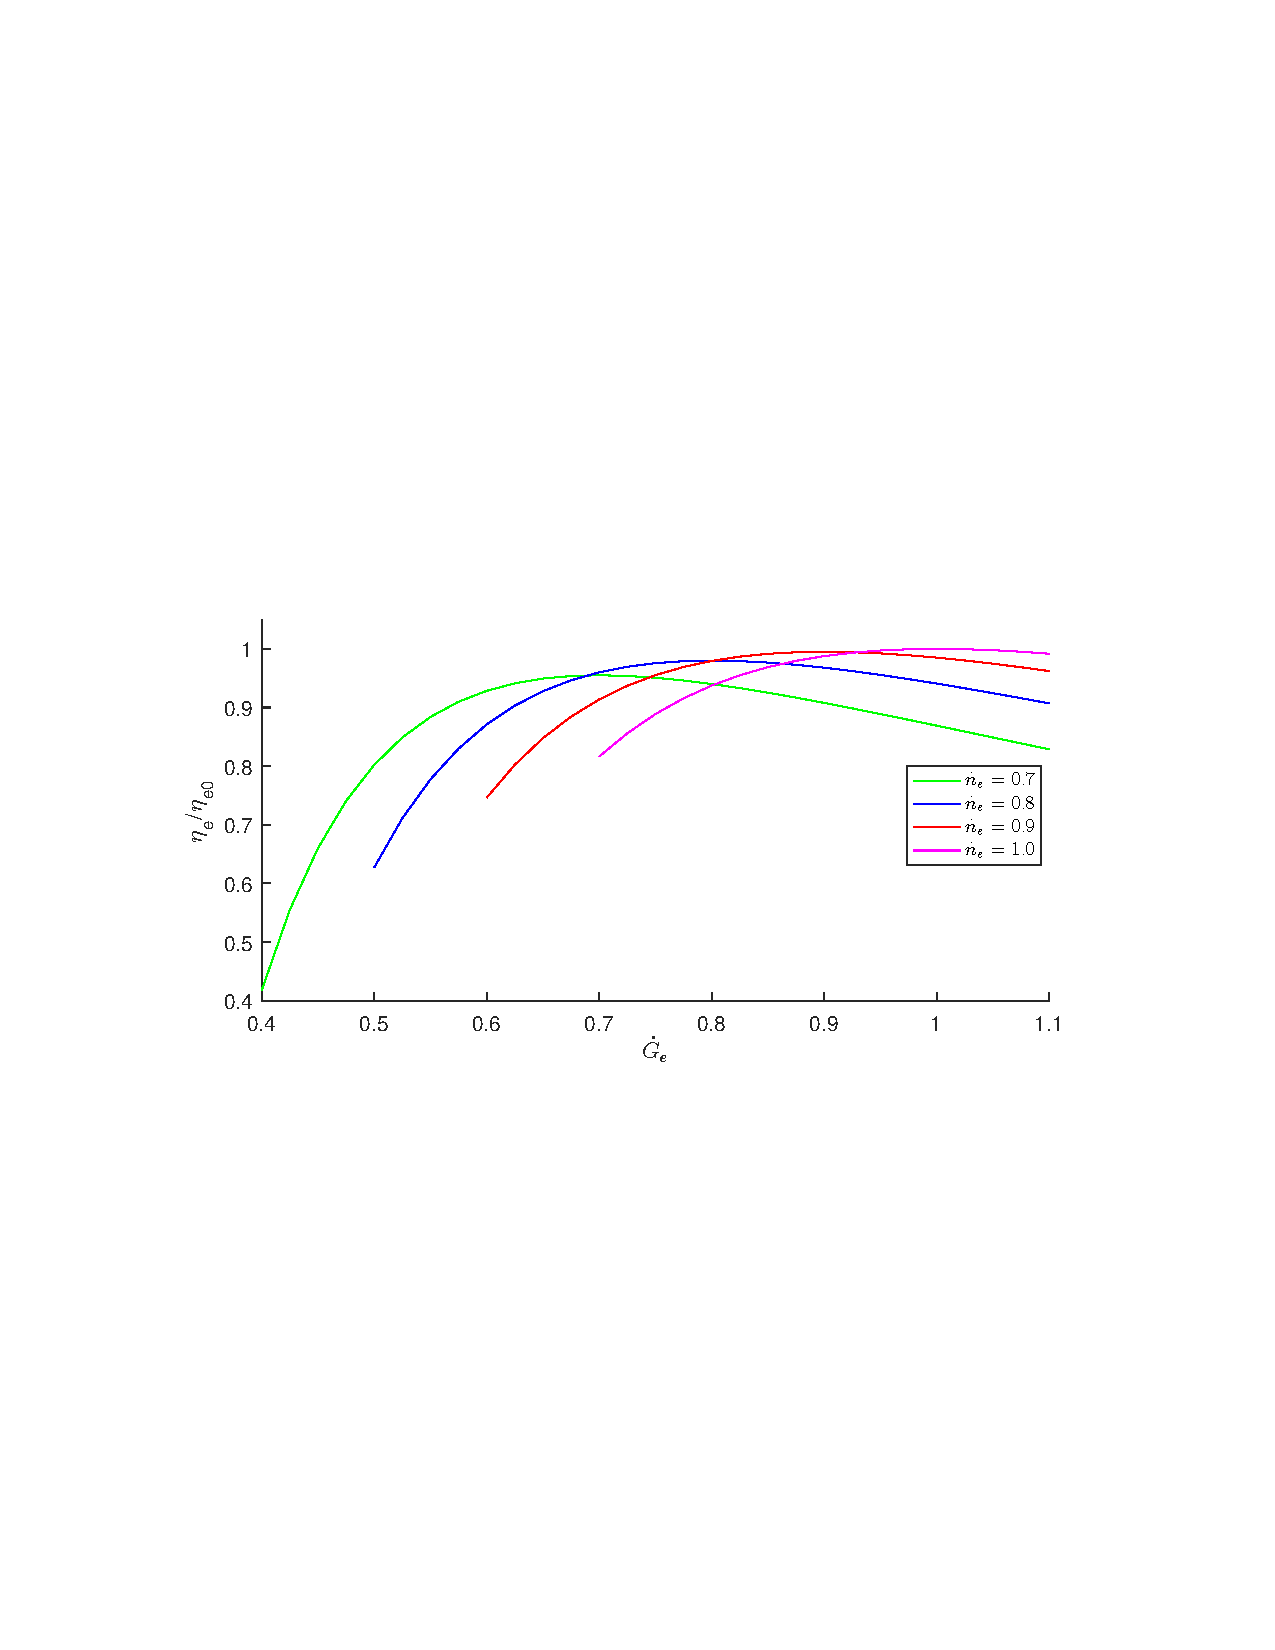
\includegraphics[scale=0.65]{figures/Chap2-3-Turb-Eff-part-load.pdf}
  \caption{基于解析模型的空气透平部分负载等熵效率}
  \label{fig:Turb-Eff-part-load}
\end{figure}

综上,透平的额定工况热力学模型(\ref{equ:turb-real-temp-2})-(\ref{equ:turb-pressure})及部分负载热力学模型(\ref{equ:turb-real-temp-2})-(\ref{equ:turb-pressure-part}) 中的变量如表~\ref{tab:turb-thermo-para}~所示。在实际运行中的任一给定时刻,外界电网调度指令会给出实时功率需求$W_e$,其它边界条件可通过后续组件确定。

\begin{table}[htb]
  \centering
  \begin{minipage}[t]{0.9\linewidth} % 如果想在表格中使用脚注,minipage是个不错的办法
  \caption{空气透平部分负载热力学模型变量表}
  \label{tab:turb-thermo-para}
    \begin{tabularx}{\linewidth}{cccccc}
      \toprule[1.5pt]
      {\heiti 变量} & {\heiti 物理意义} & {\heiti 单位} &  {\heiti 变量} & {\heiti 物理意义} & {\heiti 单位} \\\midrule[1pt]
      ${W_{e,i}}$ & 做功(电) & kW  &  ${\dot m_e}$ & 空气质量流率 & kg/s \\
      ${\beta _{e,i}}$ & 实际膨胀比 & —— &  ${\eta _{e,i}}$ & 等熵效率 & —— \\
      $p_{e,i}^{in}$ & 空气进口压力 & kPa & $p_{e,i}^{out}$ & 空气出口压力 & kPa \\
      $T_{e,i}^{in}$ & 空气进口温度 & K & $T_{e,i}^{out}$ & 空气出口温度 & K \\
      ${n_{e,i}}$ & 实际转速 & r/min & $\dot n_{e,i}$ & 无量纲降阶转速 & —— \\
      ${\dot G_{e,i}}$ &  无量纲降阶质量流率 &  —— & & & \\
      \bottomrule[1.5pt]
    \end{tabularx}
  \end{minipage}
\end{table}

\subsection{能量转移类模块}
\label{sec:part-load-energy-he}

对AA-CAES各应用形式而言,一般均含有压缩侧换热器与膨胀侧换热器等能量转移类模块,本小节分别给出二者在额定工况及部分负载工况下的稳态热力学模型。

\subsubsection{压缩侧换热器}
定义第$i$ 级换热器的空气侧入口温度为 $T_{c,HX,i}^{a,in}$ ,载热工质(Heat Transfer Fluid, HTF)的入口温度为$T_{c,HX,i}^{HTF,in}$,则换热器出口侧空气温度及HTF 温度分别为,
\begin{subequations}
\label{eq:he-comp-temp-out}
\begin{gather}
T_{c,HX,i}^{a,out} = T_{c,HX,i}^{a,in} + \Phi _{c,i}^{HX}/({c_p^a\dot m_c^a}) \label{equ:he-comp-temp-air-out} \\
T_{c,HX,i}^{HTF,out} = T_{c,HX,i}^{HTF,in} - \Phi _{c,i}^{HX}/({c_p^{HTF}\dot m_{c,i}^{HTF}}) \label{equ:he-comp-temp-HTF-out}\\
\Phi _{c,i}^{HX} = {\varepsilon _{c,i}}C_{c,i}^{\min }({T_{c,HX,i}^{HTF,in} - T_{c,HX,i}^{a,in}})\label{equ:he-comp-thermal}
\end{gather}
\end{subequations}
其中,$\dot m_{c,i}^{HTF}$ 为HTF质量流率;$c_p^{HTF}$为HTF 定压比热容;$\Phi _{c,i}^{HX}$ 为换热器的换热功率;$C_{c,i}^{\min}$为换热器最小热容;${\varepsilon _{c,i}}$ 为换热器效能,具体表达式视实际换热器类型而定,图\ref{fig:CAES-thermal-struc}中压缩侧采用的逆流换热器的效能${\varepsilon _{c,i}}$ 满足\cite{Heat-mass-transfer-11},
\begin{subequations}
\begin{gather}
{\varepsilon _{c,i}} = \frac{{1 - \exp [{ - NT{U_{c,i}}({1 - C_{c,i}^{HX}})}]}}{{1 - C_{c,i}^{HX}\exp [{ - NT{U_{c,i}}({1 - C_{c,i}^{HX}})}]}}\label{equ:he-comp-eff-1}
%{\varepsilon _{c,i}} = \frac{{1 - \exp \left[ { - NT{U_{c,i}}\left( {1 + C_{c,i}^{HX}} \right)} \right]}}{{1 + C_{c,i}^{HX}}}\label{equ:he-comp-eff-2}
\end{gather}
\end{subequations}
其中,$NT{U_{c,i}}$ 与$C_{c,i}^{HX}$分别为换热器的传热单元数与热容比,满足\cite{Heat-mass-transfer-11}
\begin{subequations}
\begin{gather}
NT{U_{c,i}} = U_{c,i}A_{c,i}/C_{c,i}^{\min }, C_{c,i}^{HX} = C_{c,i}^{\min }/C_{c,i}^{\max }\label{equ:he-comp-NTU-C}\\
C_{c,i}^{\min } = {({{{\dot m}_c}c_p^a,\dot m_{c,i}^{HTF}c_p^{HTF}})_{\min }}\label{equ:he-comp-Cmin}\\
C_{c,i}^{\max } = {({{{\dot m}_c}c_p^a,\dot m_{c,i}^{HTF}c_p^{HTF}})_{\max }}\label{equ:he-comp-Cmax}
\end{gather}
\end{subequations}
其中,$C_{c,i}^{\max }$为换热器最大热容;$U_{c,i}$与$A_{c,i}$分别为换热系数与换热面积,不考虑部分负载特性时,$U_{c,i}$可视为常数。

第$i$级换热器所需的HTF的质量流率满足,
\begin{equation}
\label{equ:he-comp-mass-flow}
\dot m_{c,i}^{HTF} = \frac{{{{\dot m}_c}c_p^a({T_{c,HX,i}^{a,in} - T_{c,HX,i}^{a,out}} )}}{{c_p^{HTF}( {T_{c,HX,i}^{HTF,out} - T_{c,HX,i}^{HTF,in}})}}
\end{equation}

考虑换热器的压损特性,则换热器出口的空气压力为,
\begin{subequations}
\begin{gather}
p_{c,HX,i}^{out} = \eta _{c,HX,i}^pp_{c,HX,i}^{in}\label{equ:he-comp-pressure-out}
\end{gather}
\end{subequations}
其中,$\eta _{c,HX,i}^p$为换热器压力的保持系数\cite{Thesis-Lixuemei},且满足$\eta _{c,HX,i}^p = 1 - \frac{{0.0083{\varepsilon _{c,i}}}}{{1 - {\varepsilon _{c,i}}}}$,系数0.0083可视实际换热器类型进行调整;若不考虑压损,设置$\eta _{c,HX,i}^p$ 取为1即可。考虑到换热器HTF侧一般由升压泵等调节压力,且其耗功很小,本文仿真模型中不关注HTF侧的压力等信息。

根据质量守恒与能量守恒(温度混合方程),各级换热器汇合后的HTF质量流率及温度分别为
\begin{subequations}
\begin{gather}
\dot m_c^{HTF} = \sum\limits_{i = 1}^{{N_c}} {\dot m_{c,i}^{HTF}} \label{equ:he-comp-mix-mass-flow}\\
T_{c,HX}^{Merge} = {{\sum\limits_{i = 1}^{{N_c}} {\dot m_{c,HX,i}^{HTF}T_{c,HX,i}^{HTF,out}} }}/{{\sum\limits_{i = 1}^{{N_c}} {\dot m_{c,HX,i}^{HTF}}}}  \label{equ:he-comp-mix-temp}
\end{gather}
\end{subequations}

事实上,当流经换热器的高温空气质量流率偏离设计值时,换热器将处于部分负载运行工况,其换热系数$U_{c,i}$将发生较大变化,如图~\ref{fig:HE-Part-Load}~所示
\cite{HE-Eff-CN-17,CAES-Review-18-Rui-operation},从而会影响换热功率$\Phi _{c,i}^{HX}$及出口侧的空气温度与HTF温度。

\begin{figure}[H] % use float package if you want it here
  \centering
  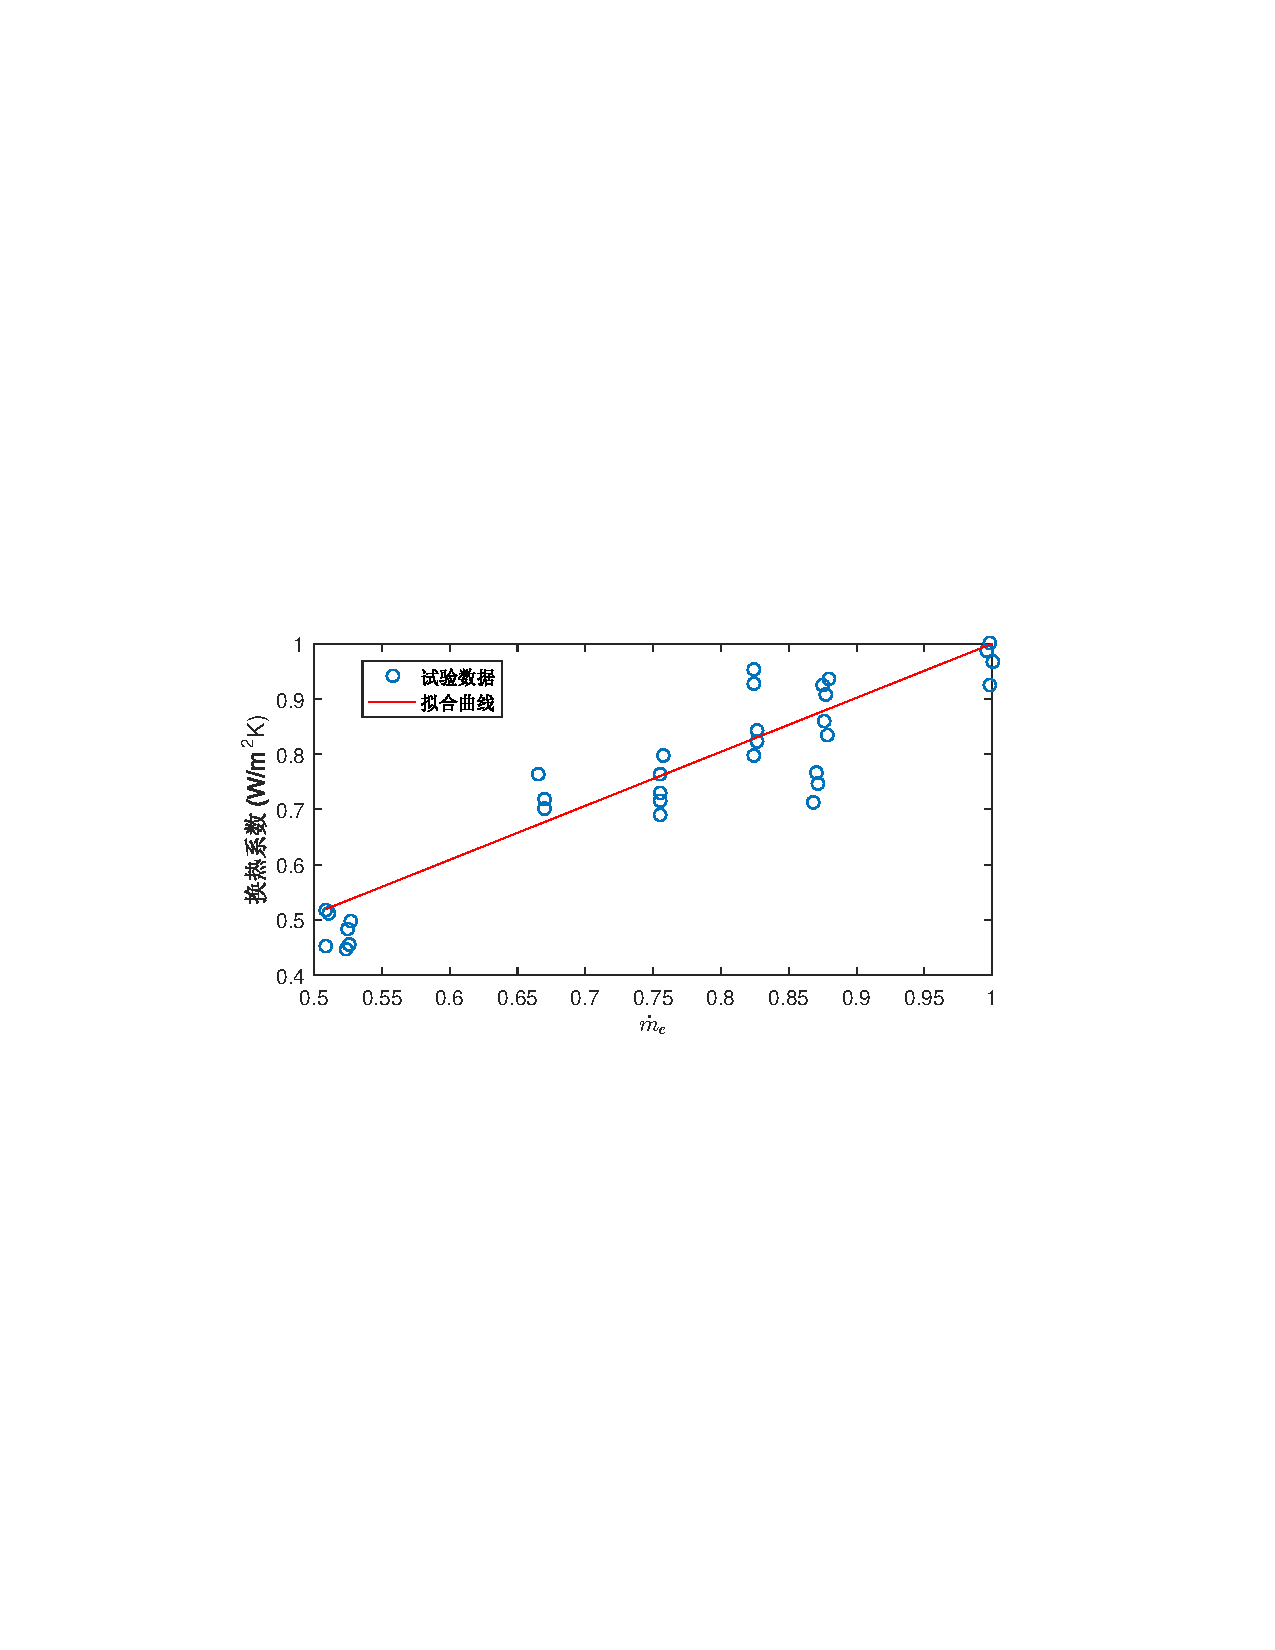
\includegraphics[scale=0.75]{figures/Chap1-7-HE-Part-Load.pdf}
  \caption{换热器换热系数的部分负载特性}
  \label{fig:HE-Part-Load}
\end{figure}

综上,换热器部分负载热力学模型包含的变量如表~\ref{tab:HE-comp-thermo-para}~所示,其边界条件如入口空气温度及压力均可由对应级的压缩机参数给定,同时空气侧质量流率与对应级压缩机的空气质量流率相同,因此其它变量可唯一给定。

\begin{table}[htb]
  \centering
  \begin{minipage}[t]{0.9\linewidth} % 如果想在表格中使用脚注,minipage是个不错的办法
  \caption{压缩侧换热器部分负载热力学模型变量表}
  \label{tab:HE-comp-thermo-para}
    \begin{tabularx}{\linewidth}{cccccc}
      \toprule[1.5pt]
      {\heiti 变量} & {\heiti 物理意义} & {\heiti 单位} &  {\heiti 变量} & {\heiti 物理意义} & {\heiti 单位} \\\midrule[1pt]
      $T_{c,HX,i}^{a,in}$ & 空气侧入口温度 & K  &  $T_{c,HX,i}^{a,out}$ & 空气侧出口温度 & K \\
      $T_{c,HX,i}^{HTF,in}$ & HTF侧入口温度 & K & $T_{c,HX,i}^{HTF,out}$ & HTF侧出口温度 & K \\
      $p_{c,HX,i}^{in}$ & 空气进口压力 & kPa & $p_{c,HX,i}^{out}$ & 空气出口压力 & kPa \\
      $\Phi _{c,i}^{HX}$ & 实际换热功率 & kW & ${\varepsilon _{c,i}}$ & 实际效能& ——  \\
      $NT{U_{c,i}}$ & 实际传热单元数 & —— & $C_{c,i}^{HX}$ &  实际热容比 &  —— \\
      $\eta _{c,HX,i}^p$ & 压力保持系数 & —— & $\dot m_c^{HTF}$ & 汇合后HTF流率 & kg/s\\
      $\dot m_{c,HX,i}^{HTF}$ & 载热流体流率 & kg/s & $C_{c,i}^{\max }$ & 最大热容 & kJ/s/K\\
      $C_{c,i}^{\min }$ & 最小热容 & kJ/s/K & $T_{c,HX}^{Merge}$ & 汇合后HTF温度 & K\\
      \bottomrule[1.5pt]
    \end{tabularx}
  \end{minipage}
\end{table}

\subsubsection{膨胀侧换热器}
定义第$i$ 级换热器的空气侧入口温度为 $T_{e,HX,i}^{a,in}$ ,HTF的入口温度为$T_{e,HX,i}^{HTF,in}$,则换热器出口侧空气温度及HTF温度分别为,
\begin{subequations}
\label{eq:he-turb-temp-out}
\begin{gather}
T_{e,HX,i}^{a,out} = T_{e,HX,i}^{a,in} + \Phi _{e,i}^{HX}/({c_p^a\dot m_e^a})\label{equ:he-turb-temp-air-out}\\
T_{e,HX,i}^{HTF,out} = T_{e,HX,i}^{HTF,in} - \Phi _{e,i}^{HX}/({c_p^{HTF}\dot m_{e,i}^{HTF}}) \label{equ:he-turb-temp-HTF-out}\\
\Phi _{e,i}^{HX} = {\varepsilon _{e,i}}C_{e,i}^{\min }({T_{e,HX,i}^{HTF,in} - T_{e,HX,i}^{a,in}})\label{equ:he-turb-thermal}
\end{gather}
\end{subequations}
其中,$\dot m_{e,i}^{HTF}$为膨胀侧第$i$级换热器的质量流率;$\Phi _{e,i}^{HX}$ 为换热器实际换热功率;${\varepsilon _{e,i}}$ 为换热器效能,对于图
\ref{fig:CAES-thermal-struc}中膨胀侧采用的逆流换热器,其效能为\cite{Heat-mass-transfer-11},
\begin{subequations}
\begin{gather}
{\varepsilon _{e,i}} = \frac{{1 - \exp [{- NT{U_{e,i}}({1 - C_{e,i}^{HX}})}]}}{{1 - C_{e,i}^{HX}\exp [{- NT{U_{e,i}}({1 - C_{e,i}^{HX}})}]}}\label{equ:he-eff-1}
%{\varepsilon _{e,i}} = \frac{{1 - \exp \left[ { - NT{U_{e,i}}\left( {1 + C_{e,i}^{HX}} \right)} \right]}}{{1 + C_{e,i}^{HX}}}\label{equ:he-turb-eff-2}
\end{gather}
\end{subequations}
其中,除下标$e$表示膨胀侧外,$NT{U_{e,i}}$ 与$C_{e,i}^{HX}$的含义与压缩侧换热器相同,且满足
\begin{subequations}
\begin{gather}
NT{U_{e,i}} = U_{e,i}A_{e,i}/C_{e,i}^{\min }, C_{e,i}^{HX} = C_{e,i}^{\min }/C_{e,i}^{\max }\label{equ:he-turb-NTU-C}\\
C_{e,i}^{\min } = {({{{\dot m}_e}c_p^a,\dot m_{e,i}^{HTF}c_p^{HTF}})_{\min }}\label{equ:he-turb-Cmin}\\
C_{e,i}^{\max } = {({{{\dot m}_e}c_p^a,\dot m_{e,i}^{HTF}c_p^{HTF}})_{\max }}\label{equ:he-turb-Cmax}
\end{gather}
\end{subequations}
其中, $C_{e,i}^{\max }$与$C_{e,i}^{\min }$的含义同压缩侧。

第$i$级换热器所需的换热介质的质量流率满足,
\begin{equation}
\label{equ:he-turb-mass-flow}
\dot m_{e,i}^{HTF} = \frac{{{{\dot m}_e}c_p^a({T_{e,HX,i}^{a,in} - T_{e,HX,i}^{a,out}})}}{{c_p^{HTF}({T_{e,HX,i}^{HTF,out} - T_{e,HX,i}^{HTF,in}})}}
\end{equation}

与压缩侧换热器类似,引入换热器压力保持系数\cite{Thesis-Lixuemei}后换热器的出口空气压力为,
\begin{subequations}
\begin{gather}
%\eta _{e,HX,i}^p = 1 - \frac{{0.0083{\varepsilon _{e,i}}}}{{1 - {\varepsilon _{e,i}}}}\label{equ:he-turb-pressure-discount}\\
p_{e,HX,i}^{out} = \eta _{e,HX,i}^pp_{e,HX,i}^{in}\label{equ:he-turb-pressure-out}
\end{gather}
\end{subequations}

此外,膨胀侧各级换热器汇合后的HTF质量流率及温度分别为,
\begin{subequations}
\begin{gather}
\dot m_e^{HTF} = \sum\limits_{i = 1}^{{N_e}} {\dot m_{e,i}^{HTF}} \label{equ:he-turb-mix-mass-flow}\\
T_{e,HX}^{Merge} = {{\sum\limits_{i = 1}^{{N_e}} {\dot m_{e,HX,i}^{HTF}T_{e,HX,i}^{HTF,out}} }}/{{\sum\limits_{i = 1}^{{N_e}} {\dot m_{e,HX,i}^{HTF}} }}\label{equ:he-turb-mix-temp}
\end{gather}
\end{subequations}

与压缩侧换热器类似,换热系数$U_{e,i}$随部分负载工况的变化明显,导致${\varepsilon _{e,i}}$ 及$\Phi _{e,i}^{HX}$的变化,从而影响透平膨胀机的入口空气温度。

综上,膨胀侧换热器部分负载热力学模型中的变量如表~\ref{tab:HE-turb-thermo-para}~所示,其边界条件如入口空气温度及压力均可由对应级的膨胀机参数给定,同时空气侧质量流率与对应级膨胀机的空气质量流率相同,因此相关其它变量可唯一给定。

\begin{table}[htb]
  \centering
  \begin{minipage}[t]{0.9\linewidth} % 如果想在表格中使用脚注,minipage是个不错的办法
  \caption{膨胀侧换热器部分负载热力学模型变量表}
  \label{tab:HE-turb-thermo-para}
    \begin{tabularx}{\linewidth}{cccccc}
      \toprule[1.5pt]
      {\heiti 变量} & {\heiti 物理意义} & {\heiti 单位} &  {\heiti 变量} & {\heiti 物理意义} & {\heiti 单位} \\\midrule[1pt]
      $T_{e,HX,i}^{a,in}$ & 空气侧入口温度 & K  &  $T_{e,HX,i}^{a,out}$ & 空气侧出口温度 & K \\
      $T_{e,HX,i}^{HTF,in}$ & HTF侧入口温度 & K & $T_{e,HX,i}^{HTF,out}$ & HTF侧出口温度 & K \\
      $p_{e,HX,i}^{in}$ & 空气进口压力 & kPa & $p_{e,HX,i}^{out}$ & 空气出口压力 & kPa \\
      $\Phi _{e,i}^{HX}$ & 实际换热功率 & kW & ${\varepsilon _{e,i}}$ & 实际效能& ——  \\
      $NT{U_{e,i}}$ & 实际传热单元数 & —— & $C_{e,i}^{HX}$ &  实际热容比 &  —— \\
      $\eta _{e,HX,i}^p$ & 压力保持系数 & —— & $\dot m_e^{HTF}$ &  汇合后HTF流率 & kg/s\\
      $\dot m_{e,HX,i}^{HTF}$ & 载热流体流率 & kg/s & $C_{e,i}^{\max }$ & 最大热容 & kJ/s/K\\
      $C_{e,i}^{\min }$ & 最小热容 & kJ/s/K & $T_{e,HX}^{Merge}$ & 汇合后HTF温度 & K\\
      \bottomrule[1.5pt]
    \end{tabularx}
  \end{minipage}
\end{table}

\subsection{能量存储类模块}
对AA-CAES各应用形式而言,一般均包含储热罐及储气库等能量存储类模块,本小节分别给出二者的热力学动态模型。

\subsubsection{储热罐}
\label{sec:TES-thermo-model}
根据压缩机级数及压缩机出口高压空气温度的不同,AA-CAES中压缩热能的存储可分为高温压缩热能存储(400$^{\circ}$C以上)~\cite{A-CAES-Dynamic-17,AA-CAES-07}、中温压缩热能存储(200$^{\circ}$C-400$^{\circ}$C)~\cite{ACAES-Packed-TES} 及低温压缩热能存储(200$^{\circ}$C以下)~\cite{TICC-16}等。相应地,储热技术的种类也较多~\cite{TES-CSP-review-13},AA-CAES各典型实现形式可采用的储热技术主要包括回热式双罐液态储热\cite{TICC-15}或填充床储热\cite{A-CAES-Dynamic-17}、混凝土储热\cite{Model-AA-CAES-10}及相变材料储热\cite{AA-CAES-Simulation-19}等方式。

本章针对常用的回热式双罐液态储热方式建立动态模型,该类储热方式已在我国多座AA-CAES试验系统中普遍使用,如TICC-500\cite{TICC-15}、STHC-100\cite{ST-CAES-17}以及江苏金坛AA-CAES国家示范电站\cite{CAES-Review-17-Rui-salt},同时也在集中式光热电站技术中广泛使用\cite{TES-CSP-review-13}。对于填充层储热结构,可采用文献~\inlinecite{A-CAES-Dynamic-17} 中的动态模型;对于蓄热式混凝土储热罐动态结构,可采用文献~\inlinecite{Model-AA-CAES-10} 中的动态模型;对于相变材料储热,其动态模型可参考文献~\inlinecite{AA-CAES-Simulation-19}。

%\subsubsection{双罐回热结构}
对于图~\ref{fig:CAES-thermal-struc}中所采用的双罐回热储热结构,低温储热罐一般通过与外界充分散热保持恒温,可视为等温;高温储热罐需尽可能减少传热损失,则高温储热罐中储热介质的温度满足,
%其储热模型可建立如下:
%\subsubsection{蓄热式储热结构}
%本章先探讨蓄热式混凝土储热罐动态模型,建模思路可推广至其他类型的储热系统的建模过程。考虑文献~\inlin%ecite{Model-AA-CAES-10}中的带沉浸式换热器线圈的储热系统,如图~\ref{fig:TES-struc-2}~所示。
%\begin{figure}[H] % use float package if you want it here
%  \centering
%  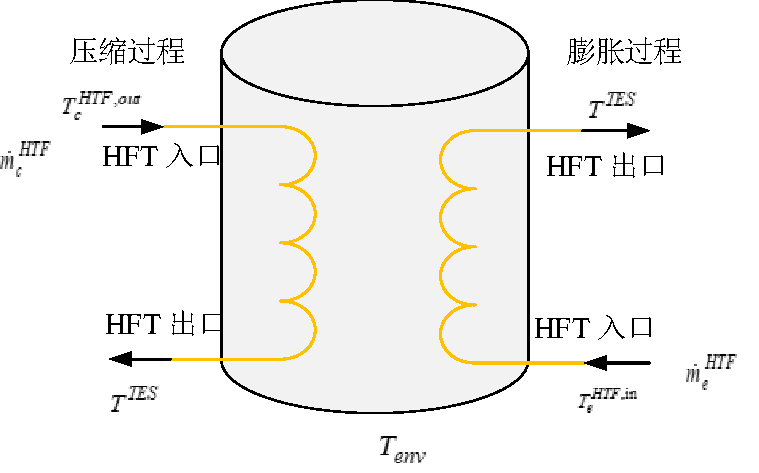
\includegraphics[scale=0.75]{Chap2-4-TES1-Structure}
%  \caption{带沉浸式换热线圈的储热系统示意图}
%  \label{fig:TES-struc-2}
%\end{figure}
\begin{equation}
\label{equ:TES-HTF-temp}
\begin{array}{l}
({{\rho _{TES}}{V_{TES}}c_p^{TES}})\frac{{d{T_{TES}}}}{{dt}} = \dot m_c^{HTF}c_p^{HTF}({T_{c,TES}^{HTF,in} - {T_{TES}}})\\
\;\;\;\;\;\;\;\;\;\;\;\;\;\;\;\;\;\;\;\;\;\;\;\;\; - \dot m_e^{HTF}c_p^{HTF}({{T_{TES}} - T_{e,TES}^{HTF,in}}) - {U_{TES}}{A_{TES}}({{T_{TES}} - {T_{env}}})
\end{array}
\end{equation}
其中,${\rho _{TES}}$ 为储热介质的密度;${V_{TES}}$ 为储热介质的体积;$c_p^{TES}$ 为储热介质的比热容;$T_{c,TES}^{HTF,in}$ 为压缩阶段HTF的出口温度,即$T_{c,HX}^{Merge}$;$T_{e,TES}^{HFT,in}$ 为膨胀阶段HTF的入口温度;${U_{TES}}$与${A_{TES}}$ 分别为储热罐与环境间的传热系数及储热罐的外部表面积,若不考虑传热损失,可令${U_{TES}}$为0;$T_{env}$ 为环境温度。一般情况下,储热介质可选用HTF(如TICC-500采用加压水),也可不同于HTF(如集中式光热电站),本文假定储热介质选用HTF。

\subsubsection{储气库}
\label{sec:Air-tank-thermo-model}
~AA-CAES~可采用的储气方式主要包括压力控制型(即等压储气库)\cite{Isobaric-ACAES-18,Thesis-Wangzhiwen}与容积控制型(即等容储气库)\cite{TICC-15,Thesis-JaiDuhan}两种。本文重点关注较为常见且对地理条件依赖性较小的容积控制型储气库,包括压力容器\cite{TICC-15}、盐穴储气\cite{CAES-Review-17-Rui-salt}、管线钢\cite{ST-CAES-CN-16-Rui}等,如图~\ref{fig:CAES-thermal-struc}中采用的储气库。对于容积控制型储气库,大多研究假定储气库为恒温,如文献~\inlinecite{CAES-Discharge-16}基于恒温储气库模型,研究了D-CAES的两种膨胀侧运行模式;文献~\inlinecite{CAES-CCHP-off-design-18} 基于恒温储气库模型研究了基于AA-CAES的CCHP系统的不同运行模式。然而,实际过程中随着压缩与膨胀过程中高压空气的注入及排出,以及储气库与周围环境之间的换热量的变化,储气库内空气的压力及温度均会发生变化,从而影响压缩储能过程中末级压缩机背压(无入口侧节流阀时)与膨胀释能过程中透平入口空气温度及压力(无出口侧节流阀时)等热力学参数。为此,本文基于文献~\inlinecite{Model-AA-CAES-10} 及文献~\inlinecite{Cavern-model-12}中的温度与压力动态模型,建立储气库通用热力学仿真模型。

\textbf{(1)通用定容模型}

通用定容模型(记为G模型)假定储气库内空气的温度与压力均随压缩储能及膨胀释能过程变化,同时计及储气库与周围环境的换热过程。如此,通用定容储气库的热力学动态模型为\cite{Model-AA-CAES-10,Cavern-model-12},
\begin{subequations}
\label{equ:Air-tank-model-G}
\begin{gather}
   \frac{{d{m_{as}}}}{{dt}} = \dot m_{as}^{in} - \dot m_{as}^{out}\\
   \frac{{d{T_{as}}}}{{dt}} = \frac{1}{{{m_{as}}}}[ {({1 - \frac{1}{k}})({\dot m_{as}^{in}T_{as}^{in} - \dot m_{as}^{out}T_{as}^{}})} ] + \frac{{{\alpha _w}{A_w}({{T_w} - {T_{as}}})}}{{{m_{as}}c_p^a}}\label{equ:Air-tank-model-G-T}\\
   \frac{{d{p_{as}}}}{{dt}} = \frac{{k{R_g}}}{{{V_{as}}}}({\dot m_{as}^{in}T_{as}^{in} - \dot m_{as}^{out}T_{as}^{}}) + \frac{{{R_g}}}{{c_v^a{V_{as}}}}{\alpha _w}{A_w}({{T_w} - {T_{as}}} )\label{equ:Air-tank-model-G-P}
\end{gather}
\end{subequations}
其中,${m_{as}}$ 为储气库中的高压空气质量;$\dot m_{as}^{in}$ 与$\dot m_{as}^{out}$分别为储气库的进口空气质量流率与出口空气质量流率;$T_{as}^{in}$与 $T_{as}$ 分别为储气库的进口空气温度与出口空气温度(或储气库的实时空气温度);${A_w}$ 为储气库与周围环境的接触面积; ${T_w}$ 为储气库壁面温度,可采用一维热传导方程求解;$p_{as}(t)$为储气库空气压力;$R_g$为通用气体常数;${\alpha _w}$ 为储气库外表面与环境间的传热系数,其值与储气库的特性有关,如文献~\inlinecite{CAES-Huntorf-12}基于实测Huntorf 电站数据仿真拟合得到了适用于地下盐穴储气库的可变传热系数,
\begin{equation}
\label{equ:wall-thermal-coef}
{\alpha _w} = 0.02356 + 0.0149{\left| {\dot m_{as}^{in} - \dot m_{as}^{out}} \right|^{0.8}}
\end{equation}

事实上,储气库内空气的实时压力$p_{as}$亦可基于空气温度$T_{as}$和质量$m_{as}$,并结合理想气体状态方程求解,即(\ref{equ:Air-tank-model-G}) 存在冗余项。为了描述壁面换热对储气库内空气的热力学特性(温度及压力)的影响,此处给出了二者的具体表达式。从温度动态方程(\ref{equ:Air-tank-model-G-T})及压力动态方程(\ref{equ:Air-tank-model-G-P})可知,储气库(出口)空气温度受进出口空气质量流率及储气库与周围环境的传热过程共同影响,在较大质量流率充气与放气过程中,前者对储气库内空气温度与压力的变化影响较大;在较小质量流率充放气过程中,如压缩机与膨胀机部分负载运行时,储气库与周围环境的传热过程对储气库内空气温度与压力的变化贡献较大,这一现象已在基于盐穴储气的Huntorf D-CAES电站实际运行中得到验证\cite{Huntorf-20-01}。 因此,在研究AA-CAES宽工况热力学仿真模型时,通用储气库模型应考虑储气库与周围环境的传热过程。

\textbf{(2)定容等温与绝热模型}

对于非地下盐穴储气等其它小型储气方式而言,储气罐(库)与罐(库)壁的传热损失并不明显,或可通过易于实现的保温、绝热等方式加以控制,此时可在通用定容模型的基础上,进一步简化得到定容等温模型与定容绝热模型。定容等温模型(记为VT模型)假设储气库内空气的温度不随时间变化,从而储气库G模型退化为,
\begin{subequations}
\label{equ:Air-tank-model-VT}
\begin{gather}
    \frac{{d{m_{as}}}}{{dt}} = \dot m_{as}^{in} - \dot m_{as}^{out}\\
    \frac{{d{T_{as}}}}{{dt}} = 0\\
    \frac{{d{p_{as}}}}{{dt}} = \frac{{k{R_g}}}{{{V_{as}}}}( {\dot m_{as}^{in}T_{as}^{in} - \dot m_{as}^{out}T_{as}^{}})
\end{gather}
\end{subequations}

类似地,定容绝热储气库模型(记为VA模型)可表示为,
\begin{subequations}
\label{equ:Air-tank-model-VA}
\begin{gather}
    \frac{{d{m_{as}}}}{{dt}} = \dot m_{as}^{in} - \dot m_{as}^{out}\\
    \frac{{d{T_{as}}}}{{dt}} = \frac{1}{{{m_{as}}}}[ {({1 - \frac{1}{k}})({\dot m_{as}^{in}T_{as}^{in} - \dot m_{as}^{out}T_{as}^{}} )} ]\\
    \frac{{d{p_{as}}}}{{dt}} = \frac{{k{R_g}}}{{{V_{as}}}}({\dot m_{as}^{in}T_{as}^{in} - \dot m_{as}^{out}T_{as}^{}})
\end{gather}
\end{subequations}


\textbf{(3) 储气库壁面温度求解}

通用定容储气库模型(\ref{equ:Air-tank-model-G})中,$T_{as}$ 及$p_{as}$的求解需要获取墙壁温度$T_w$。$T_w$随储气库内高压空气温度的不同而变化,具体可通过求解一维热传导方程获得\cite{Heat-mass-transfer-11}。如图~\ref{fig:cavern-wall-temp} 所示,定义储气库与墙壁周边任一截面上的温度为$T_{rs}$,由一维热传导方程可得任一时刻任一位置处的温度为~\cite{Heat-mass-transfer-11,Model-AA-CAES-10,Cavern-wall-09},
\begin{equation}
\label{eq:wall-temp}
\frac{{\partial {T_{rs}}\left( {t,r} \right)}}{{\partial t}} = {r_{rs}}({\frac{{{\partial ^2}{T_{rs}}}}{{\partial {r^2}}} + \frac{1}{r}\frac{{\partial {T_{rs}}}}{{\partial r}}})
\end{equation}
其中,${r_{rs}}$为墙壁与储气库的热扩散率。

\begin{figure}[H] % use float package if you want it here
  \centering
  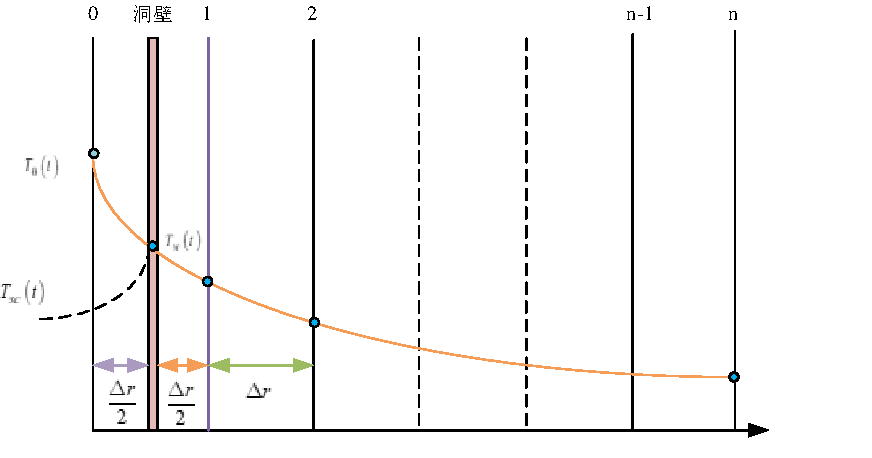
\includegraphics[scale=0.8]{Chap2-5-Wall-Temperature}
  \caption{储气库与洞穴壁温度分布示意图}
  \label{fig:cavern-wall-temp}
\end{figure}

通过求解热传导方程(\ref{eq:wall-temp})的空间离散化方程组(具体求解过程参见附录~\ref{cha:air-wall-temp-exp}),可获取洞穴壁的温度,
\begin{equation}
{T_w}(t) = \frac{{{T_{rs,1}}(t) + {T_{rs,0}}(t)}}{2} = \frac{{{T_{sc,a}}}}{{2({\frac{1}{{B{i^ + }}} + \frac{1}{2}})}} + {T_{rs,1}}({1 - \frac{1}{{({\frac{1}{{B{i^ + }}} + \frac{1}{2}})}}})
\end{equation}
其中,毕奥数(Biot-number) $B{i^ + } = \frac{{{\alpha _{a,w}}\Delta r}}{{{r_{rs}}}}$,${\alpha _{a,w}}$ 表示从空气到洞穴壁的传热系数。

综上,储气库模块的热力学动态模型中的变量如表~\ref{tab:Air-tank-thermo-para}~所示。
\begin{table}[htb]
  \centering
  \begin{minipage}[t]{0.9\linewidth} % 如果想在表格中使用脚注,minipage是个不错的办法
  \caption{储气库热力学动态模型变量表}
  \label{tab:Air-tank-thermo-para}
    \begin{tabularx}{\linewidth}{cccccc}
      \toprule[1.5pt]
      {\heiti 变量} & {\heiti 物理意义} & {\heiti 单位} &  {\heiti 变量} & {\heiti 物理意义} & {\heiti 单位} \\\midrule[1pt]
      ${m_{as}}$ & 储气库中高压空气质量 & Kg  &  $\dot m_{as}^{in}$ & 储气库进口空气流率 & Kg/s \\
      $\dot m_{as}^{out}$ & 储气库出口空气流率 & Kg/s & $T_{as}^{in}$ & 储气库进口空气温度 & K \\
      $T_{as}^{out}/T_{as}$ & 储气库出口空气温度 & K & ${T_w}$ & 墙壁温度 & K \\
      ${p_{as}}$ & 储气库空气实时压力 & kPa & & &\\
      \bottomrule[1.5pt]
    \end{tabularx}
  \end{minipage}
\end{table}

\subsection{运行模式控制模块}
\label{sec:part-load-energy-TV}

AA-CAES四种运行模式的确定可由运行模式控制模块,即储气库入口侧的节流阀及储气库出口侧的节流阀来控制,本小节给出其热力学模型。

一般而言,绝热节流是等焓过程~\cite{Eng-Thermo-83},节流前后空气质量流率相同,温度相同,只有压力不同。因此,流经储气库入口侧节流阀(Throttle Valve, TV)模块的空气满足,
\begin{equation}
    \dot m_{c,TV}^{in} = \dot m_{c,TV}^{out}, T_{c,TV}^{in} = T_{c,TV}^{out}
\end{equation}
节流前后空气的压力由其它边界条件确定。

类似地,流经储气库出口侧的节流阀模块的空气满足,
\begin{equation}
    \dot m_{e,TV}^{in} = \dot m_{e,TV}^{out}, T_{e,TV}^{in} = T_{e,TV}^{out}
\end{equation}
%节流前后压力亦由其它边界条件确定。

综上,节流阀模块热力学模型中的变量如表~\ref{tab:throttle-valve-para}~所示。
\begin{table}[htb]
  \centering
  \begin{minipage}[t]{0.88\linewidth} % 如果想在表格中使用脚注,minipage是个不错的办法
  \caption{节流阀热力学模型变量表}
  \label{tab:throttle-valve-para}
    \begin{tabularx}{\linewidth}{cccccc}
      \toprule[1.5pt]
      {\heiti 变量} & {\heiti 物理意义} & {\heiti 单位} &  {\heiti 变量} & {\heiti 物理意义} & {\heiti 单位} \\\midrule[1pt]
      $\dot m_{c,TV}^{in}$ & 压缩侧TV入口流率 & kg/s &  $\dot m_{c,TV}^{out}$ & 压缩侧TV出口流率 & kg/s \\
      $T_{c,TV}^{in}$ & 压缩侧TV入口温度 & K & $T_{c,TV}^{out}$ & 压缩侧TV出口温度 & K \\
      $p_{c,TV}^{in}$ & 压缩侧TV入口压力 & kPa & $p_{c,TV}^{out}$ & 压缩侧TV出口压力 & kPa \\
      $\dot m_{e,TV}^{in}$ & 透平侧TV入口流率 & kg/s &  $\dot m_{e,TV}^{out}$ & 透平侧TV出口流率 & kg/s \\
      $T_{e,TV}^{in}$ & 透平侧TV入口温度 & K & $T_{e,TV}^{out}$ & 透平侧TV出口温度 & K \\
      $p_{e,TV}^{in}$ & 透平侧TV入口压力 & kPa & $p_{e,TV}^{out}$ & 透平侧TV出口压力 & kPa \\
      \bottomrule[1.5pt]
    \end{tabularx}
  \end{minipage}
\end{table}

\subsection{模型边界条件及性能指标}
\label{sec:part-load-energy-boundary}
边界条件定义了AA-CAES各组件模型之间的关联关系,主要包括压缩侧接口与膨胀侧接口。以下针对图~\ref{fig:CAES-thermal-struc}所示的AA-CAES结构给出其边界条件,其它AA-CAES结构可稍作修改即可。

\subsubsection{压缩侧模型接口}
第$i$级压缩机的入口空气温度与压力分别为环境压力$p_0$与环境温度$T_0$。第$i$级($1\le i<N_c$)压缩机的出口空气温度与压力为第$i$级压缩侧换热器的入口空气温度与压力,第$i$ 级换热器的出口空气压力与温度为第$i+1$级压缩机的入口空气压力与温度,即
\begin{subequations}
\begin{gather}
T_{c,HX,i}^{a,in} = T_{c,i}^{out},T_{c,HX,i}^{a,out} = T_{c,i + 1}^{in},\;\forall 1\le i < {N_c}\\
p_{c,HX,i}^{a,in} = p_{c,i}^{out},p_{c,HX,i}^{a,out} = p_{c,i + 1}^{in},\;\forall 1\le i < {N_c}
%{{\dot m}_c} = \dot m_{as}^{in}
\end{gather}
\end{subequations}

整个压缩侧经过各级压缩机、换热器及节流阀的空气质量流率相同。同时,末级压缩机($i=N_c$)的出口空气压力与温度分别为末级换热器的入口空气压力与温度,末级换热器的出口空气压力与温度则视AA-CAES压缩侧运行模式而不同。具体为:1)压缩侧常压运行模式下,
\begin{subequations}
\begin{gather}
\dot m_{c,TV}^{in} = {{\dot m}_c},\dot m_{c,TV}^{out} = \dot m_{as}^{in}\\
T_{c,HX,i}^{a,in} = T_{c,i}^{out},T_{c,HX,i}^{a,out} = T_{c,TV}^{in},T_{c,TV}^{out} = T_{as}^{in}\;,i = {N_c}\\
p_{c,HX,i}^{a,in} = p_{c,i}^{out},p_{c,HX,i}^{a,out} = p_{as}^{\max },\;p_{c,TV}^{in} = p_{as}^{\max },p_{c,TV}^{out} = p_{as}^{},i = {N_c}
\end{gather}
\end{subequations}
2)压缩侧滑压模式下,
\begin{subequations}
\begin{gather}
{{\dot m}_c} = \dot m_{as}^{in}\\
T_{c,HX,i}^{a,in} = T_{c,i}^{out},T_{c,HX,i}^{a,out} = T_{as}^{in}\;,i = {N_c}\\
p_{c,HX,i}^{a,in} = p_{c,i}^{out},p_{c,HX,i}^{a,out} = p_{as}^{},\;i = {N_c}
\end{gather}
\end{subequations}
其中,$p_{as}^{max}$为储气库最大工作压力。

第$i$级($1\le i\le {N_c}$)换热器载热流体的入口温度均为定值,为冷罐中的HTF温度,即
\begin{equation}
T_{c,HX,i}^{HTF,in} = T_{cool}^{HTF}
\end{equation}
所有换热器载热流体侧出口温度汇合后的温度为储热罐的入口HTF 温度,即
\begin{equation}
T_{c,HX}^{HTF,Merge} = T_{c,TES}^{HTF,in}
\end{equation}

\subsubsection{膨胀侧模型接口}
第$i$级($1<i\le N_e$)膨胀机的入口空气温度与压力分别为第$i$级膨胀机侧换热器的出口空气温度与压力,第$i$级( $1<i\le N_e$)换热器的入口空气压力与温度分别为第$i-1$ 级膨胀机的出口空气压力与温度,即
\begin{subequations}
\begin{gather}
T_{e,HX,i}^{a,out} = T_{e,i}^{in},T_{e,HX,i}^{a,in} = T_{e,i + 1}^{out},\;\forall 1<i\le N_e\\
p_{e,HX,i}^{a,out} = p_{e,i}^{in},p_{e,HX,i}^{a,in} = p_{e,i + 1}^{out},\;\forall 1<i\le N_e
%{{\dot m}_e} = \dot m_{as}^{out}
\end{gather}
\end{subequations}

整个膨胀侧流经节流阀、各级换热器、膨胀机的空气质量流率相同。同时,首级膨胀机的入口空气压力与温度分别为首级换热器的出口空气压力与温度,首级换热器的入口空气压力与温度则视AA-CAES膨胀侧运行模式而不同。具体地:1)膨胀侧常压运行模式下,
\begin{subequations}
\begin{gather}
\dot m_{e,TV}^{out} = {{\dot m}_e},\dot m_{e,TV}^{in} = \dot m_{as}^{out}\\
T_{e,HX,i}^{a,out} = T_{e,i}^{in},T_{e,HX,i}^{a,in} = T_{e,TV}^{out},T_{e,TV}^{in} = T_{as}\;,i = 1\\
p_{e,HX,i}^{a,out} = p_{e,i}^{in},p_{e,HX,i}^{a,in} = p_{as}^{\min },\;p_{e,TV}^{out} = p_{as}^{\min },p_{e,TV}^{in} = p_{as}^{},i = 1
\end{gather}
\end{subequations}
2)膨胀侧滑压运行模式下,
\begin{subequations}
\begin{gather}
{{\dot m}_e} = \dot m_{as}^{out}\\
T_{e,HX,i}^{a,out} = T_{e,i}^{in},T_{e,HX,i}^{a,in} = T_{as}^{out}\;,i = 1\\
p_{e,HX,i}^{a,out} = p_{e,i}^{in},p_{e,HX,i}^{a,in} = p_{as}^{out},\;i = 1
\end{gather}
\end{subequations}
其中,$p_{as}^{min}$为储气库最小工作压力。

第$i$级($1\le i\le N_e$)换热器载热流体的入口温度均为定值,为储热罐的HTF出口温度,即
\begin{equation}
T_{e,HX,i}^{HTF,in} = {T_{e,TES}^{HTF,in}}
\end{equation}
所有换热器载热流体侧的出口HTF温度汇合后的温度为冷罐中的HTF 温度,即
\begin{equation}
T_{e,HX}^{HTF,Merge} = T_{cool}^{HTF}
\end{equation}
此外,第$N_e$级膨胀机排气压力需大于$p_0$, 排气温度可视温度的大小,可用于制冷或供暖。

\subsubsection{能量效率指标}
\label{sec:part-load-energy-full}
%本章一定要考虑电动机与发电机的效率,为直接实现第5章机械转矩或机械功的输入或输出建模埋下伏笔与奠定基础。
基于组件级的部分负载热力学模型,可构建AA-CAES系统级的通用宽工况热力学仿真模型,具体包括压缩机、空气透平及换热器的部分负载热力学模型,储热罐与储气库的热力学动态模型,节流阀模型及受控于AA-CAES运行方式的边界条件。

为了分析AA-CAES系统级的性能,定义电效率、热效率及总能利用系数分别为,
\begin{equation}
%{\eta _{work}} = \frac{{{\int_0^{t_{dis}}W_e}}}{{{\int_0^{t_{ch}}W_c}}}, {\eta _{hot}} = \frac{{Q_H^L}}{{\int_0^{t_{ch}}{W_c}}}, {\eta _{cool}} = \frac{{Q_C^L}}{{{\int_0^{t_{ch}}W_c}}}
{\eta _{elec}} = \frac{{\int_0^{{t_{dis}}} {{W_e}dt}}}{{{\int_0^{{t_{ch}}} {{W_c}dt}}}}, {\eta _{heat}} = \frac{{Q_H^L}}{{{\int_0^{{t_{ch}}} {{W_c}dt}}}}, {\eta _{total}} = {\eta _{elec}} + {\eta _{heat}}
\end{equation}
%3)定义体积储能密度为
%\begin{equation}
%EVR = \frac{{{E_e}}}{{{V_{as}}}} = %\frac{{\int_0^{{t_{dis}}} {{{W_{e}}}dt} %}}{{{V_{as}}}}
%\end{equation}
其中,$t_{ch}$与$t_{dis}$分别为压缩储能时间与膨胀释能时间;$Q_{H}^{L}$为一个循环周期内AA-CAES对外提供的热能,其具体计算方式视AA-CAES系统结构、供热方式等的不同而异。%本文将在后续针对具体的系统分析中给出其对应的定义。

\section{基于㶲平衡的宽工况热力学模型}
\label{sec:chap2-part-load-exergy}
AA-CAES具有典型的多能流耦合特性,主要表现为对内的空气压缩热能与压力势能双能流间的耦合,以及对外的冷、热、电多能流间的耦合。基于热平衡的宽工况仿真模型难以从统一的视角给出AA-CAES内外多能流间的差异,而基于㶲理论的思路可为分析AA-CAES的多能流特性提供新的视角,本节将给出基于㶲平衡的仿真模型。 事实上,通过第
\ref{sec:part-load-energy}节的热力学仿真模型可以得到AA-CAES宽工况运行时各组件在额定工况或部分负载工况下作功工质(空气、HTF)在各热力学状态点(如图
\ref{fig:CAES-thermal-struc} 中标注的状态点1-12 及$1^*$-$14^*$)的流率、压力、温度等参数,并基于此通过查询工质(空气、HTF等)的热物性表\footnote{热物性表可利用NIST的REFPROP获取,具体可参见https://www.nist.gov/srd/refprop},即可得到对应状态点下的焓值及熵值~\cite{Eng-Thermo-83},进而可建立AA-CAES的㶲平衡模型。

\subsection{压缩机㶲模型}
压缩机的输入㶲为消耗的压缩功,输出㶲为入口与进口空气焓㶲差。如此,第$i$级压缩机的输入㶲与输出㶲分别为\cite{Eng-Thermo-83},
\begin{subequations}
\label{eq:exergy-compressor}
\begin{gather}
Ex_{c,i}^{in} = {W_{c,i}}\label{equ:comp-exergy-in}\\
Ex_{c,i}^{out} = {\dot m_c}[ {c_p^a\left( {T_{c,i}^{out} - T_{c,i}^{in}} \right) - {T_0}({c_p^a\ln \frac{{T_{c,i}^{out}}}{{T_{c,i}^{in}}} - {R_g}\ln \frac{{p_{c,i}^{out}}}{{p_{c,i}^{in}}}})}]\label{equ:comp-exergy-out}
\end{gather}
\end{subequations}

相应地,第$i$级压缩机的㶲损为,
\begin{equation}
\label{equ:comp-exergy-loss}
L{x_{c,i}} = Ex_{c,i}^{in} - Ex_{c,i}^{out}
\end{equation}

\subsection{空气透平㶲模型}
透平的输入㶲由空气提供,输出㶲为输出功。如此,进入第$i$级空气透平的输入㶲与输出㶲分别为\cite{Eng-Thermo-83},
\begin{subequations}
\begin{gather}
Ex_{e,i}^{in} = {\dot m_e}[ {c_p^a( {T_{e,i}^{in} - T_{e,i}^{out}}) - {T_0}({c_p^a\ln \frac{{T_{e,i}^{in}}}{{T_{e,i}^{out}}} - {R_g}\ln \frac{{p_{e,i}^{in}}}{{p_{e,i}^{out}}}})}]\label{equ:turb-exergy-in}\\
Ex_{e,i}^{out} = {W_{e,i}}\label{equ:turb-exergy-out}
\end{gather}
\end{subequations}

相应地,第$i$级膨胀机的㶲损为,
\begin{equation}
\label{equ:turb-exergy-loss}
L{x_{e,i}} = Ex_{e,i}^{in} - Ex_{e,i}^{out}
\end{equation}

\subsection{换热器㶲模型}

\textbf{(1)压缩侧换热器}

压缩侧换热器的输入㶲由高温空气提供,输出㶲由载热流体带走。如此,进入第$i$级换热器的㶲为,
\begin{equation}
\label{equ:he-comp-exergy-in}
Ex_{HX,i}^{c,in} = {\dot m_c}[ {c_p^a({T_{HX,i}^{a,in} - T_{HX,i}^{a,out}}) - {T_0}c_p^a\ln \frac{{T_{HX,i}^{a,in}}}{{T_{HX,i}^{a,out}}}}]
\end{equation}

流出第$i$级换热器的㶲为载热流体带走的㶲,即
\begin{equation}
\label{equ:he-comp-exergy-out}
Ex_{HX,i}^{c,out} = \dot m_{c,i}^{HTF}\left[ {({h_{HX,i}^{HTF,out} - h_{HX,i}^{HTF,in}}) - {T_0}({s_{HX,i}^{HTF,out} - s_{HX,i}^{HTF,in}})}\right]
\end{equation}
其中,$h_{HX,i}^{HTF,in}$与$s_{HX,i}^{HTF,in}$分别为换热器HTF侧的入口焓与熵;$h_{HX,i}^{HTF,out}$与$s_{HX,i}^{HTF,out}$分别为出口焓与熵;$h_{0}^{HTF}$与$s_{0}^{HTF}$分别为参考点的焓与熵\footnote{一般而言,AA-CAES系统中空气、HTF等稳流工质的㶲均需由焓($h$)与熵($s$) 计算。由于本文假设空气为理想气体,其$h$, $s$ 均为温度的单变量函数,故采用温度表示了空气的熵与焓,如(\ref{equ:he-comp-exergy-in}); 而HTF由于种类多,具体类型视特定系统而定,可采用加压水、导热油、熔融盐等,一般不是理想工质,故直接用$h$ 与$s$表示,如(\ref{equ:he-comp-exergy-out})。}。

相应地,第$i$级换热器的㶲损为,
\label{equ:he-comp-exergy-loss}
\begin{equation}
Lx_{HX,i}^c = Ex_{HX,i}^{c,in} - Ex_{HX,i}^{c,out}
\end{equation}

\textbf{(2)膨胀侧换热器}

与压缩侧换热器相反,膨胀侧换热器的输入㶲由高温HTF提供,输出㶲由空气带走。如此,流入第$i$级换热器的输入㶲为,
\begin{equation}
\label{equ:he-turb-exergy-in}
Ex_{HX,i}^{e,in} = \dot m_{e,i}^{HTF}\left[{({h_{HX,e,i}^{HTF,in} - h_{HX,e,i}^{HTF,out}}) - {T_0}({s_{HX,e,i}^{HTF,in} - s_{HX,e,i}^{HTF,out}})}\right]
\end{equation}
其中,相关变量的含义同压缩侧换热器,下标$e$表示膨胀侧。

流出第$i$级换热器的㶲为空气带走的㶲,即
\begin{equation}
\label{equ:he-turb-exergy-out}
Ex_{HX,i}^{e,out} = {\dot m_{e,i}}[ {c_p^a({T_{HX,i}^{a,e,out} - T_{HX,i}^{a,e,in}}) - {T_0}c_p^a\ln \frac{{T_{HX,i}^{a,e,out}}}{{T_{HX,i}^{a,e,in}}}}]
\end{equation}

相应地,第$i$级换热器的㶲损为,
\begin{equation}
\label{equ:he-turb-exergy-loss}
Lx_{HX,i}^e = Ex_{HX,i}^{e,in} - Ex_{HX,i}^{e,out}
\end{equation}

\subsection{节流阀㶲模型}
 节流阀的输入㶲为入口空气的㶲,输出㶲为出口空气的㶲。对于入口侧节流阀而言,输入㶲为末级换热器的出口空气㶲,输出㶲为进入储气库前的高压空气的焓㶲。因此,储气库入口侧及出口侧节流阀的㶲损分别为,
\begin{subequations}
\label{eq:exergy-TV}
\begin{gather}
Lx_{TV}^c = Ex_{c,TV}^{in} - Ex_{c,TV}^{out} \label{equ:throttle-valve-comp-exergy-loss}\\
Lx_{TV}^e = Ex_{e,TV}^{in} - Ex_{e,TV}^{out} \label{equ:throttle-valve-turb-exergy-loss}
\end{gather}
\end{subequations}
其中,$Ex_{c,TV}^{in}$为压缩侧末级换热器出口空气的焓㶲;$Ex_{c,TV}^{out}$为储气库入口侧空气的焓㶲;$Ex_{e,TV}^{in}$为储气库出口侧空气的焓㶲; $Ex_{e,TV}^{out}$为膨胀侧首级换热器入口空气的焓㶲;四者均可由对应空气的热力学状态参数(温度、压力)计算得出。
%\begin{equation}
%Ex = \dot mc_p^a\left( {T - {T_0}\ln T} %\right)
%\end{equation}

%\subsection{储气库㶲模型}

%\subsection{储热罐㶲模型}

\subsection{㶲效率指标}
基于热力学第一定律的性能指标可以反映系统内的能量转换情况,但其将功与热等同对待,导致该类效率评价指标只能反映系统能量利用的数量关系,不能反映其在能量利用品位上的不同,难以应用于AA-CAES多能联供应用场景的分析。为此,定义基于热力学第二定律的㶲效率指标以分析系统性能。

基于㶲的电效率、热效率及总㶲效率分别为,
\begin{equation}
{\eta _{x,elec}} = \frac{{\int_0^{{t_{dis}}} {Ex_e^{out}dt} }}{{\int_0^{{t_{ch}}} {Ex_c^{in}dt} }},{\eta _{x,heat}} = \frac{{Ex_H^L}}{{\int_0^{{t_{ch}}} {Ex_c^{in}dt} }}, {\eta _x} = {\eta _{x,elec}} + {\eta _{x,heat}}
\end{equation}
其中,${Ex_H^L}$为AA-CAES多能联供的热量㶲。

%为分析方便,引入储气库的㶲存储能力~\cite{Exergy-storage-17},
%\begin{equation}
%Ex_{as}^{\max } = \int_0^{{t_{ch}}} %{\dot E{x_{as}}dt}  = \int_0^{{t_{ch}}} %{{{\dot m}_c}\left\{ {c_p^a\left( %{{T_{as}^{in}} - {T_0}} \right) - %{T_0}\left[ {c_p^a\ln \left( %{\frac{T_{as}}{{{T_0}}}} \right) - R\ln %\left( {\frac{p_{as}}{{{p_0}}}} %\right)} \right]} \right\}dt}
%\end{equation}

%此外,在多能联供场景下,定义制热能效比与制冷能效比
%\begin{equation}
%CO{P_h} = \frac{{Q_H^L}}{{\int_0^{t_{ch%}}{W_cdt} - \int_0^{t_{dis}}{W_edt}}}, %CO{P_c} = \frac{{Q_{\rm{C}}^{\rm{L}}}}{%{\int_0^{t_{ch}}{W_cdt} - %\int_0^{t_{dis}}{W_edt}}}
%\end{equation}
%其中,$\int_0^{t_{ch}}{W_cdt} - \int_0^{t_{dis}}{W_edt}$ 等效表示系统生产热能与冷能所消耗的机械功。

\section{宽工况仿真平台实现及典型系统热力学特性分析}
\label{sec:chap2-bound-measure}

\subsection{宽工况仿真系统的实现}
第\ref{sec:part-load-energy}节中压缩机及空气透平的部分负载热力学模型中引入了压缩机转速$n_c$与透平转速$n_e$,二者分别由与之相连的电动机与发电机的转速及对应的转速控制策略决定。考虑到Matlab/Simulink自带了电力系统仿真模块SIMPOWER,其中的发电机与电动机模块设有转速接口,可直接与本章的压缩机与膨胀机的热力学模型集成。同时,本文第1.2节提出的接口灵活性需挖掘压缩机与膨胀机的机械输入与输出接口,而非电能输入与电能输出接口。因此,为了AA-CAES宽工况仿真模型与电力系统接口的功能拓展以及仿真系统的通用性,本节基于Matlab/Simulink构建如图~\ref{fig:Simulation-Platform} 所示的计及组件部分负载特性的AA-CAES宽工况热力学仿真系统,主要包括压缩机模块(内置压缩侧换热器)、膨胀机模块(内置膨胀侧换热器)、储气库模块、储热罐模块、节流阀模块以及功能控制模块,各模块实现本章所构建的热力学模型及对应的接口条件\footnote{模型中的㶲计算采用了开源Matlab㶲接口程序HOT(Thermodynamic Tools for Matlab),具体可参见http://hot-tdb.sourceforge.net/}。

事实上,正如第\ref{sec:research-state}节分析的AA-CAES的灵活性一样,在不同的结构实现形式中AA-CAES与电力/热力的接口不同,相应的转速控制策略也有所不同,但一般均会采用最优转速控制策略,实现高效运行。为便于分析方便,本节假定实际AA-CAES 实时通过转速$n_c$与$n_e$的调节确保了压缩机与膨胀机在相应运行工况下的最大等熵效率运行,即图\ref{fig:Comp-Ratio-off-design}与图\ref{fig:Eff-part-load} 中的压比与等熵效率可分别表示为质量流率的单值函数,膨胀机与之类似。
%为此,参考热力学仿真工具包Thermolib中的设置方式,得到如下的四组通用压缩机与膨胀机的特性曲线:

\begin{figure}[H] % use float package if you want it here
  \centering
  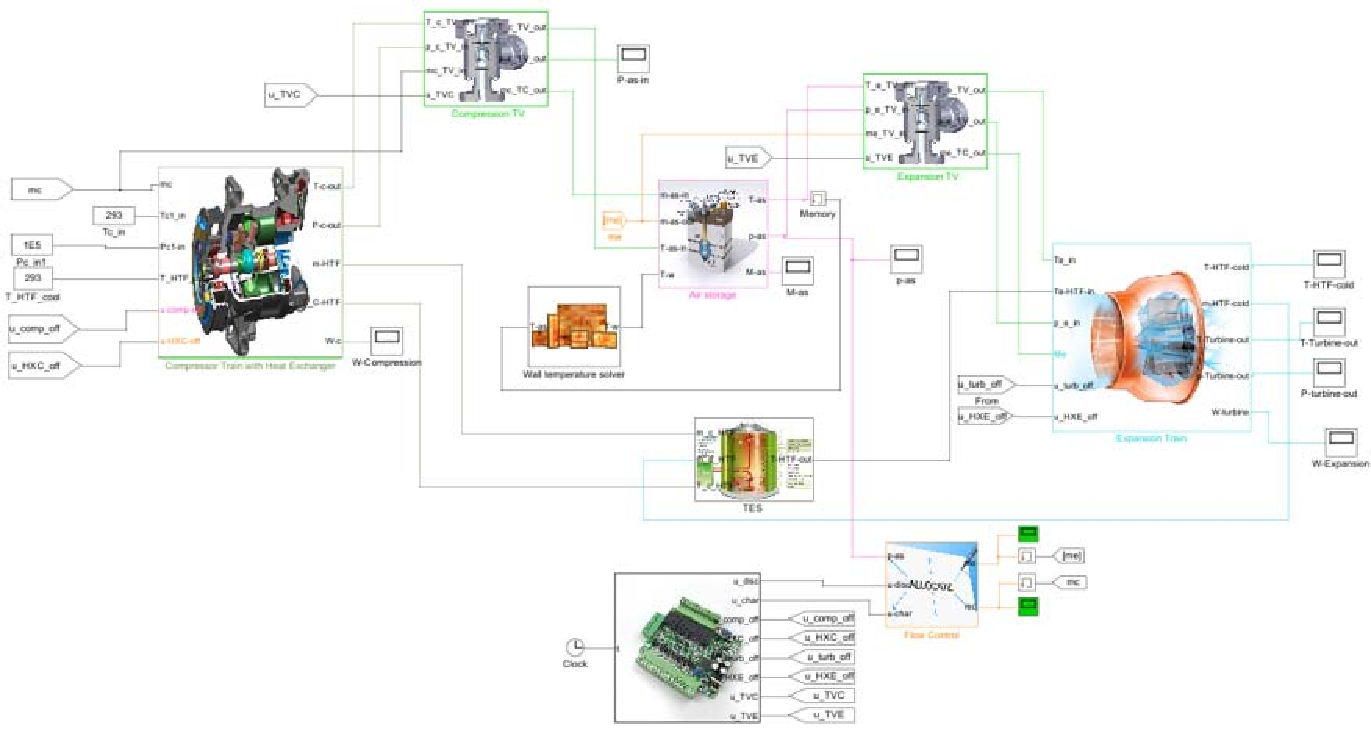
\includegraphics[scale=0.70]{Chap2-X-Simulation-Platform.pdf}
  \caption{计及组件部分负载特性的AA-CAES宽工况热力学仿真系统}
  \label{fig:Simulation-Platform}
\end{figure}

需要说明的是,目前存在可进行AA-CAES热力学特性仿真的软件,如Thermoflex 等,但其只能进行系统在任一给定运行点的性能,难以给出整个系统运行过程中的动态特性(储热系统、储气库),从而不便于分析一个循环周期内AA-CAES内部热力学参数间的相互耦合关系,同时也难以给出AA-CAES的宽工况运行特性。

\subsection{典型系统设计参数}
图\ref{fig:CAES-thermal-struc}给出了两级压缩两级膨胀的AA-CAES结构,尽管如此,本章的分析方法适用于任何多级压缩多级膨胀的AA-CAES系统的稳态热力学特性分析。本节基于所建的热力学稳态仿真模型分析一典型的小型AA-CAES系统的运行特性,该系统中的压缩机、膨胀机、换热器等组件的热力学设计参数分别见表
\ref{tab:TICC-500-para-comp} 至表\ref{tab:TICC-500-para-he-turb},相关数据基于文献~\inlinecite{Thesis-Wangsixian,Thesis-Zhangxuelin}改编而来。

我们假定采用文献\inlinecite{TICC-15}中的五级压缩三级膨胀结构,储气库无入口侧节流阀,但有出口侧节流阀,即AA-CAES运行于滑压-常压模式。同时,系统采用加压水作为HTF,相应的储热系统采用低温双罐储热结构。

%该系统参数常被用于AA-CAES相关研究的基准数据,如文献~\inlinecite{Variable-Conf-18,TICC-16}。

\begin{table}[htb]
  \centering
  \begin{minipage}[t]{0.79\linewidth} % 如果想在表格中使用脚注,minipage是个不错的办法
  \caption{压缩机额定参数}
  \label{tab:TICC-500-para-comp}
    \begin{tabularx}{\linewidth}{ccccccc}
      \toprule[1.5pt]
      {\heiti 级数} &  {\heiti $\beta_c$} & {\heiti $\eta_c$ (\%)} &  {\heiti $p_c^{in}$ (MPa)} & {\heiti $p_c^{out}$ (MPa)} & {\heiti $T_c^{in}$ ($^{\circ}$C)} & {\heiti $T_c^{out}$ ($^{\circ}$C)}\\
     \midrule[1pt]
      一级 & 3.5   & 74.4 & 0.1 & 0.35   & 25 & 153 \\
      二级 & 2.676 & 77.5 & 0.34 & 0.91  & 45 & 146.7 \\
      三级 & 2.697 & 80.5 & 0.89 & 2.40  & 45 & 147.6 \\
      四级 & 2.468 & 82.4 & 2.35 & 5.80  & 45 & 142.2 \\
      五级 & 1.963 & 83.0 & 5.72 & 11.23 & 45 & 109.1 \\
      \bottomrule[1.5pt]
    \end{tabularx}
  \end{minipage}
\end{table}

\begin{table}[htb]
  \centering
  \begin{minipage}[t]{0.79\linewidth} % 如果想在表格中使用脚注,minipage是个不错的办法
  \caption{膨胀机额定参数}
  \label{tab:TICC-500-para-turb}
    \begin{tabularx}{\linewidth}{ccccccc}
      \toprule[1.5pt]
      {\heiti 级数} & {\heiti $\beta_e$} &  {\heiti $\eta_e$ (\%)} & {\heiti $p_e^{in}$ (MPa)} & {\heiti $p_e^{out}$ (MPa)} & {\heiti $T_e^{in}$ ($^{\circ}$C)} &{\heiti $T_e^{out}$ ($^{\circ}$C)} \\
     \midrule[1pt]
      一级 & 2.212 & 82.6 & 2.50 & 1.13  & 100 & 12 \\
      二级 & 2.8 & 81.0 & 1.12 & 0.40  & 100 & 13 \\
      三级 & 3.714 & 81.6 & 0.39 & 0.105 & 100 & 13 \\
      \bottomrule[1.5pt]
    \end{tabularx}
  \end{minipage}
\end{table}

\begin{table}[htb]
  \centering
  \begin{minipage}[t]{0.88\linewidth} % 如果想在表格中使用脚注,minipage是个不错的办法
  \caption{压缩侧换热器额定参数}
  \label{tab:TICC-500-para-he-comp}
    \begin{tabularx}{\linewidth}{cccccc}
      \toprule[1.5pt]
      {\heiti 级数} & {\heiti $T_{c,HX}^{a,in}$ ($^{\circ}$C)} & {\heiti $T_{c,HX}^{a,out}$ ($^{\circ}$C)} & {\heiti $T_{c,HX}^{HTF,in}$ ($^{\circ}$C)} & {\heiti $T_{c,HX}^{HTF,out}$ ($^{\circ}$C)}&{\heiti $\dot m_{c,HX}^{HTF}$ (kg/s)}\\
     \midrule[1pt]
      一级 & 153   & 45 & 35 & 120  & 0.1346 \\
      二级 & 146.7 & 45 & 35 & 120  & 0.1268 \\
      三级 & 147.6 & 45 & 35 & 120  & 0.1279 \\
      四级 & 142.2 & 45 & 35 & 120  & 0.1212 \\
      五级 & 109.1 & 45 & 35 & 60   & 0.2755 \\
      \bottomrule[1.5pt]
    \end{tabularx}
  \end{minipage}
\end{table}

\begin{table}[htb]
  \centering
  \begin{minipage}[t]{0.89\linewidth} % 如果想在表格中使用脚注,minipage是个不错的办法
  \caption{膨胀侧换热器额定参数}
  \label{tab:TICC-500-para-he-turb}
    \begin{tabularx}{\linewidth}{cccccc}
      \toprule[1.5pt]
      {\heiti 级数} & {\heiti $T_{e,HX}^{a,in}$ ($^{\circ}$C)} & {\heiti $T_{e,HX}^{a,out}$ ($^{\circ}$C)} & {\heiti $T_{e,HX}^{HTF,in}$ ($^{\circ}$C)} & {\heiti $T_{e,HX}^{HTF,out}$ ($^{\circ}$C)} & {\heiti $\dot m_{e,HX}^{HTF}$ (kg/s)}\\
     \midrule[1pt]
      一级 & -15 & 100 & 120 & 35  & 0.7855\\
      二级 & 30  & 100 & 120 & 35  & 0.5936\\
      三级 & 25  & 100 & 120 & 35  & 0.5943\\
      \bottomrule[1.5pt]
    \end{tabularx}
  \end{minipage}
\end{table}

\subsection{设计工况性能}
\label{sec:chap2-model-valid-Thermoflex}
额定设计点的运行性能分析旨在说明AA-CAES内部各组件运行特性之间的相互影响,我们重点分析AA-CAES在滑压-常压运行模式下能量转换类组件(压缩机、膨胀机)及能量转移类组件(换热器)的运行特性与能量存储类组件(储气库及储热罐)的动态特性之间的耦合关系。

\subsubsection{压缩储能过程}
我们设定储气库的运行压力范围为4MPa-10MPa,储气库的体积取为100 m$^2$(与文献\inlinecite{TICC-15}中的实际电站一致)。压缩储能过程以压缩机的额定质量流率(0.4492kg/s)进行压缩储能,在给定的压缩侧滑压运行模式下,压缩储能过程的总时间为2.9h,各级压缩机的出口空气压力的变化过程如图
\ref{fig:Sim-Char-Inlet-Pressure}所示。

\begin{figure}[H] % use float package if you want it here
  \centering
  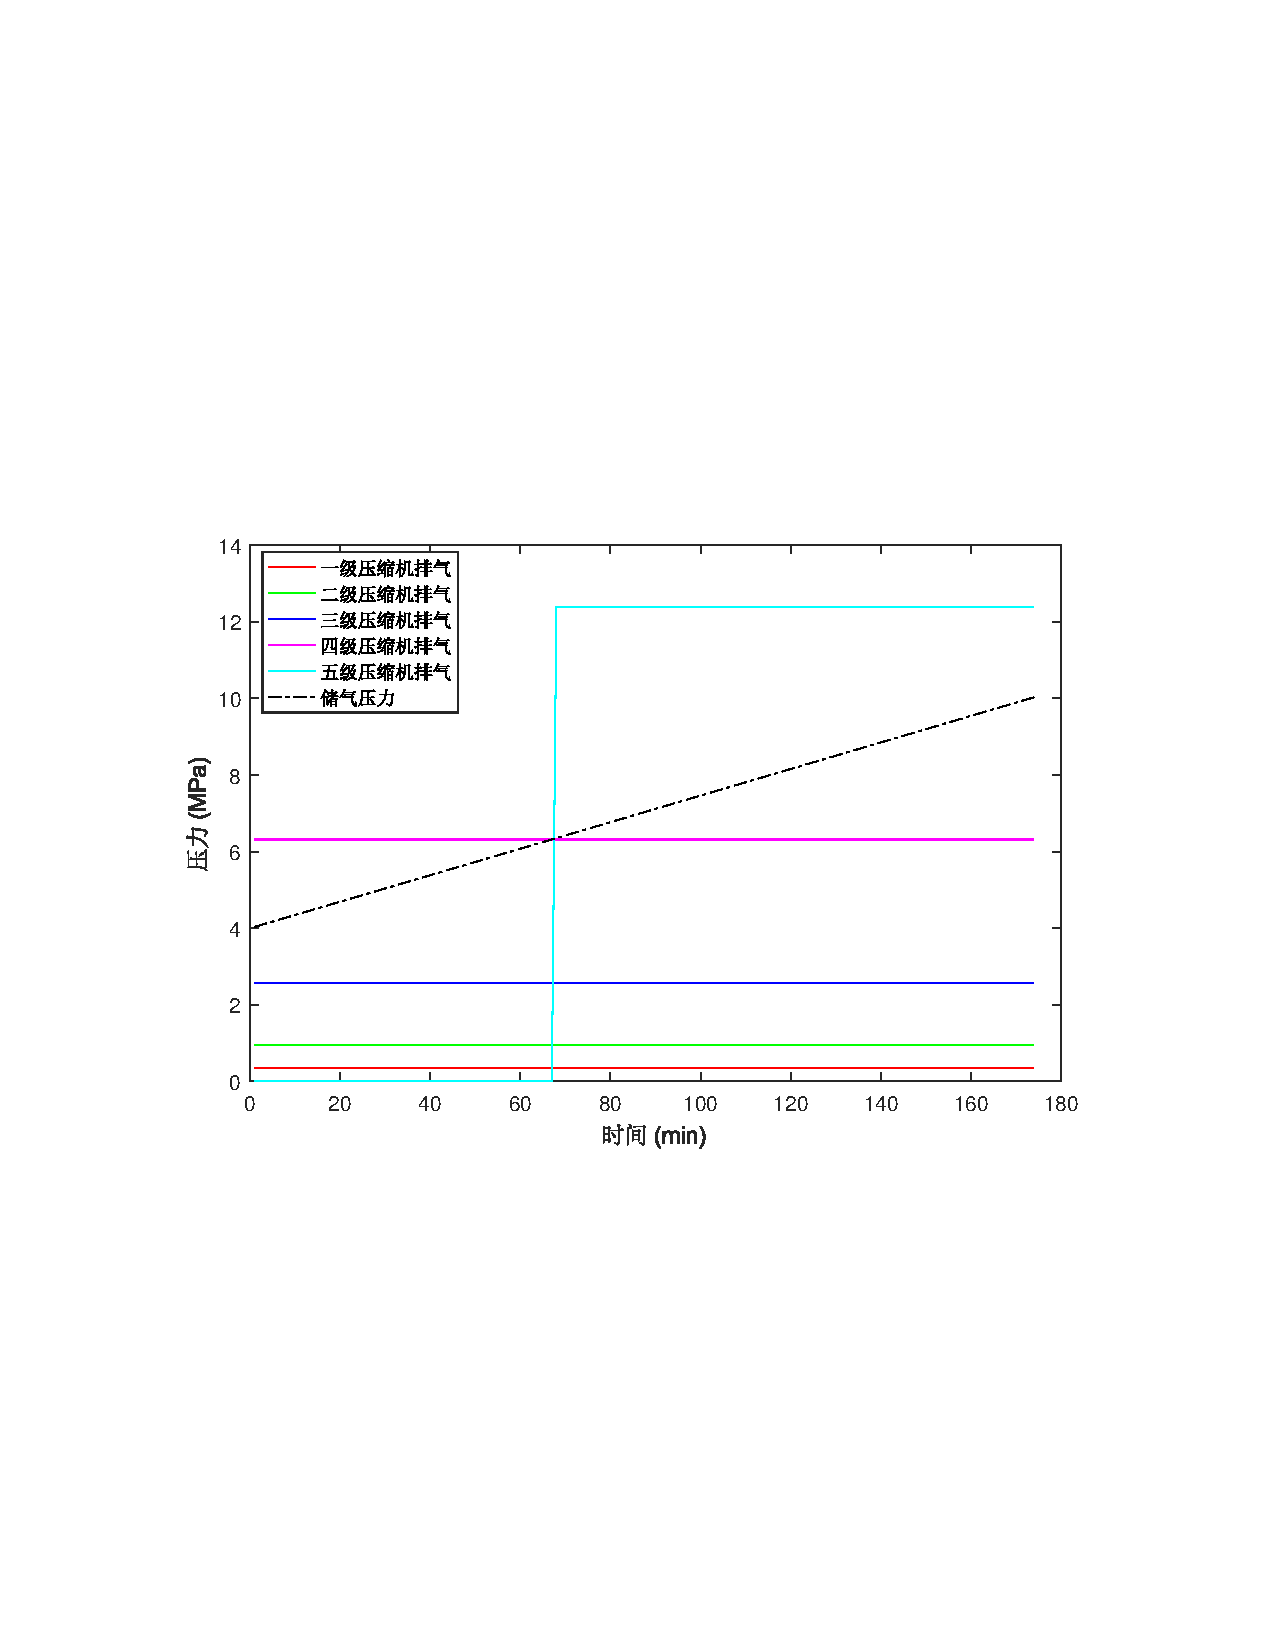
\includegraphics[scale=0.70]{Chap2-Sim-Char-Inlet-Pressure.pdf}
  \caption{压缩储能过程各级压缩机出口压力变化曲线(设计工况)}
  \label{fig:Sim-Char-Inlet-Pressure}
\end{figure}

由于压缩侧采用了滑压运行模式,压缩机将承受储气库背压,而随着储能过程的进行,储气库压力升高,压缩机承受的背压也将增大,各级压缩机的运行状态也有所不同。压缩初始状态,储气库压力为4MPa,需要启动前四级压缩机;随着储气库空气压力增至6.2MPa(第65min),第5级压缩机启动,从而将末级压缩机的出口空气压力提升至10MPa以上,以克服储气库的实时压力进行储气。此外,由于我们设定不考虑换热器的压损特性,导致每级压缩机的排气压力略高于额定排气压力。

对于小型AA-CAES,由于储气库体积较小,容易实现绝热储气,我们采用了VA模型。在储能过程中储气库中空气的热力学动态如图\ref{fig:Sim-Char-ASU-P-M}所示。在VA模型的设定下,储气库不与外界进行换热,随着高压空气(高温)的注入,储气库内空气的质量、温度及压力均上升。为了维持储气库的最低运行压力,储气库在初始状态需存储一定的空气,由理想气体状态方程可得初始空气质量为4.7617$\times10^3$ kg/,由于以额定质量流率储气,储气库中空气质量线性增长。

\begin{figure}[H] % use float package if you want it here
  \centering
  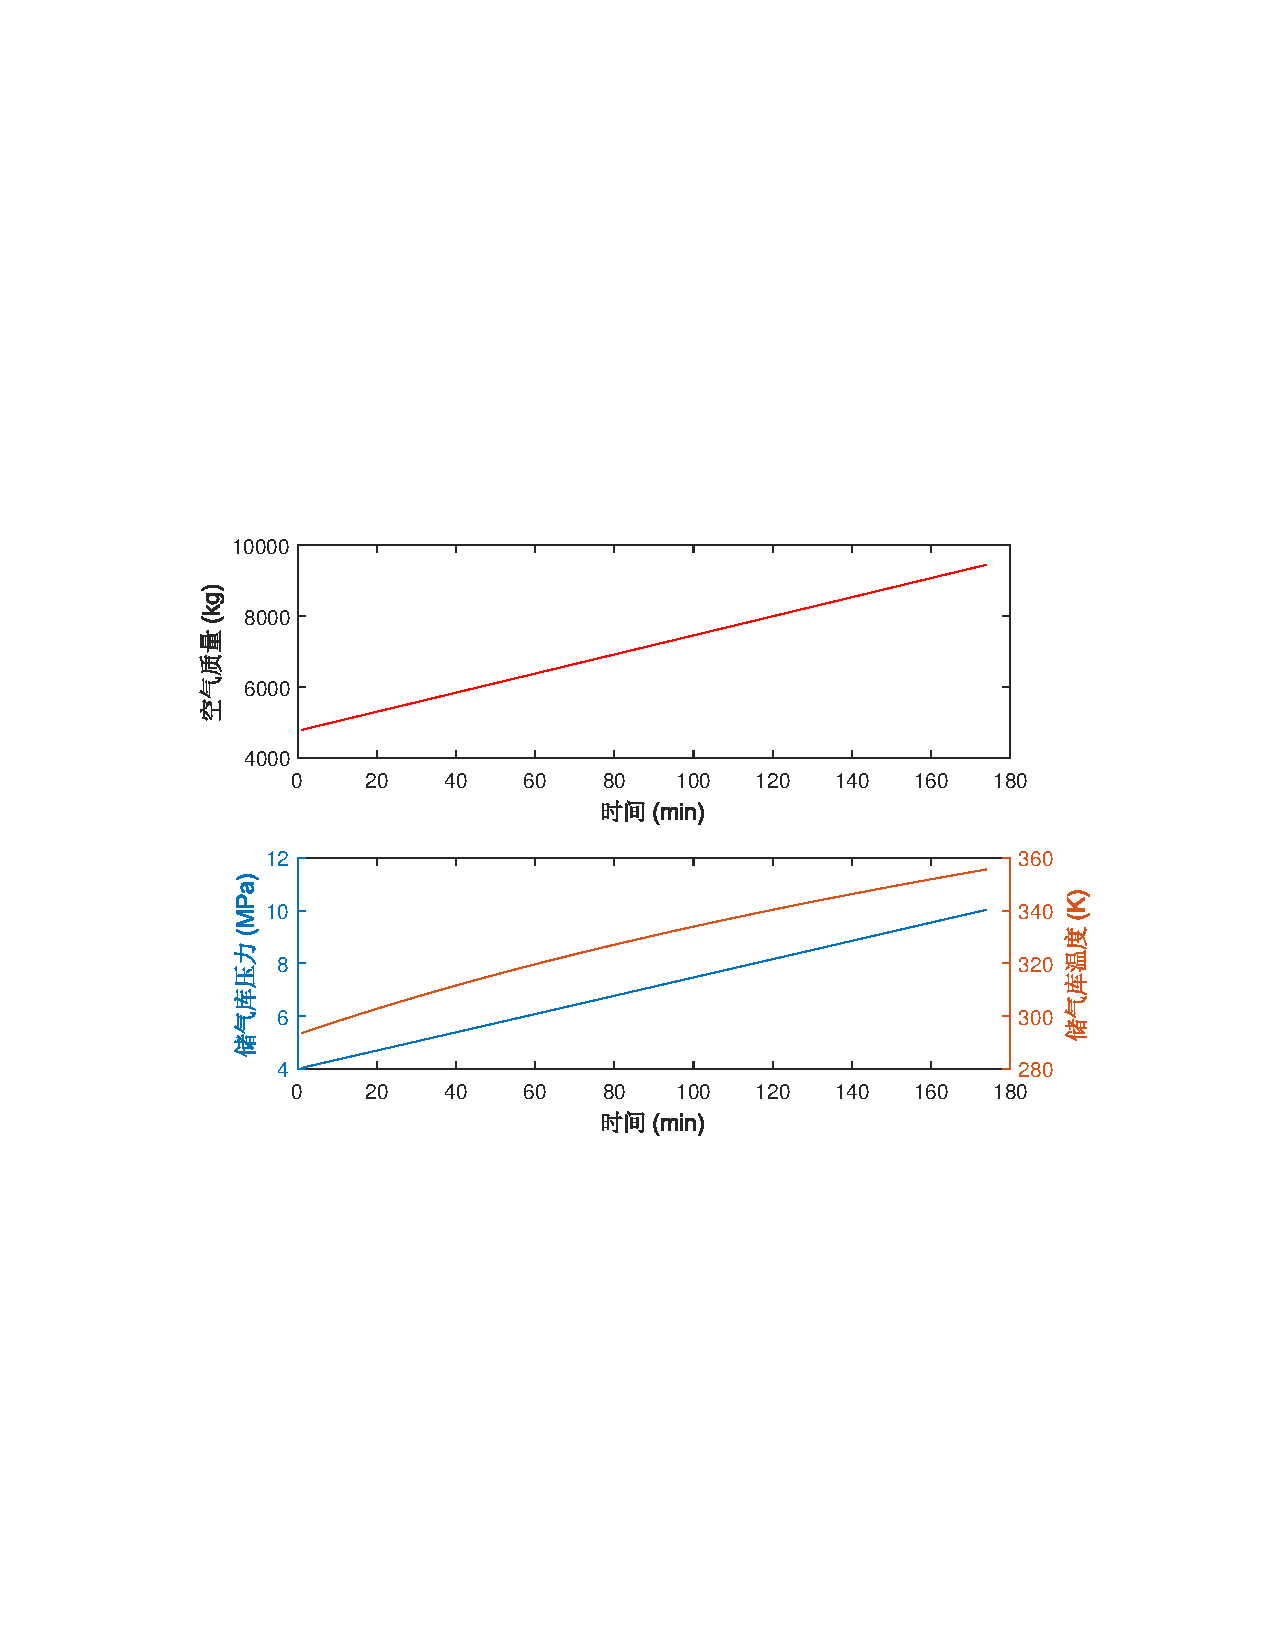
\includegraphics[scale=0.75]{Chap2-Sim-Char-ASU-P-M.pdf}
  \caption{压缩储能过程储气库动态特性(设计工况)}
  \label{fig:Sim-Char-ASU-P-M}
\end{figure}

在第5级压缩机未启动前,储气库进口空气的热力学参数由第4级换热器出口空气决定,当第5级压缩机启动后则由第5级换热器出口空气的热力学参数决定。因此,储气库的压力呈现两段线性增长趋势,而温度与储气库中空气的实时质量有关,并不线性增长。

\begin{figure}[H] % use float package if you want it here
  \centering
  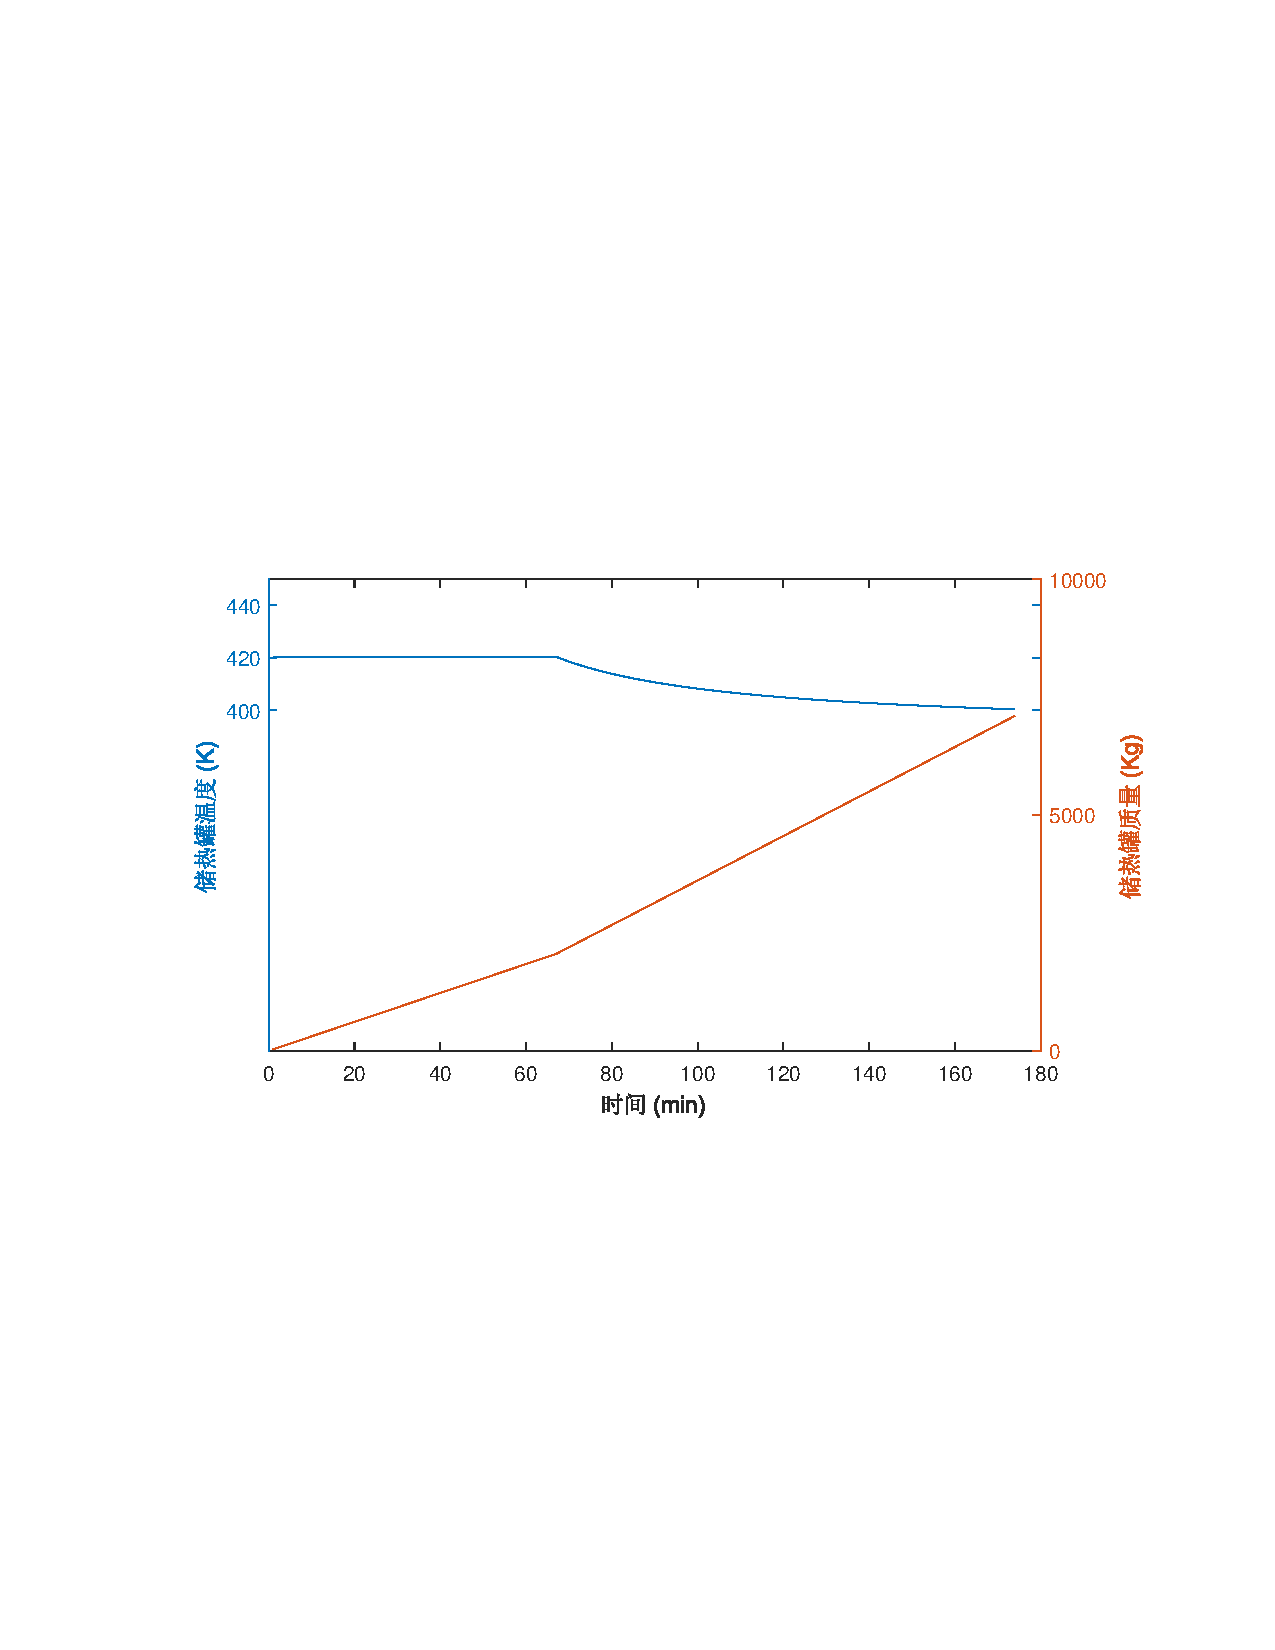
\includegraphics[scale=0.70]{Chap2-Sim-Char-TES.pdf}
  \caption{压缩储能过程储热罐动态特性(设计工况)}
  \label{fig:Sim-Char-TES}
\end{figure}

小容量储热系统容易实现绝热模型,我们假定系统在储能初始状态下高温储热罐中HTF的质量为0,压缩储能过程中高温储热罐的HTF的热力学动态特性如图
\ref{fig:Sim-Char-TES}所示。在第5级压缩机未启动之前,由于以额定质量流率压缩,HTF侧也以固定的质量流率进行储热(一般维持换热器的热容比$C_{c,HX}$为定值),储热罐中的HTF质量增大。第5级压缩机启动后,注入储热罐中的HTF质量流率将进一步增大,从而增大了储热罐中HTF 质量变化的斜率。同时,由于前五级换热器的HTF汇合温度(392.12K)低于前四级换热器的HTF汇合温度(420.30K),导致储热罐中HTF的温度从第56min起先下降(根据温度混合方程),随着储热过程的结束,HTF的温度渐渐平稳。储热过程结束时,储热罐中的HTF总质量为7.0973$\times 10^3$ kg,HTF的温度为400.27K。

在设计工况下,压缩侧各级换热器的换热功率及各级压缩机的耗功变化曲线分别如图\ref{fig:Sim-Char-Heat-Quan}及图\ref{fig:Sim-Char-Comp-Power}所示。由于我们假定AA-CAES 内部各组件在设计质量流率下以额定等熵效率运行,因此各级换热器的换热器量均为设计值,换热器运行于额定等熵效率。尽管各级换热器的HTF侧进口温度均为308.15K,但由于各级的热容比以及入口空气温度的差异,其换热功率不同。
\begin{figure}[H] % use float package if you want it here
  \centering
  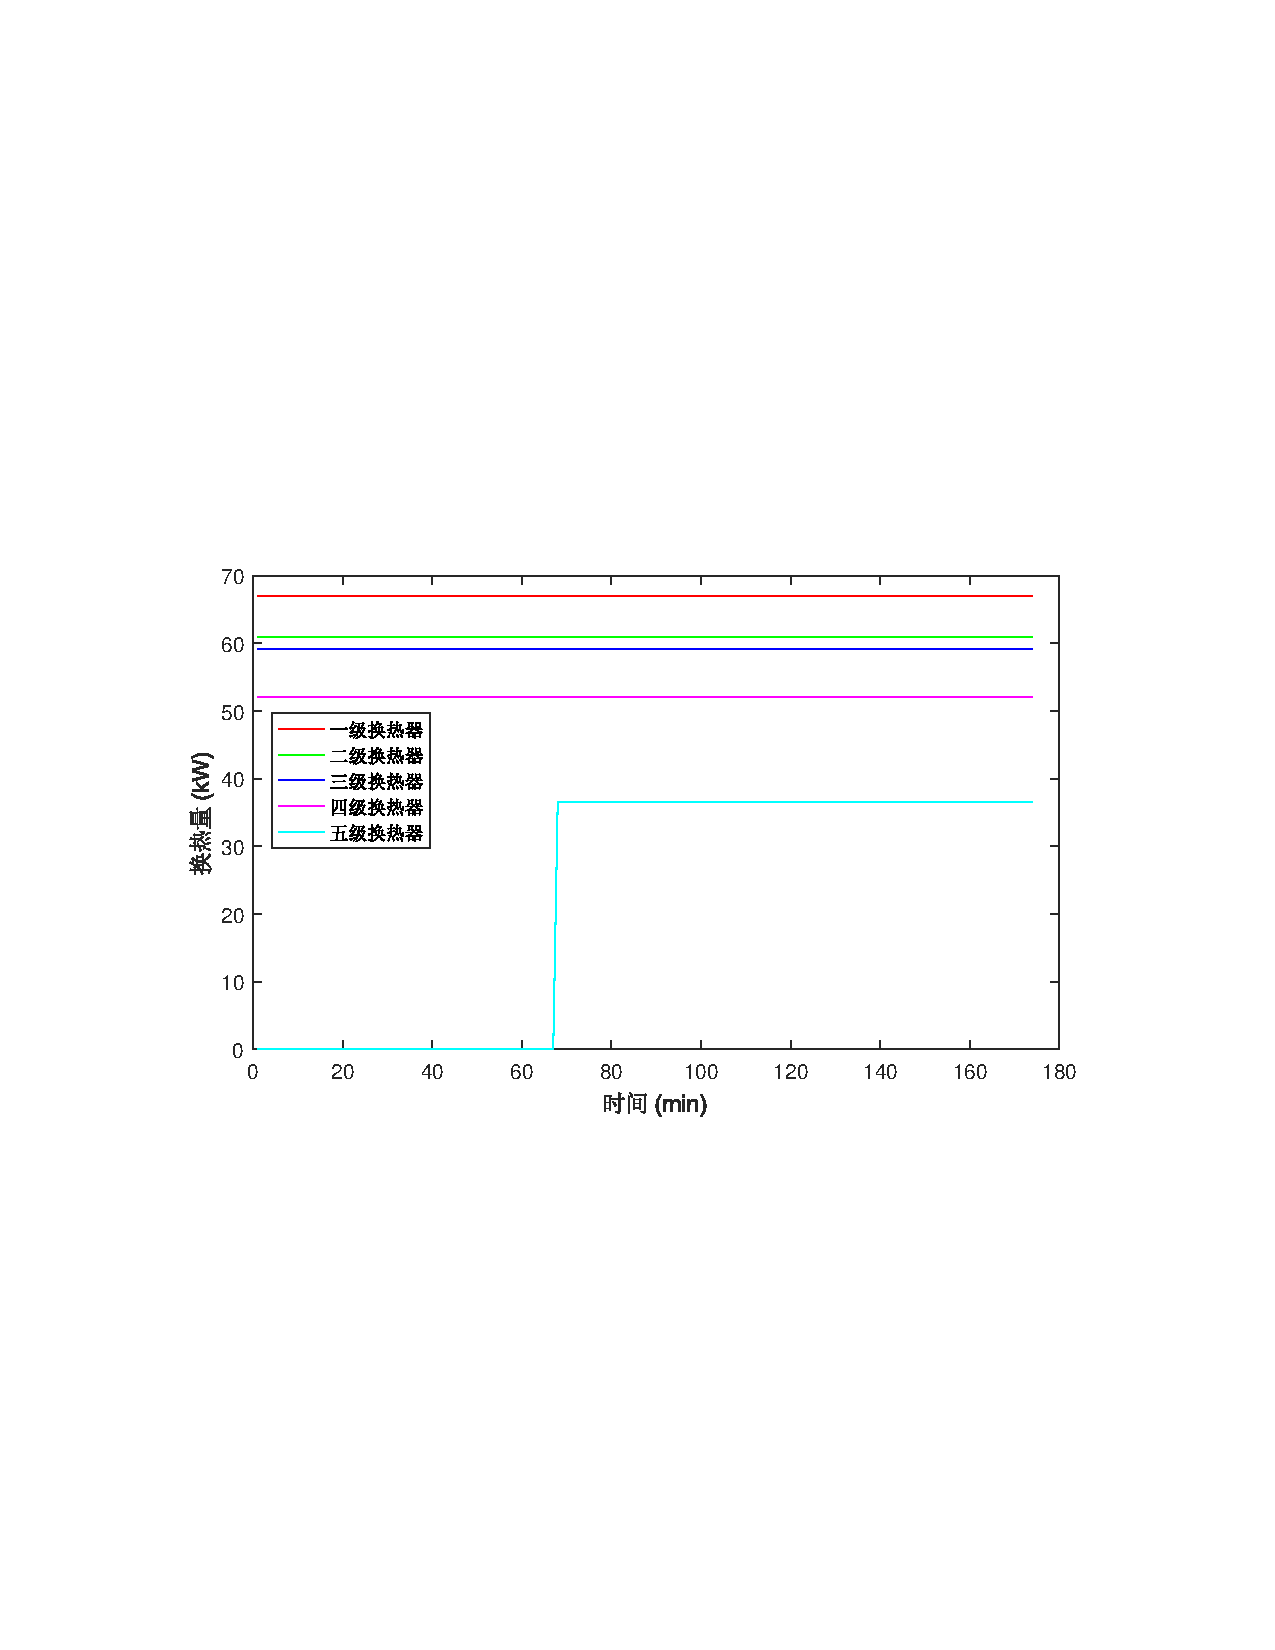
\includegraphics[scale=0.66]{Chap2-Sim-Char-Heat-Quan.pdf}
  \caption{压缩储能过程换热器换热功率变化曲线(设计工况)}
  \label{fig:Sim-Char-Heat-Quan}
\end{figure}

同时,在第5级压缩机未启动前,第1级至第4级压缩机消耗的额定电功率分别为77.73 kW,60.79 kW,58.98 kW,51.69 kW,系统总耗功为249.21kW;第5级压缩机启动后并消耗电功率36.93kW,从而将储能过程消耗的电功率提升至286.14kW。因此,我们不难发现,在压缩侧的滑压运行模式下,整个压缩储能过程不能一直实现满压缩功率储能,但各级压缩机可运行在额定设计工况。

\begin{figure}[H] % use float package if you want it here
  \centering
  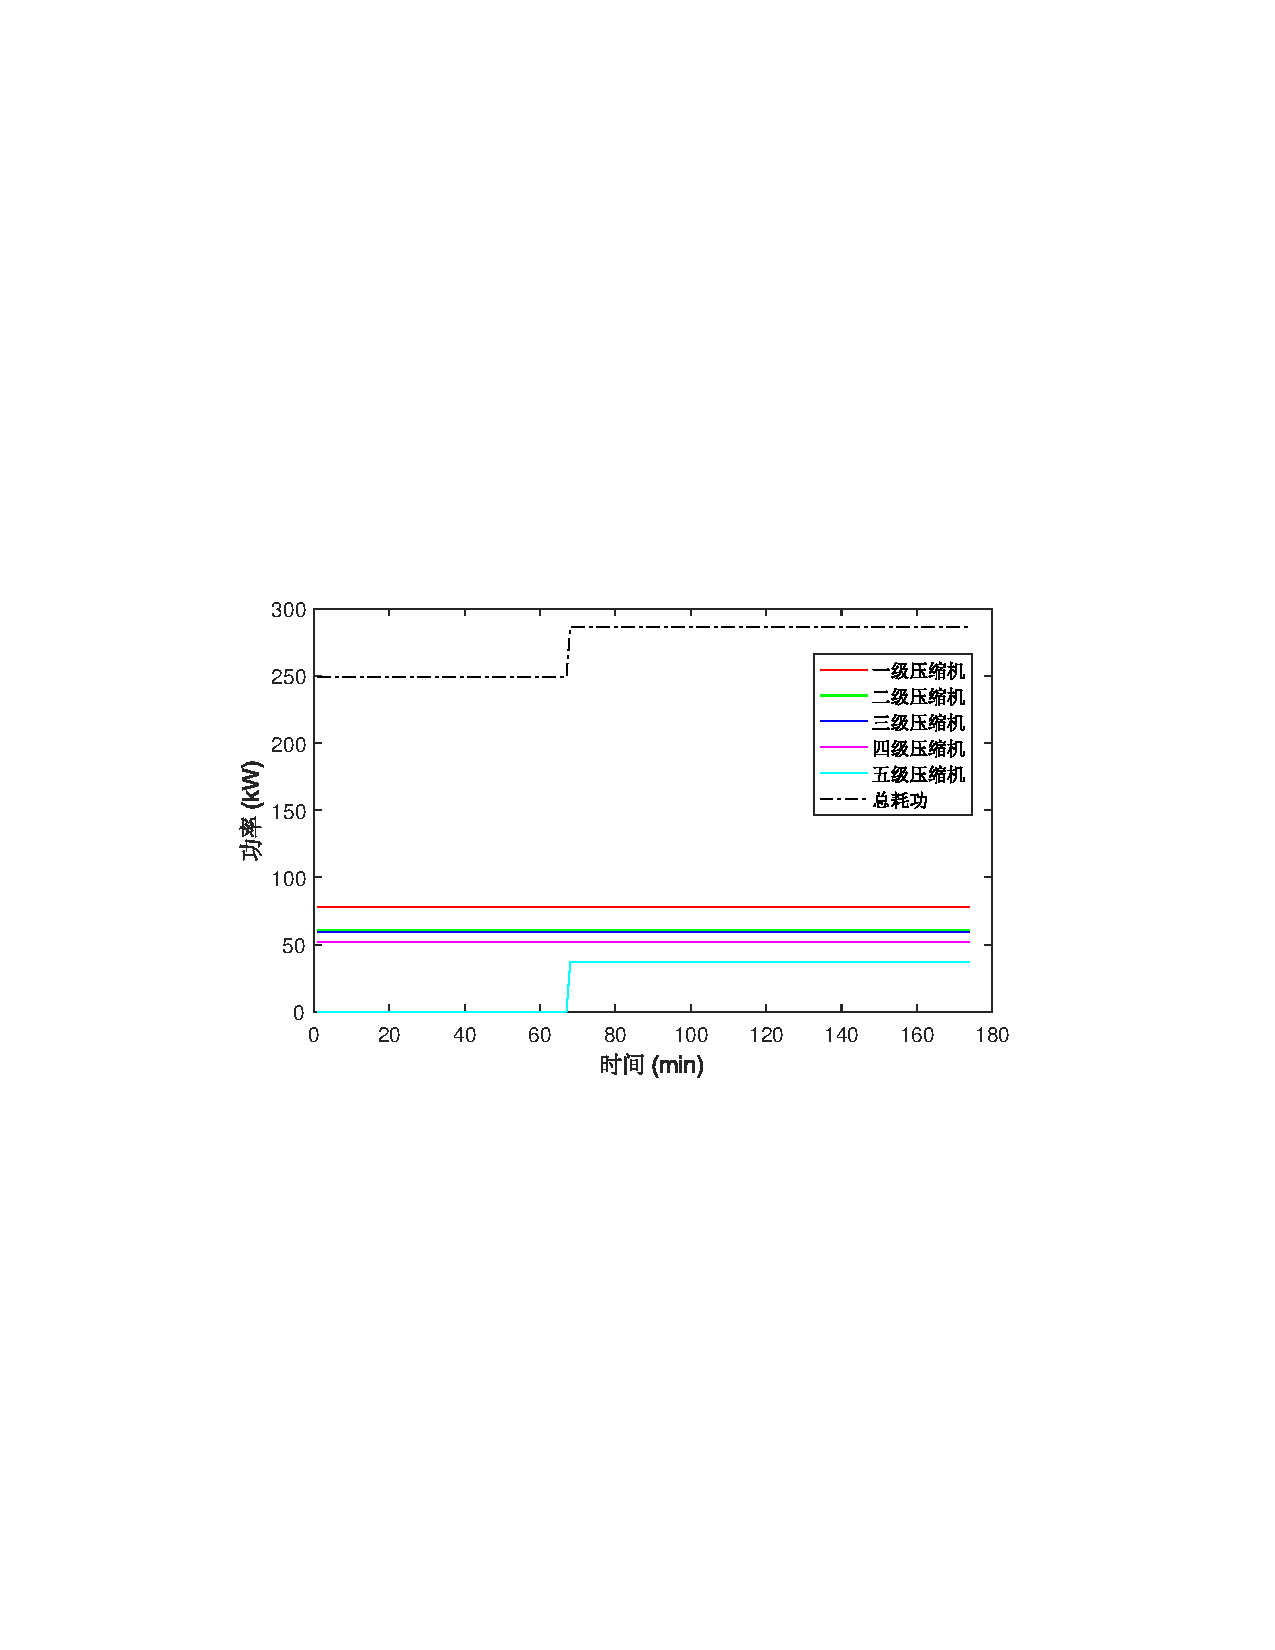
\includegraphics[scale=0.76]{Chap2-Sim-Char-Comp-Power.pdf}
  \caption{压缩储能过程压缩机耗功变化曲线(设计工况)}
  \label{fig:Sim-Char-Comp-Power}
\end{figure}
%需要说明的是,就整个AA-CAES对外特性而言,压缩侧处于滑压运行模式时

\subsubsection{膨胀释能过程}
与压缩储能过程类似,我们以膨胀机的额定质量流率(2.4435kg/s)进行膨胀释能,在给定的膨胀侧常压运行模式下,储气库的热力学动态特性如图
\ref{fig:Sim-Disc-ASU-P-T-M}所示,总释能时间为0.53h。由于采用了常压运行模式,第1级透平的进气压力为储气库的最低运行压力,即4MPa,随着释能过程的进行,储气库中空气的压力逐渐从压缩储能末端时的储气压力10MPa 逐渐减小,当储气压力减至储气库的最低运行压力时,释能过程结束。储气库内空气质量线性减少,而压力与温度并不呈线性趋势,其原因在于储气压力不仅与质量流率有关,还与储气库内空气的温度有关,而空气温度与时变的储气库空气质量有关。

\begin{figure}[H] % use float package if you want it here
  \centering
  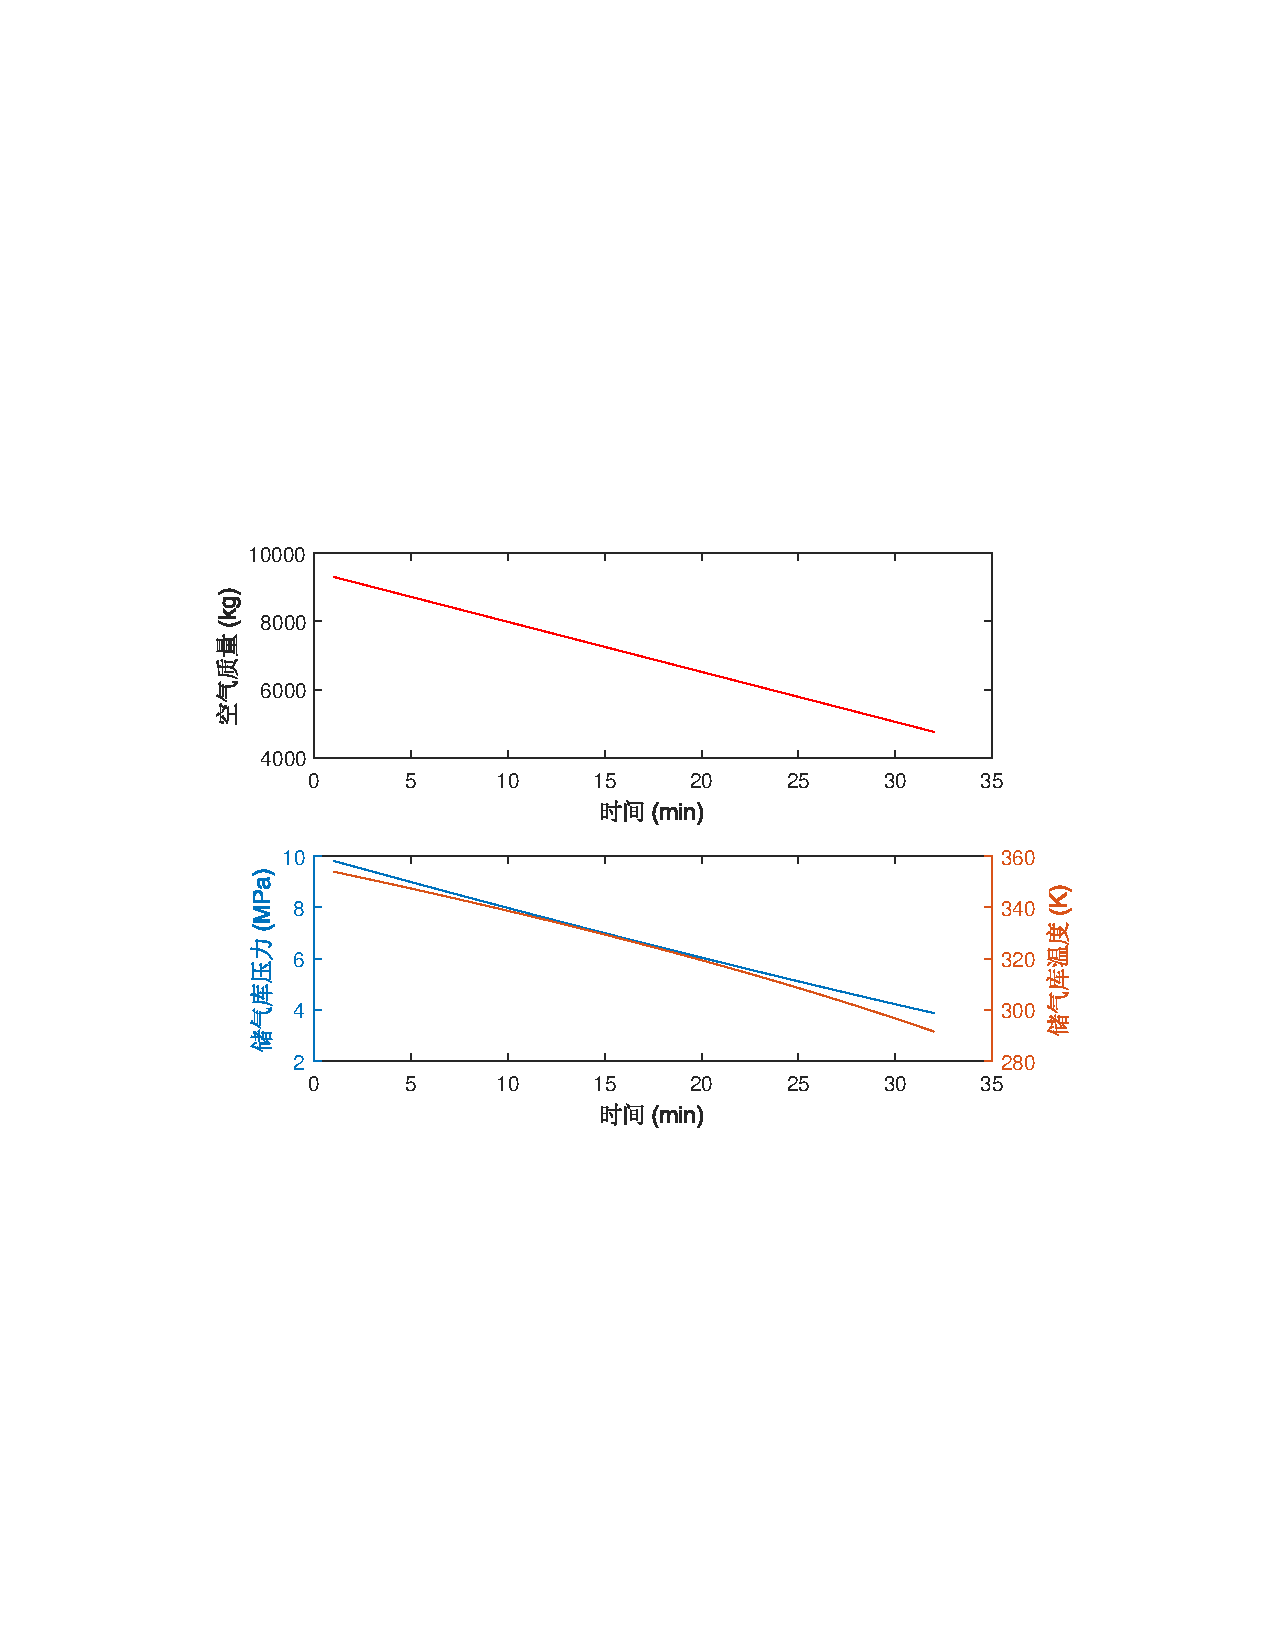
\includegraphics[scale=0.74]{Chap2-Sim-Disc-ASU-P-T-M.pdf}
  \caption{膨胀释能过程储气库动态特性(设计工况)}
  \label{fig:Sim-Disc-ASU-P-T-M}
\end{figure}

在储气库VA模型下,随着储气库中空气质量的减少,储气库中空气温度也持续下降,从释能开始时的355.58 K降至释能结束时的291.47K,进而逐渐增大了对
膨胀释能阶段各级换热器的换热功率需求。由图\ref{fig:Sim-Disc-Heat-Quan}所示的换热器换热功率变化曲线可以看出,1级换热器换热功率需求的变化最明显,从膨胀释能初始时的93.35kW,逐渐增至释能终止时的221.9kW,变化幅度达137.71\%;2级换热器换热功率的变化范围较小,从释能开始时的138.49kW增至释能结束时的152.94kW,增幅为10.43\%;3级换热器的换热功率基本维持不变。由此可以得出,随着释能过程的进行,越靠近储气库的换热器换热功率的变化越大,而后级换热器换热功率的变化越来越小,其主要原因在于通过前级换热器的“缓冲”,后级换热器的进口空气温度在释能过程中可以维持在较小的变化范围。

\begin{figure}[H] % use float package if you want it here
  \centering
  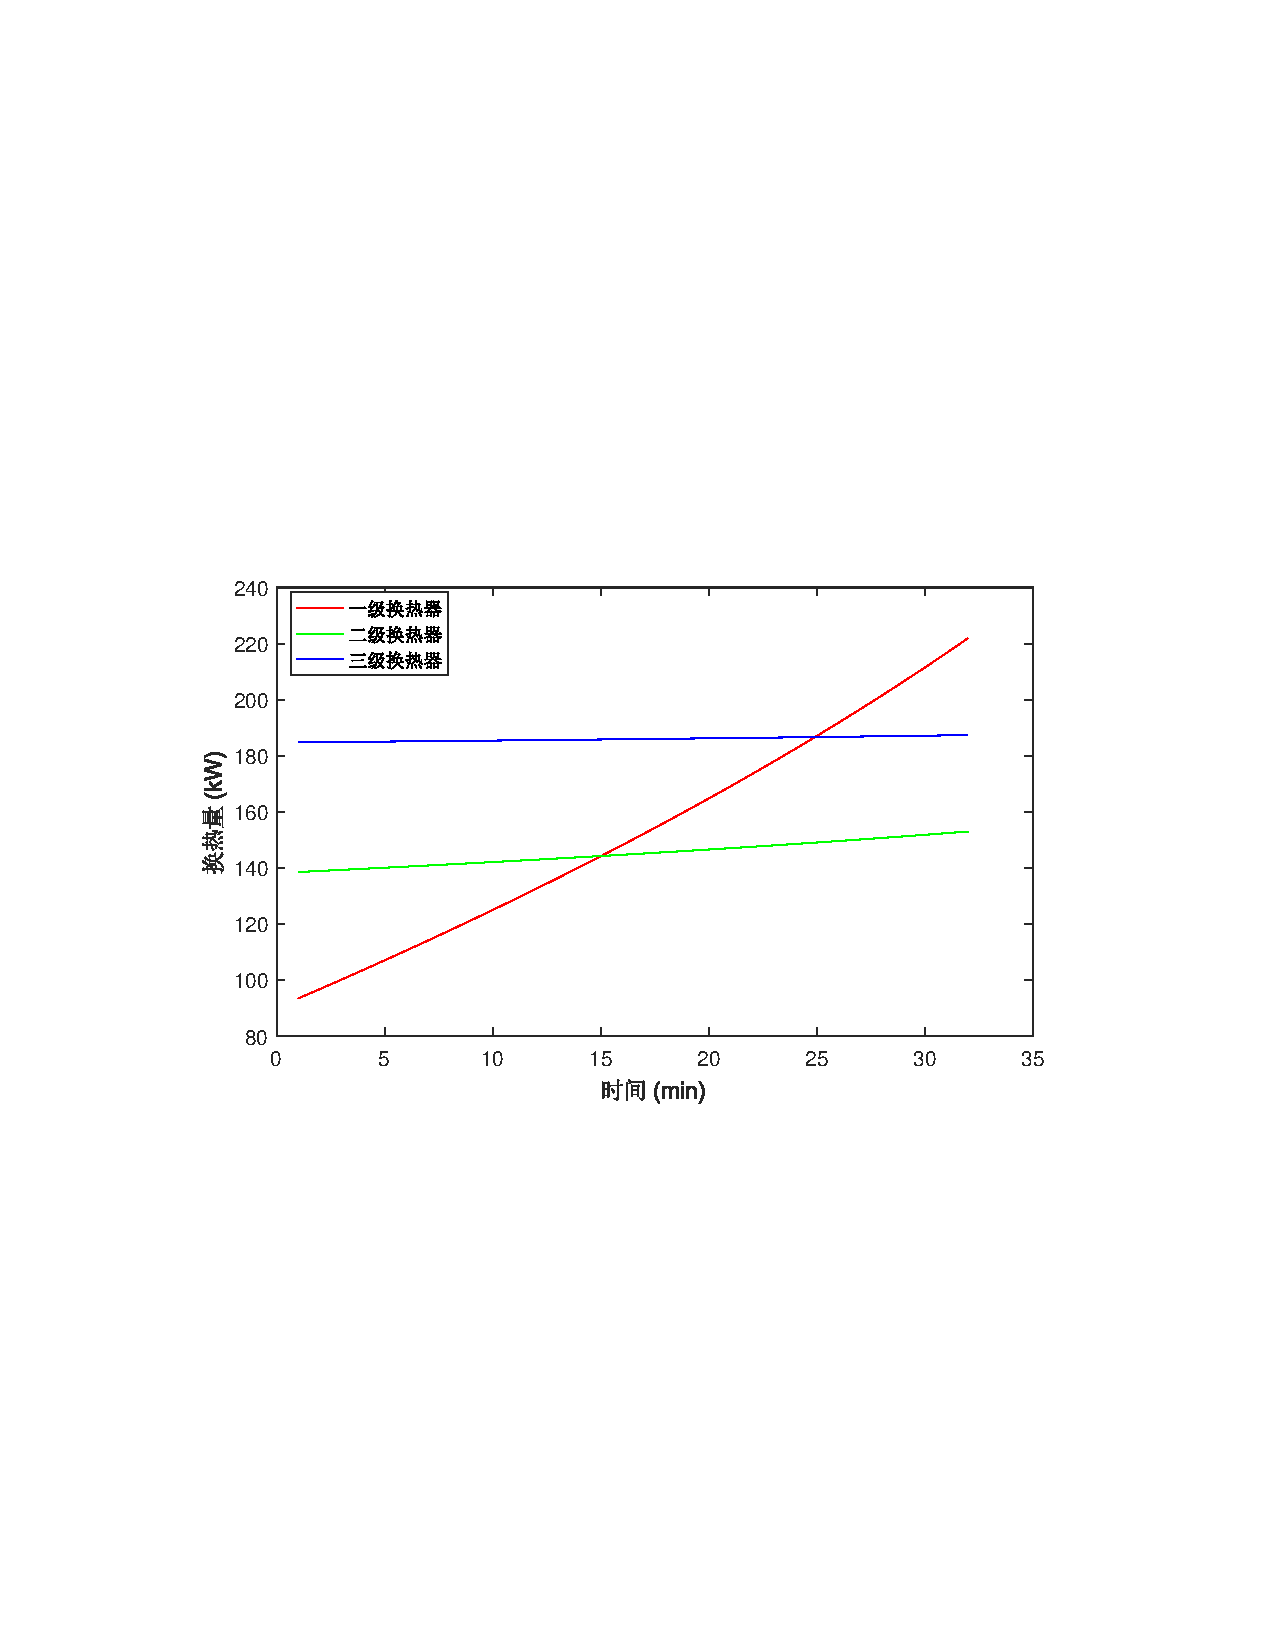
\includegraphics[scale=0.75]{Chap2-Sim-Disc-Heat-Quan.pdf}
  \caption{膨胀释能过程换热器换热功率(设计工况)}
  \label{fig:Sim-Disc-Heat-Quan}
\end{figure}

与图\ref{fig:Sim-Disc-Heat-Quan}中换热器换热功率的变化一致,随着释能过程中储气库内空气压力及温度的降低,各级透平的输出功率也相应下降,但变化不大。图
\ref{fig:Sim-Disc-Turb-Power}给出了膨胀释能过程中第1级透平输出功率及AA-CAES系统的总膨胀功率的变化曲线。第1级透平的输出功率从161.8kW减至158.06kW,变化率为2.31\%,三级透平的总输出(电)功率从594.06kW减至589.29kW,变化仅为0.8\%。由此可见,通过换热器及储热系统的配合,让换热器承担(或缓解)储气库内空气温度的下降对释能过程的影响,即可在透平侧的定压运行模式下实现稳定的功率输出,可以说,这正是AA-CAES这一储能循环采用储气与储热实现“气热双储”带来的灵活性。

\begin{figure}[H] % use float package if you want it here
  \centering
  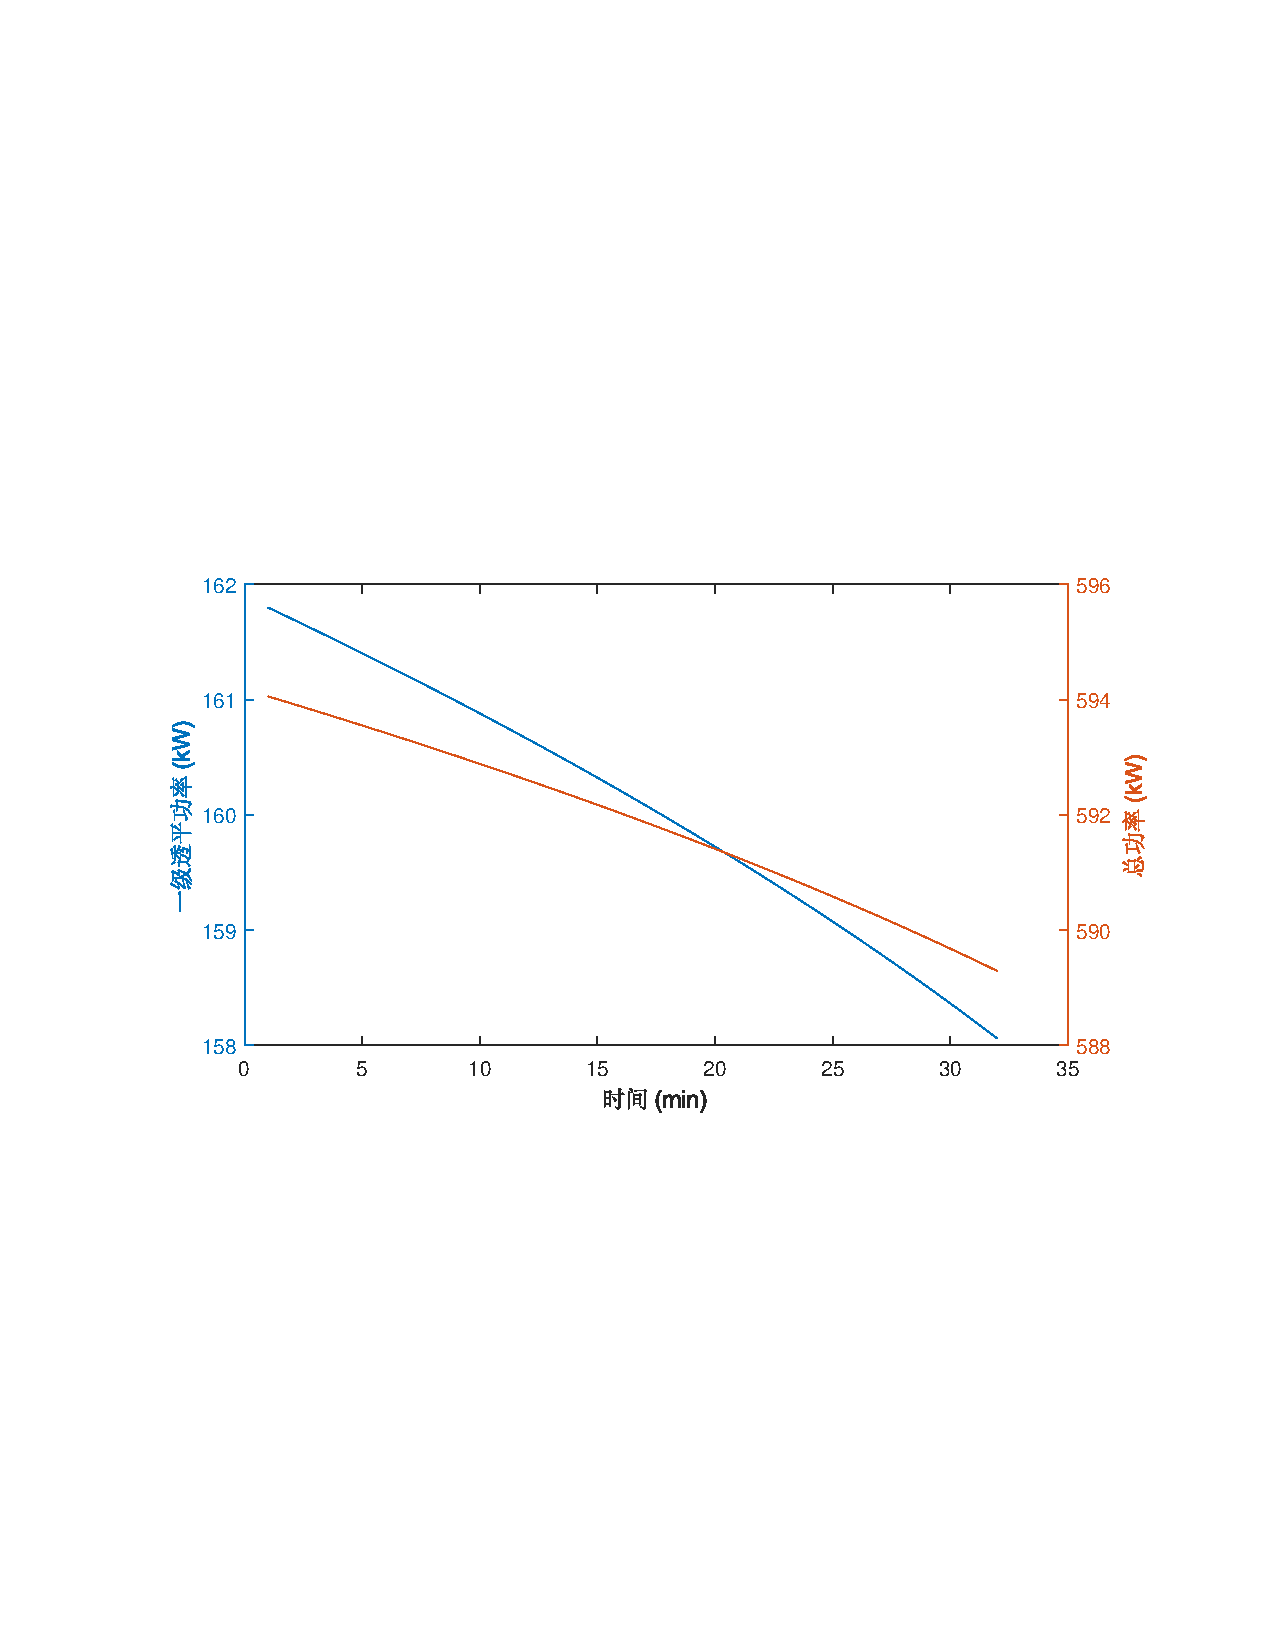
\includegraphics[scale=0.72]{Chap2-Sim-Disc-Turb-Power.pdf}
  \caption{膨胀释能过程输出功率变化曲线(设计工况)}
  \label{fig:Sim-Disc-Turb-Power}
\end{figure}

综上,在滑压-定压运行模式下,以额定质量流率进行储能与释能的一个循环周期中,AA-CAES消耗的总电量为0.7886MWh,输出的总电量为0.3157MWh,其电-电效率$\eta_{elec}$为40.03\%。 同时,储能结束时高温储热罐中的HTF质量为6.9784$\times 10^3$kg,释能结束时储热罐中剩余的高温HTF质量为3.2941$\times10^3$kg,温度为400.27K,该部分热水可用于供热,总供热量可达0.3524MWh,供热效率$\eta_{heat}$为44.69\%,系统热电联供的总能利用系数$\eta_{total}$为84.72\%。供热量的热量㶲为0.0944MWh,供热㶲效率$\eta_{x,heat}$为11.97\%,热电联供总㶲效率$\eta_{x,total}$为52\%。此外,尽管本文不关注制冷,但透平末级排气温度(283.01K)低于环境温度,该部分能量可用于制冷,进而AA-CAES多能联供的总能利用系数及㶲效率均可提高。事实上,图\ref{fig:Sim-Char-Inlet-Pressure}中第5级压缩机排气压力高于储气库的实时压力,存在一定的能量损失,若让第5级压缩机运行于一定的非设计工况,使得其排气压力与储气库压力一致,即可降低第5级压缩机的耗功,从而可进一步提升系统的各能效指标。

\subsection{部分负载性能}
\label{sec:chap2-model-valid-TICC}
实际运行过程中,除了内部组件之间的耦合关系之外,能量转换类组件(压缩机、膨胀机)及能量转移类组件(换热器)的部分负载运行特性对AA-CAES系统运行特性也有着重要的影响。特别是,当挖掘AA-CAES的容量备用等灵活性特性时,压缩储能过程中的质量流率与膨胀释能过程中的质量流率将偏离压缩机与膨胀机(及与之匹配的换热器)的额定质量流率,进而影响内部能量转换、能量转移及能量存储组件的热力学特性。我们以图\ref{fig:Sim-massflow-Part-load}所示的部分负载质量流率模拟电力系统对AA-CAES的宽工况运行要求,进而分析对应的压缩储能与膨胀释能过程。

\begin{figure}[H] % use float package if you want it here
  \centering
  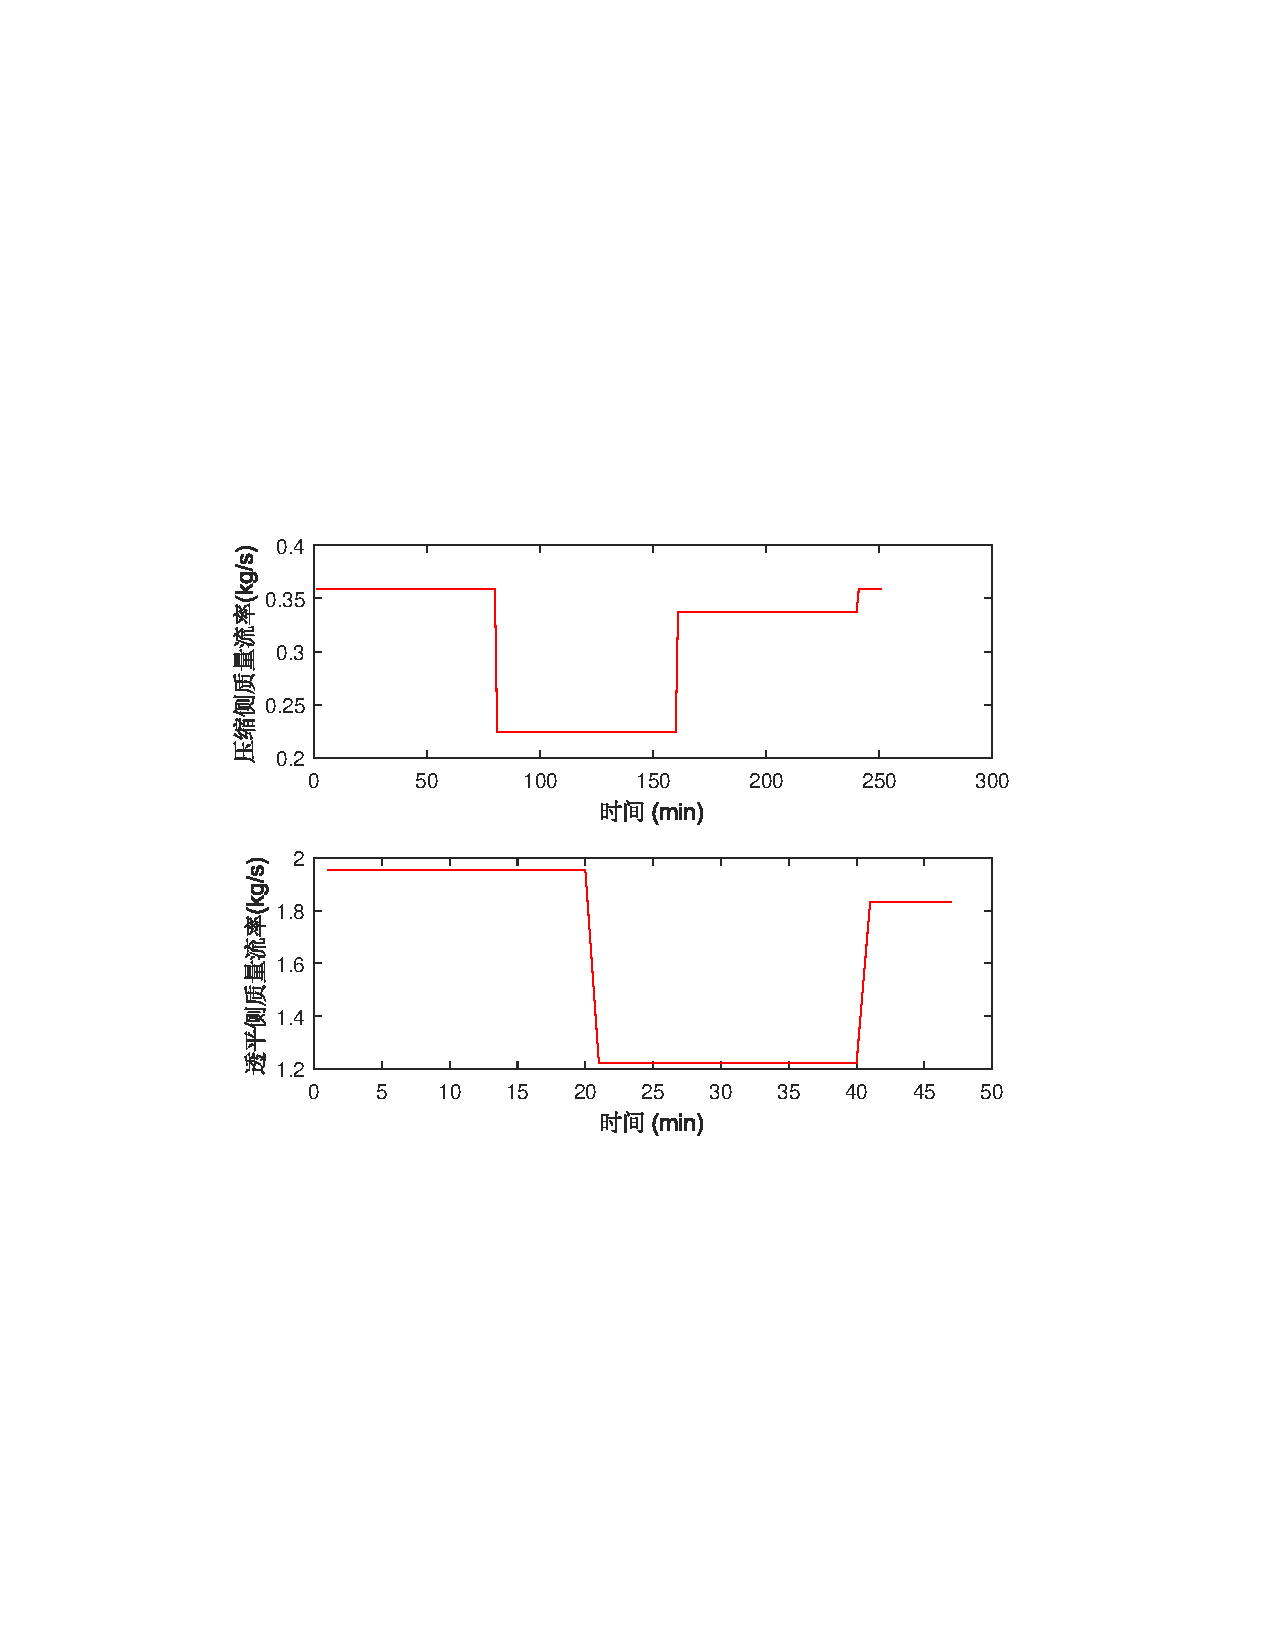
\includegraphics[scale=0.75]{Chap2-Sim-massflow-Part-load.pdf}
  \caption{模拟部分负载模式的质量流率曲线}
  \label{fig:Sim-massflow-Part-load}
\end{figure}

\subsubsection{压缩储能过程}
在压缩侧滑压运行模式下,按照图\ref{fig:Sim-massflow-Part-load}所示的质量流率进行压缩储能的过程中,压缩侧的质量流率的减小导致整个储能运行时间由设计工况下的2.9h 增长为4.18h。图\ref{fig:Sim-Char-Inlet-Pressure-Part-load}给出了部分负载运行模式下各级压缩机入口压力的变化曲线。

\begin{figure}[H] % use float package if you want it here
  \centering
  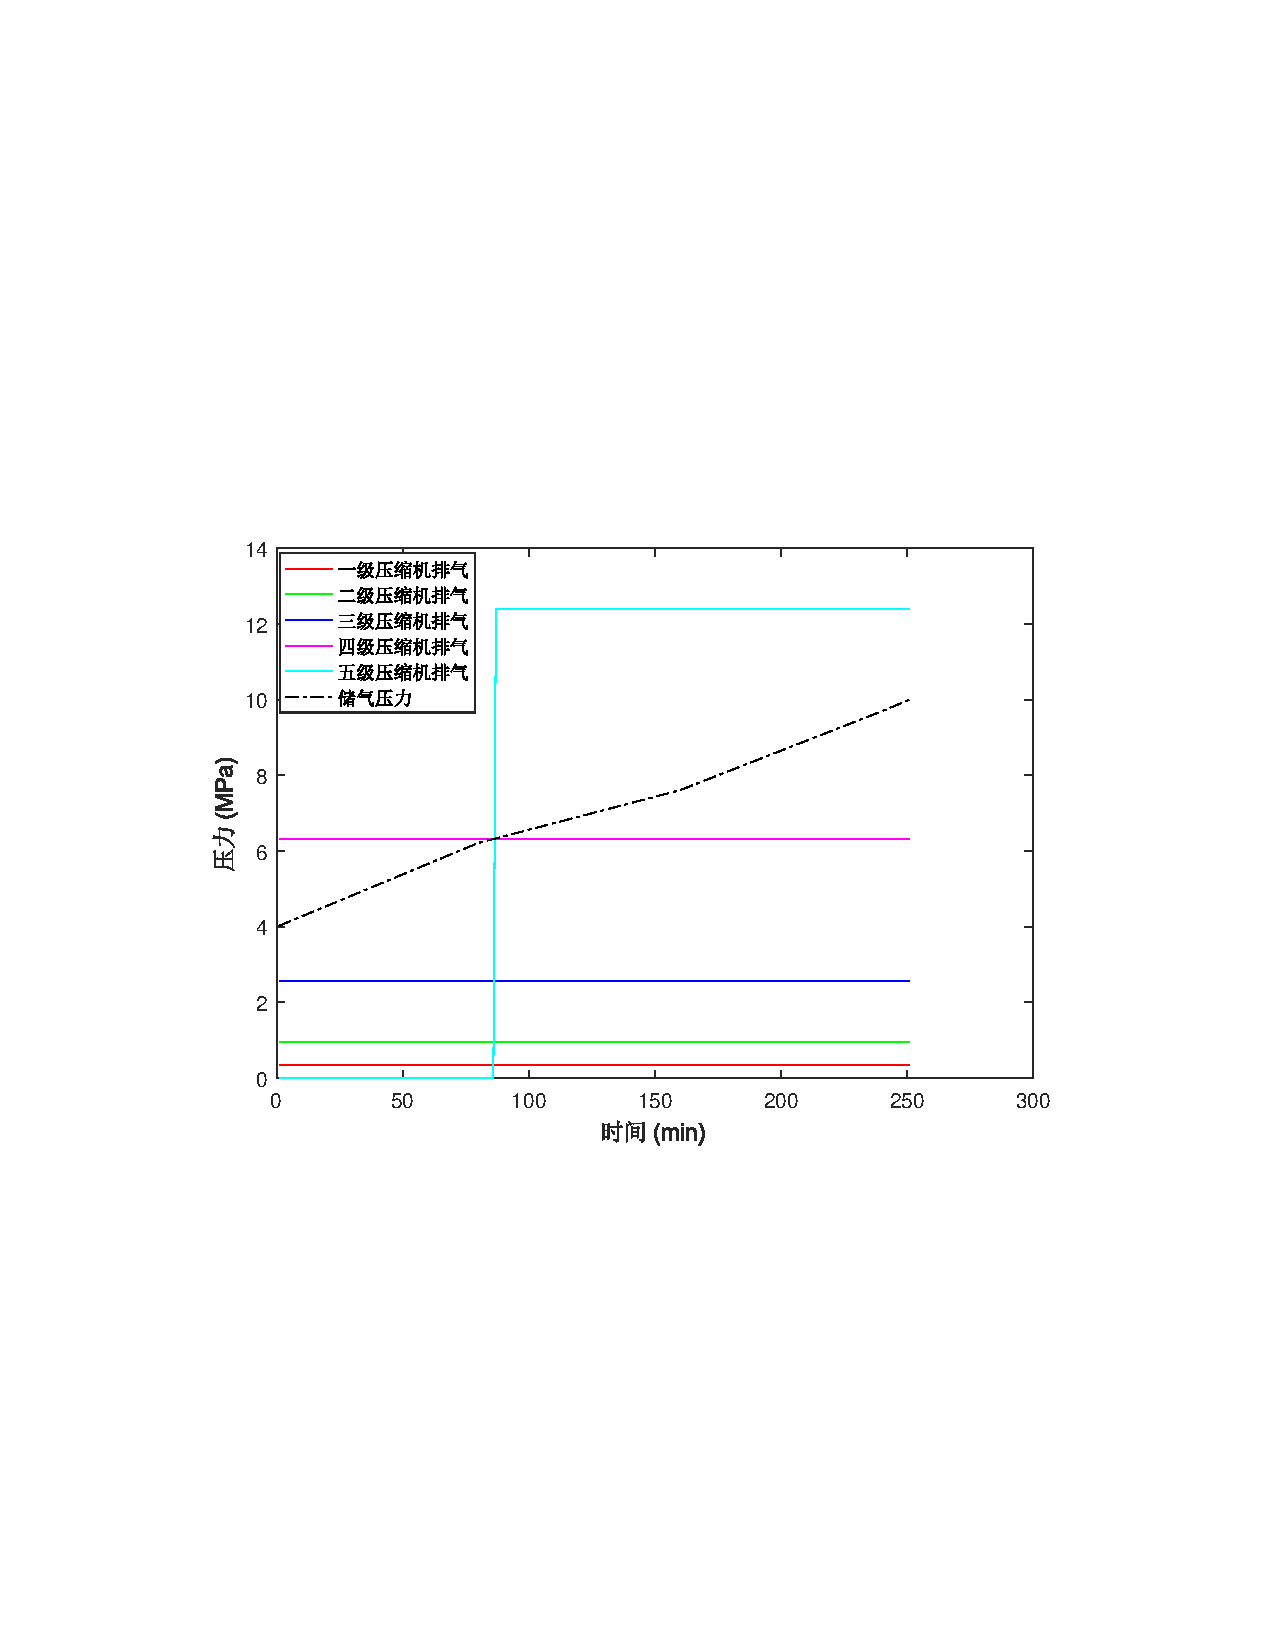
\includegraphics[scale=0.70]{Chap2-Sim-Char-Inlet-Pressure-Part-load.pdf}
  \caption{压缩储能过程压缩机入口压力变化曲线(部分负载)}
  \label{fig:Sim-Char-Inlet-Pressure-Part-load}
\end{figure}

由图\ref{fig:Sim-Char-Inlet-Pressure-Part-load}可知,储气库储气压力的变化趋势与质量流率的变化趋势一致,可近似分为三段,第一段为从0min-80min, 第二段为从81min-160min,第三段为160min-250min,相应的储气库内空气温度及空气总质量也存在同样的趋势。

\begin{figure}[H] % use float package if you want it here
  \centering
  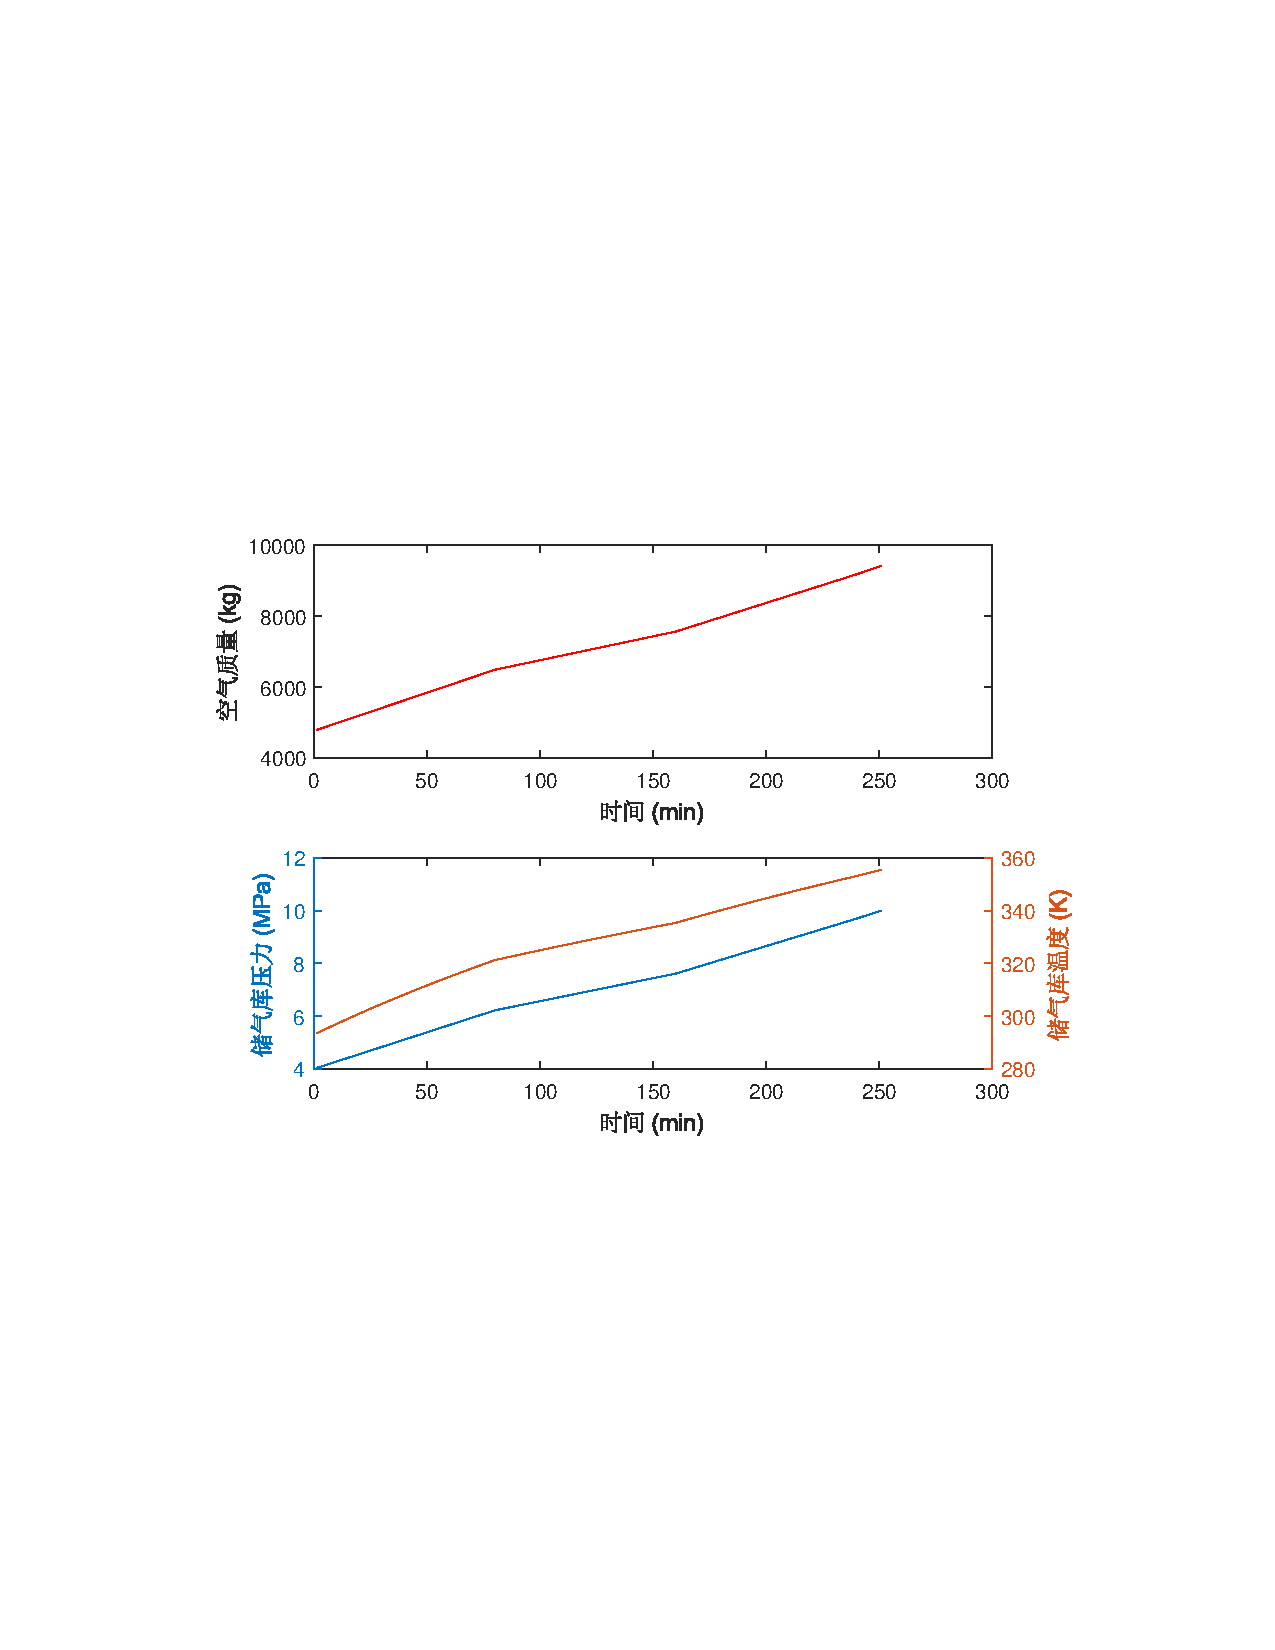
\includegraphics[scale=0.76]{Chap2-Sim-Char-ASU-Part-load.pdf}
  \caption{压缩储能过程储气库动态特性(部分负载)}
  \label{fig:Sim-Char-ASU-Part-load}
\end{figure}

图\ref{fig:Sim-Char-Heat-Quan-Part-load}给出了各级换热器换热功率的变化曲线。尽管换热器量变换趋势与质量流率趋势一致,但由于以部分负载模式运行时换热器等熵效率的降低,导致整个储热过程存储的高温HTF的降低,如图\ref{fig:Sim-Char-TES-Part-load}所示。

\begin{figure}[H] % use float package if you want it here
  \centering
  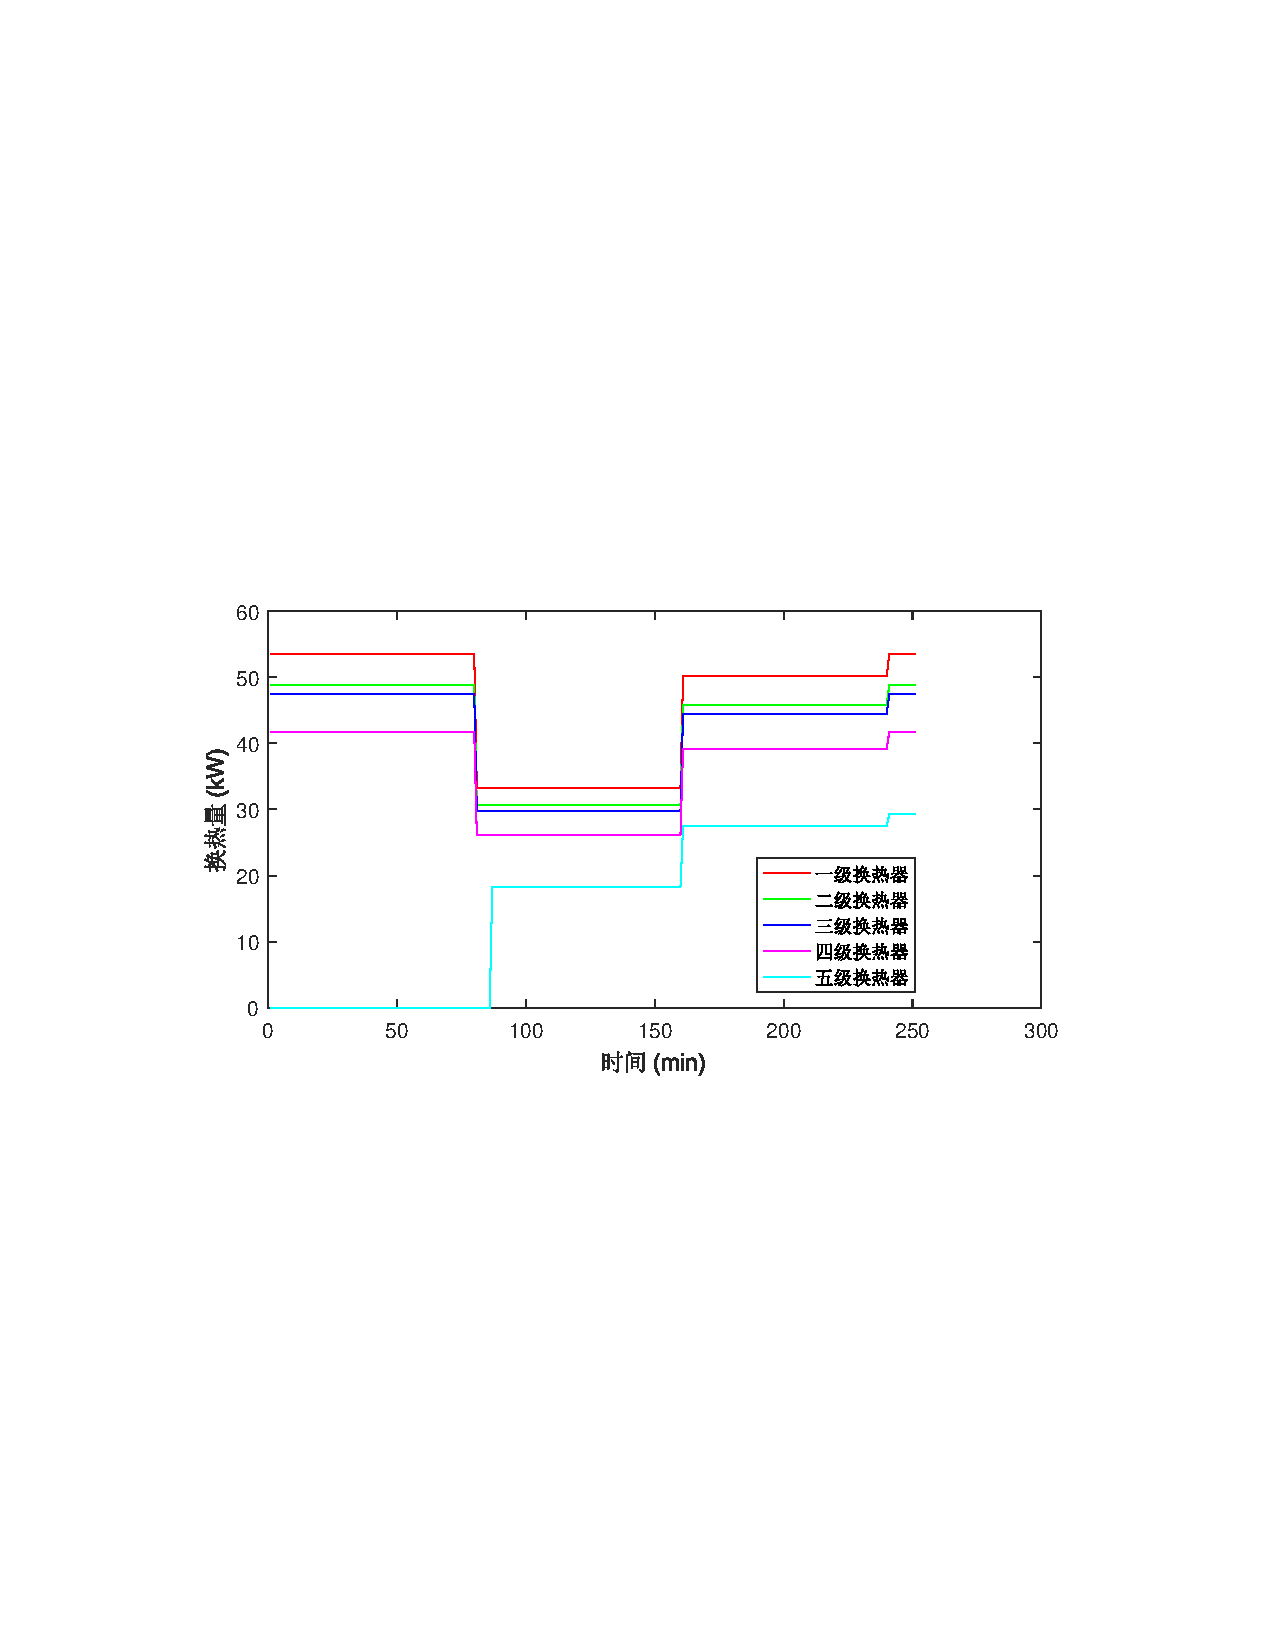
\includegraphics[scale=0.70]{Chap2-Sim-Char-Heat-Quan-Part-load.pdf}
  \caption{压缩储能过程换热器换热量变化曲线(部分负载)}
  \label{fig:Sim-Char-Heat-Quan-Part-load}
\end{figure}

压缩储能结束时储热罐中存储的储热介质质量由设计工况下的7.0973$\times 10^3$kg降为7.0407$\times 10^3$kg。与设计工况类似,由于在压缩侧滑压运行过程中第5级压缩机的启动,储热罐中HTF的温度在压缩储能过程的后期也有所降低。但是,由于在部分负载运行模式下流经换热器的HTF的质量流率相应减小,导致压缩储能结束时储热罐中HTF的温度(400.35K)稍高于设计工况(400.27K)。

\begin{figure}[H] % use float package if you want it here
  \centering
  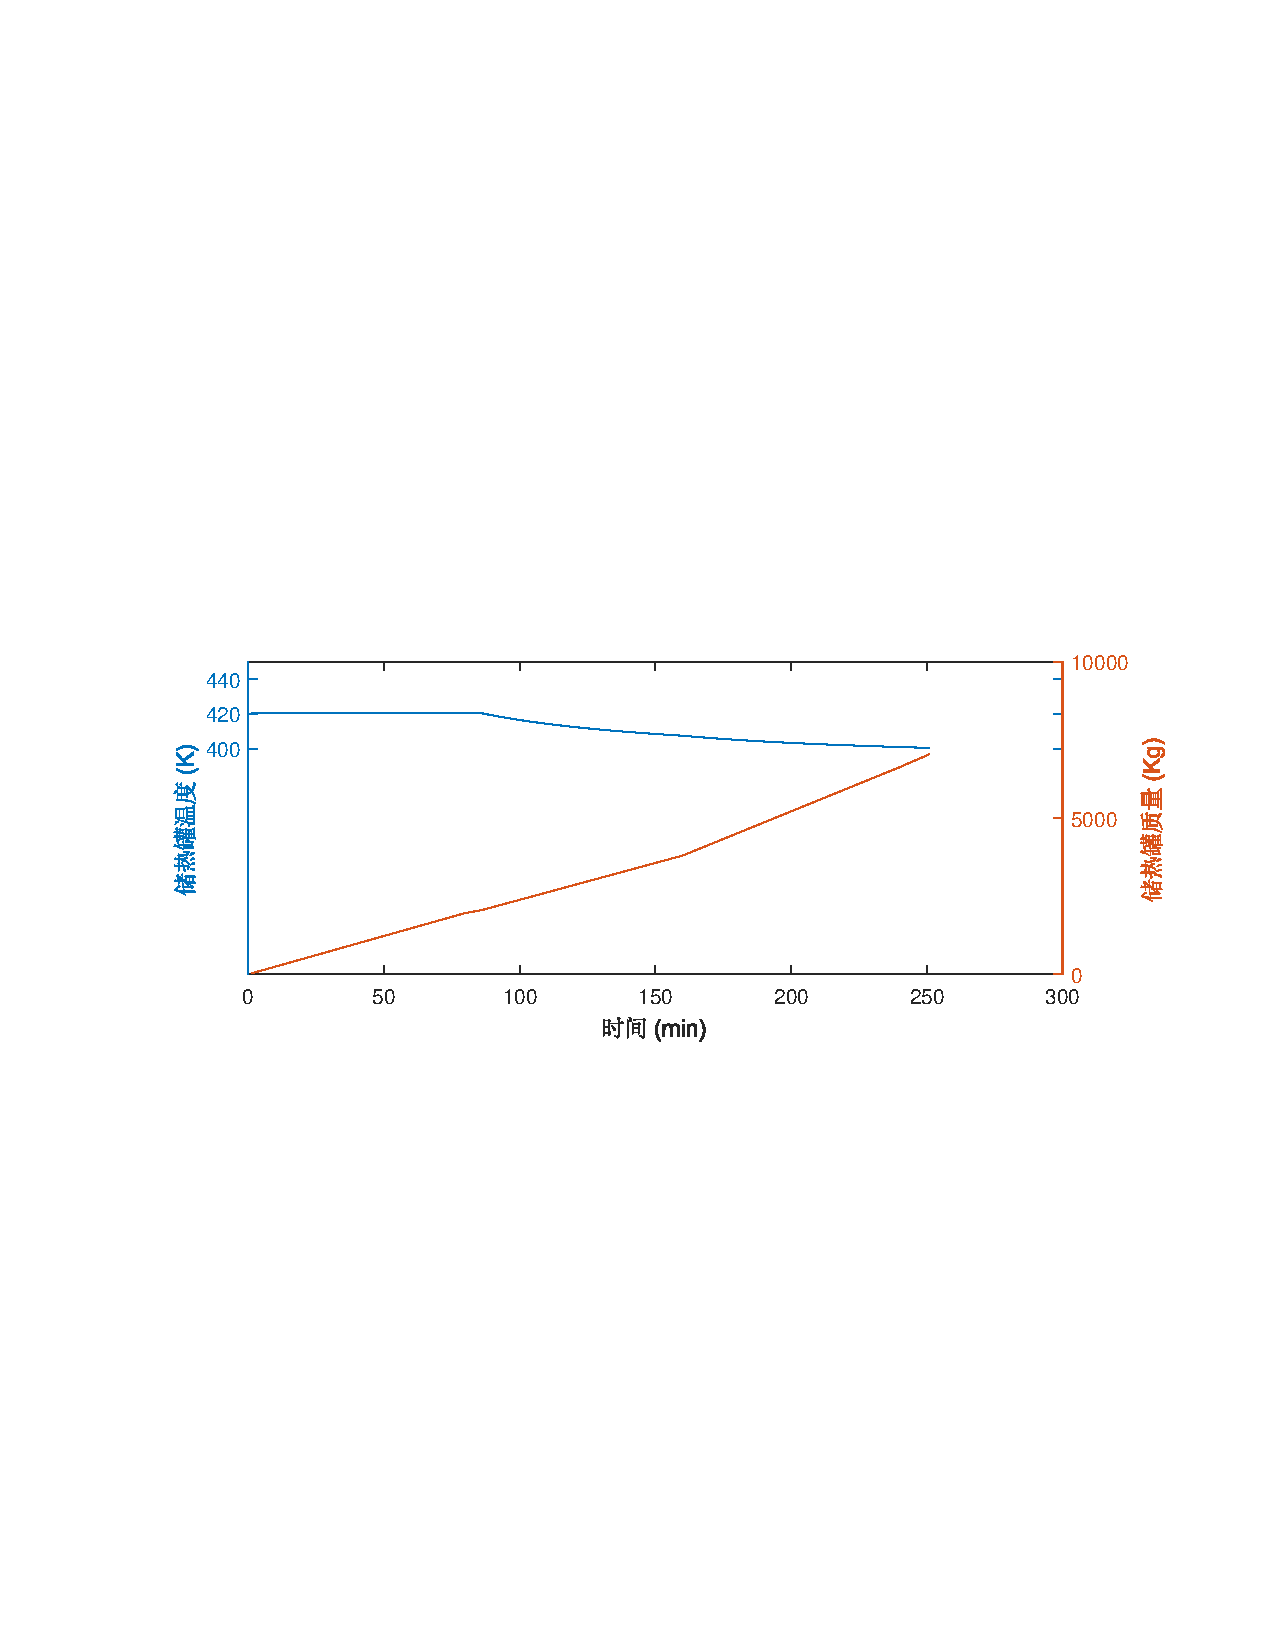
\includegraphics[scale=0.70]{Chap2-Sim-Char-TES-Part-load.pdf}
  \caption{压缩储能过程储热罐动态特性(部分负载)}
  \label{fig:Sim-Char-TES-Part-load}
\end{figure}

图\ref{fig:Sim-Char-Comp-Power-Part-load}给出了部分负载模式下压缩过程中各级压缩级的耗功。可以得出,质量流率的调节在一定程度上实现了压缩侧耗功功率的调节。在第5级压缩机未启动之前,在第81min由于压缩侧质量流率的突然减小(见图\ref{fig:Sim-massflow-Part-load}),导致压缩侧总耗功的突变,在第85min随着压缩侧背压升高,第5级压缩机启动后,压缩侧耗功回升。

\begin{figure}[H] % use float package if you want it here
  \centering
  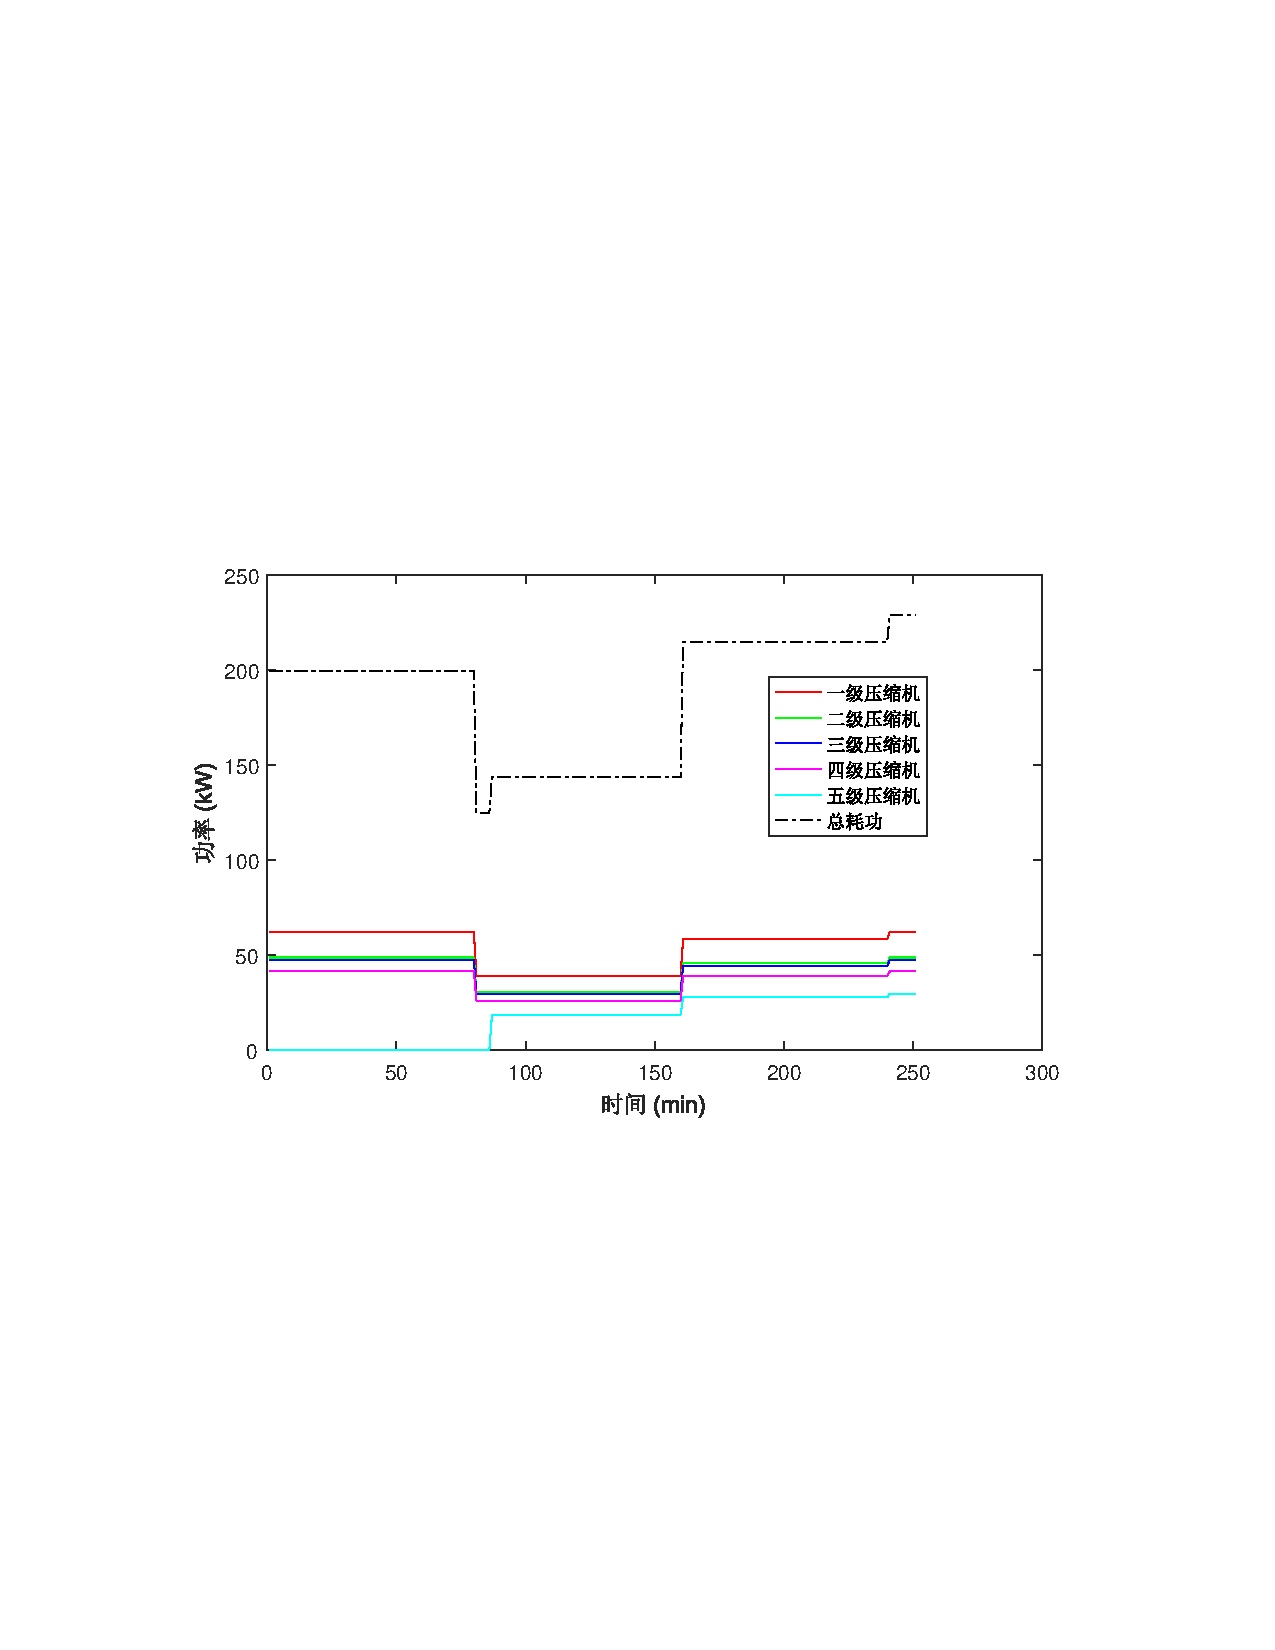
\includegraphics[scale=0.70]{Chap2-Sim-Char-Comp-Power-Part-load.pdf}
  \caption{压缩储能过程压缩机耗功变化曲线(部分负载)}
  \label{fig:Sim-Char-Comp-Power-Part-load}
\end{figure}

\subsubsection{膨胀释能过程}
在膨胀侧的常压释能过程中,按部分负载模式质量流率放气的总时间为0.78h,图\ref{fig:Sim-Disc-ASU-Pressure-Part-load}给出了整个释能过程中各级透平进气压力及储气库内空气压力的变化曲线。尽管储气库内空气压力一直在降低,但由于储气库出口侧节流阀的“稳压”作用,各级透平的进气压力均可维持核定,从而改善了由于压力偏离设计值造成的透平的部分负载运行特性。

%\subsection{适用性讨论}
\begin{figure}[H] % use float package if you want it here
  \centering
  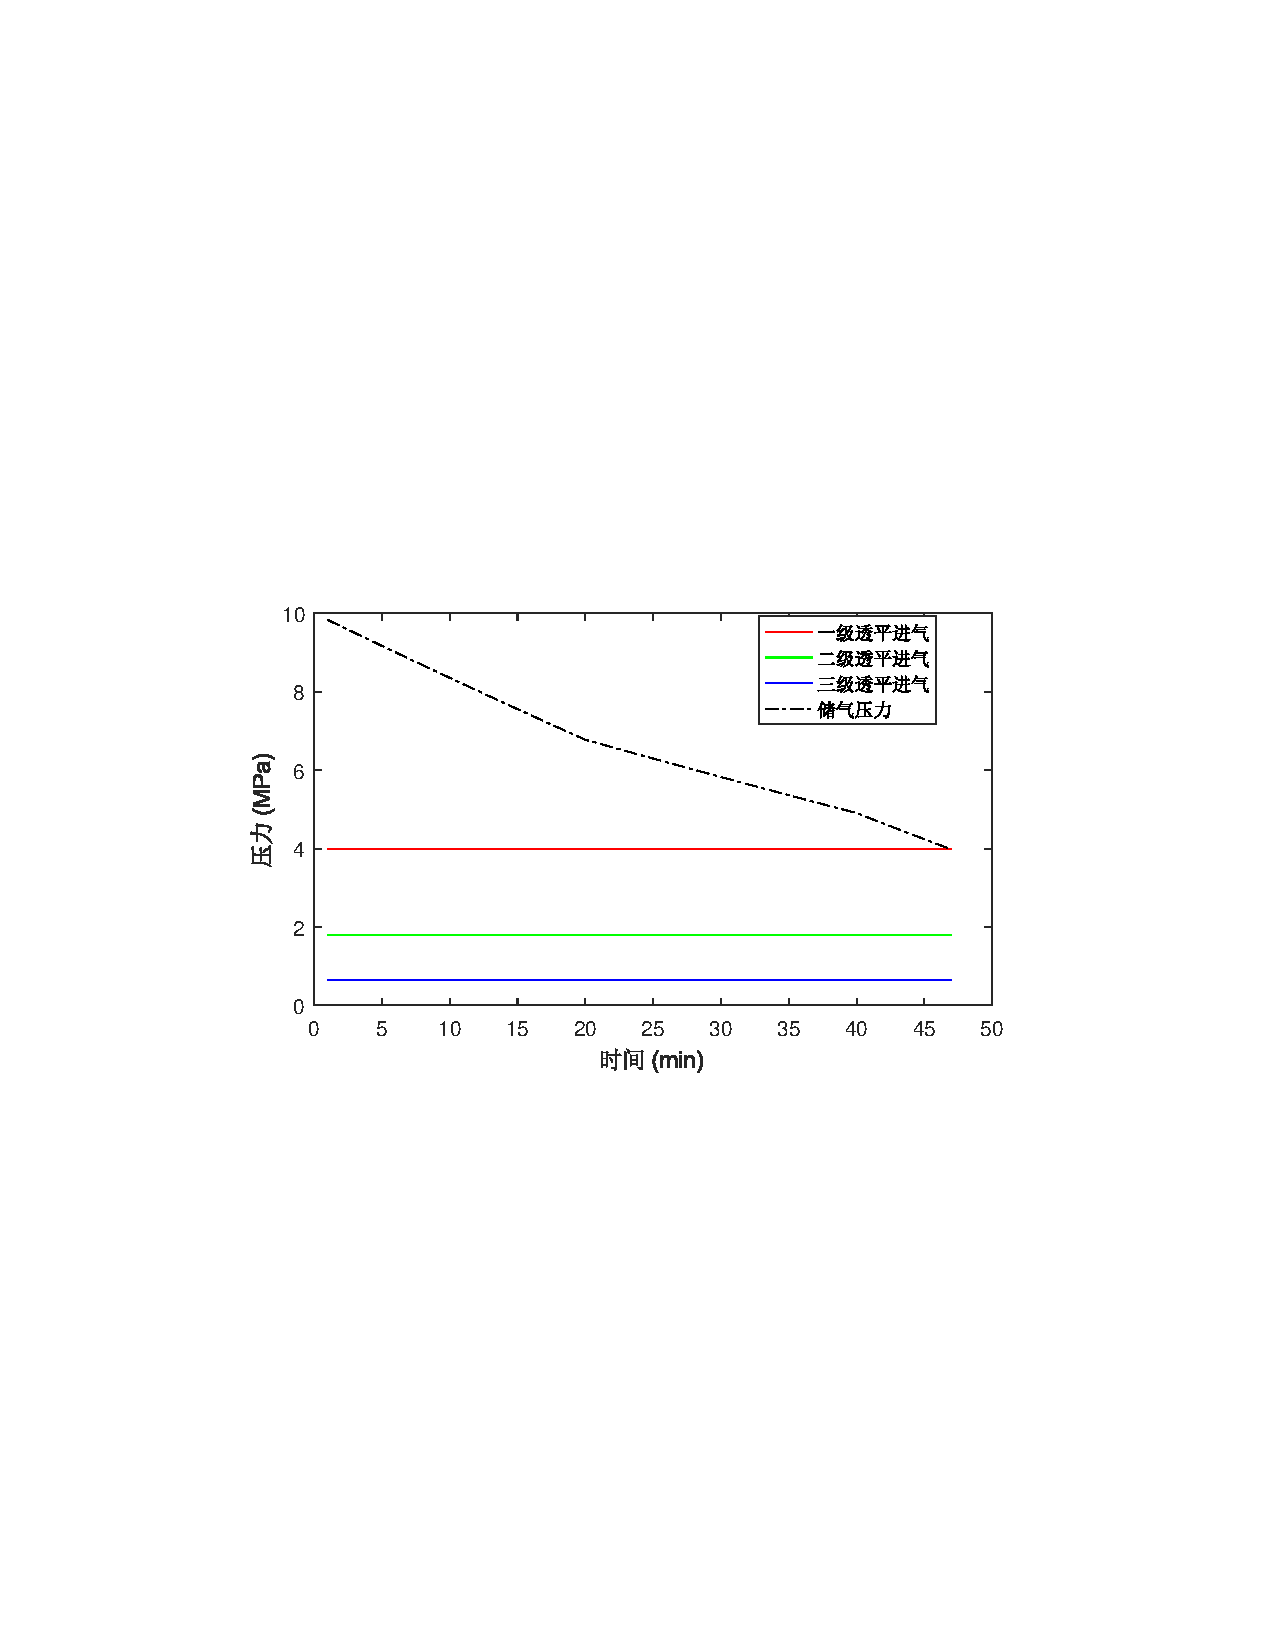
\includegraphics[scale=0.82]{Chap2-Sim-Disc-ASU-Pressure-Part-load.pdf}
  \caption{膨胀释能过程储气库动态特性(部分负载)}
  \label{fig:Sim-Disc-ASU-Pressure-Part-load}
\end{figure}

图\ref{fig:Sim-Disc-Heat-Quan-Part-load}给出了各级换热器换热功率的变化趋势。在部分负载模式下,受储气库内空气温度的变化(类似于设计工况)以及放气质量流率变化的综合影响,换热器的换热功率表现出较为复杂的特性。例如,在0-20min的释能阶段,储气库内空气温度的变化对换热器换热需求的影响占主导作用,储气库温度的降低,增加了各级换热器换热功率的需求;在第20min由于放气质量流率的降低幅度较大(见图\ref{fig:Sim-massflow-Part-load}),降低了换热器整体的换热功率需求;随着空气侧质量流率的固定,储气库温度变化对各级换热器换热的影响占主导。

\begin{figure}[H] % use float package if you want it here
  \centering
  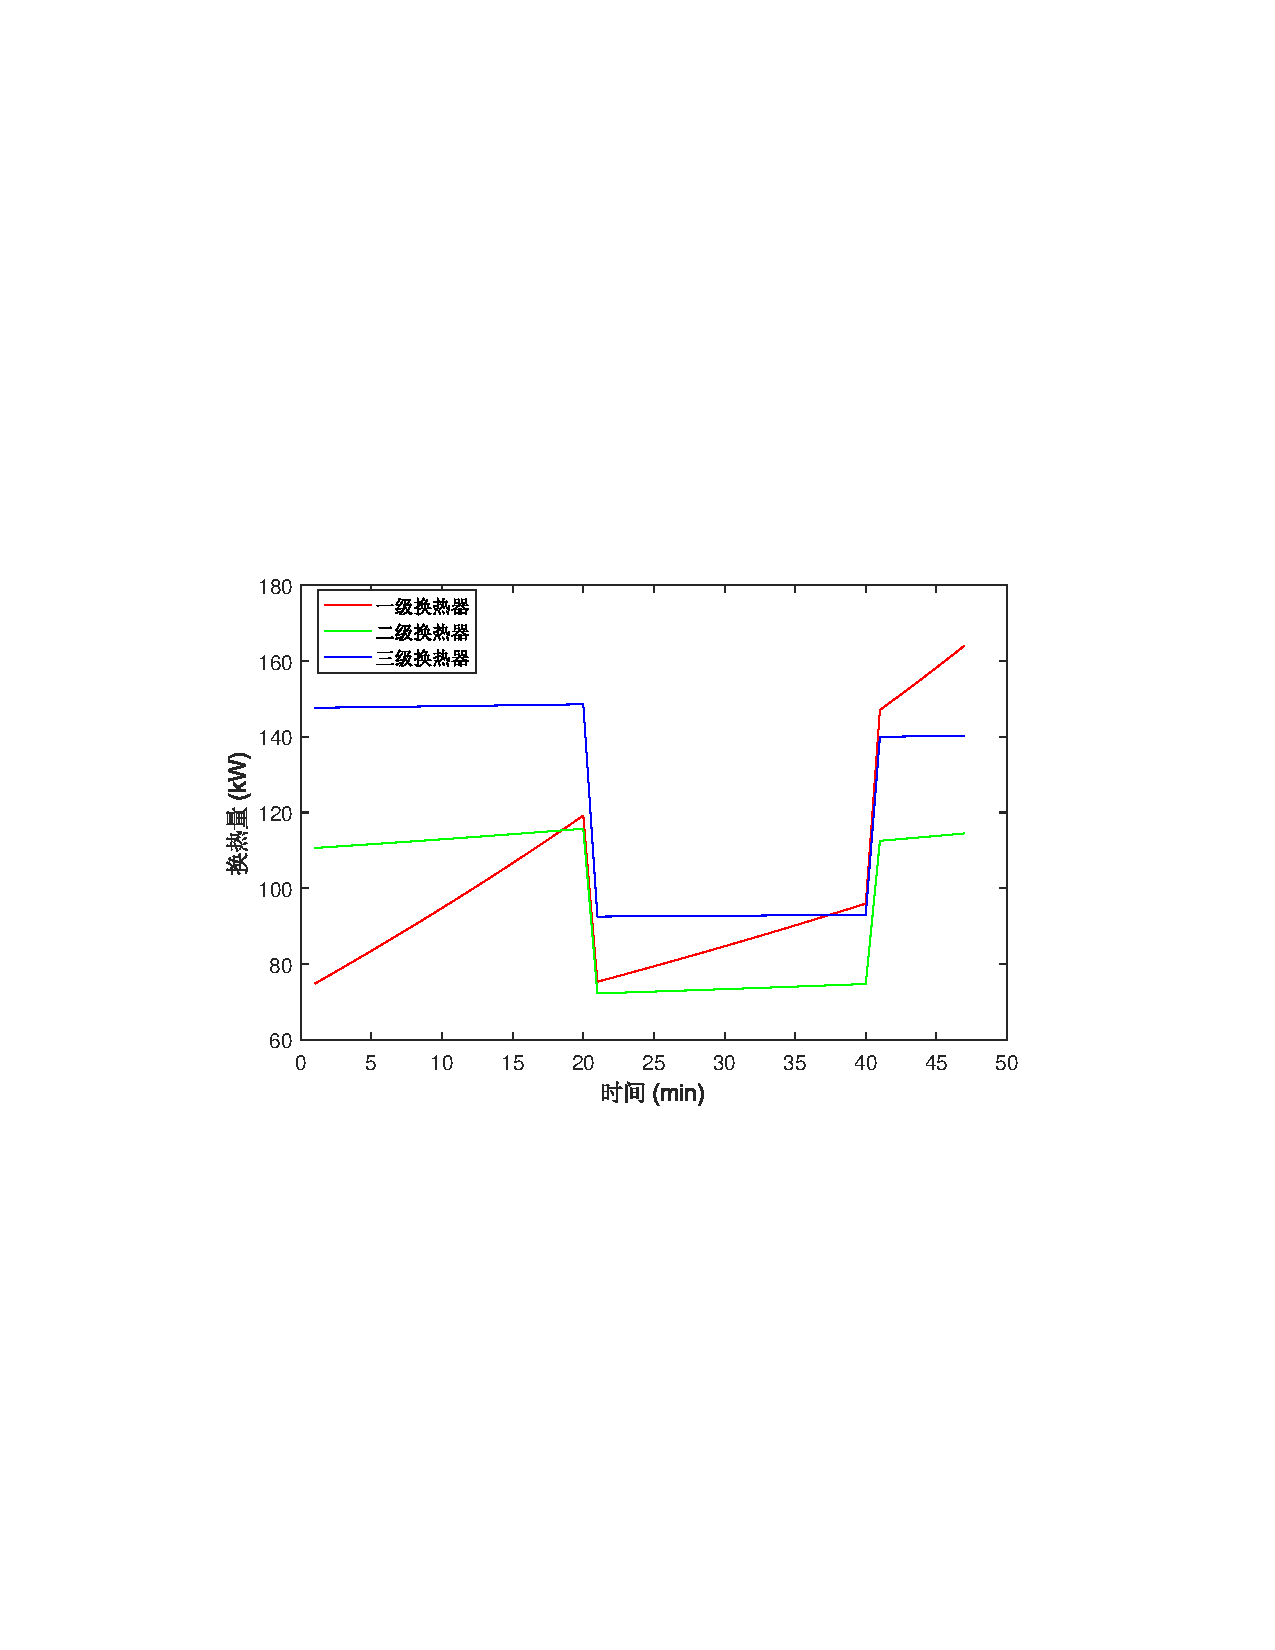
\includegraphics[scale=0.77]{Chap2-Sim-Disc-Heat-Quan-Part-load.pdf}
  \caption{膨胀释能过程换热器换热功率(部分负载)}
  \label{fig:Sim-Disc-Heat-Quan-Part-load}
\end{figure}

图\ref{fig:Sim-Disc-Turb-Power-Part-load}给出了部分负载模式下,各级透平及AA-CAES的总输出功率。由于质量流率偏离设计值,降低了释能环节透平的实际运行等熵效率,从而降低了系统输出功率。

\begin{figure}[H] % use float package if you want it here
  \centering
  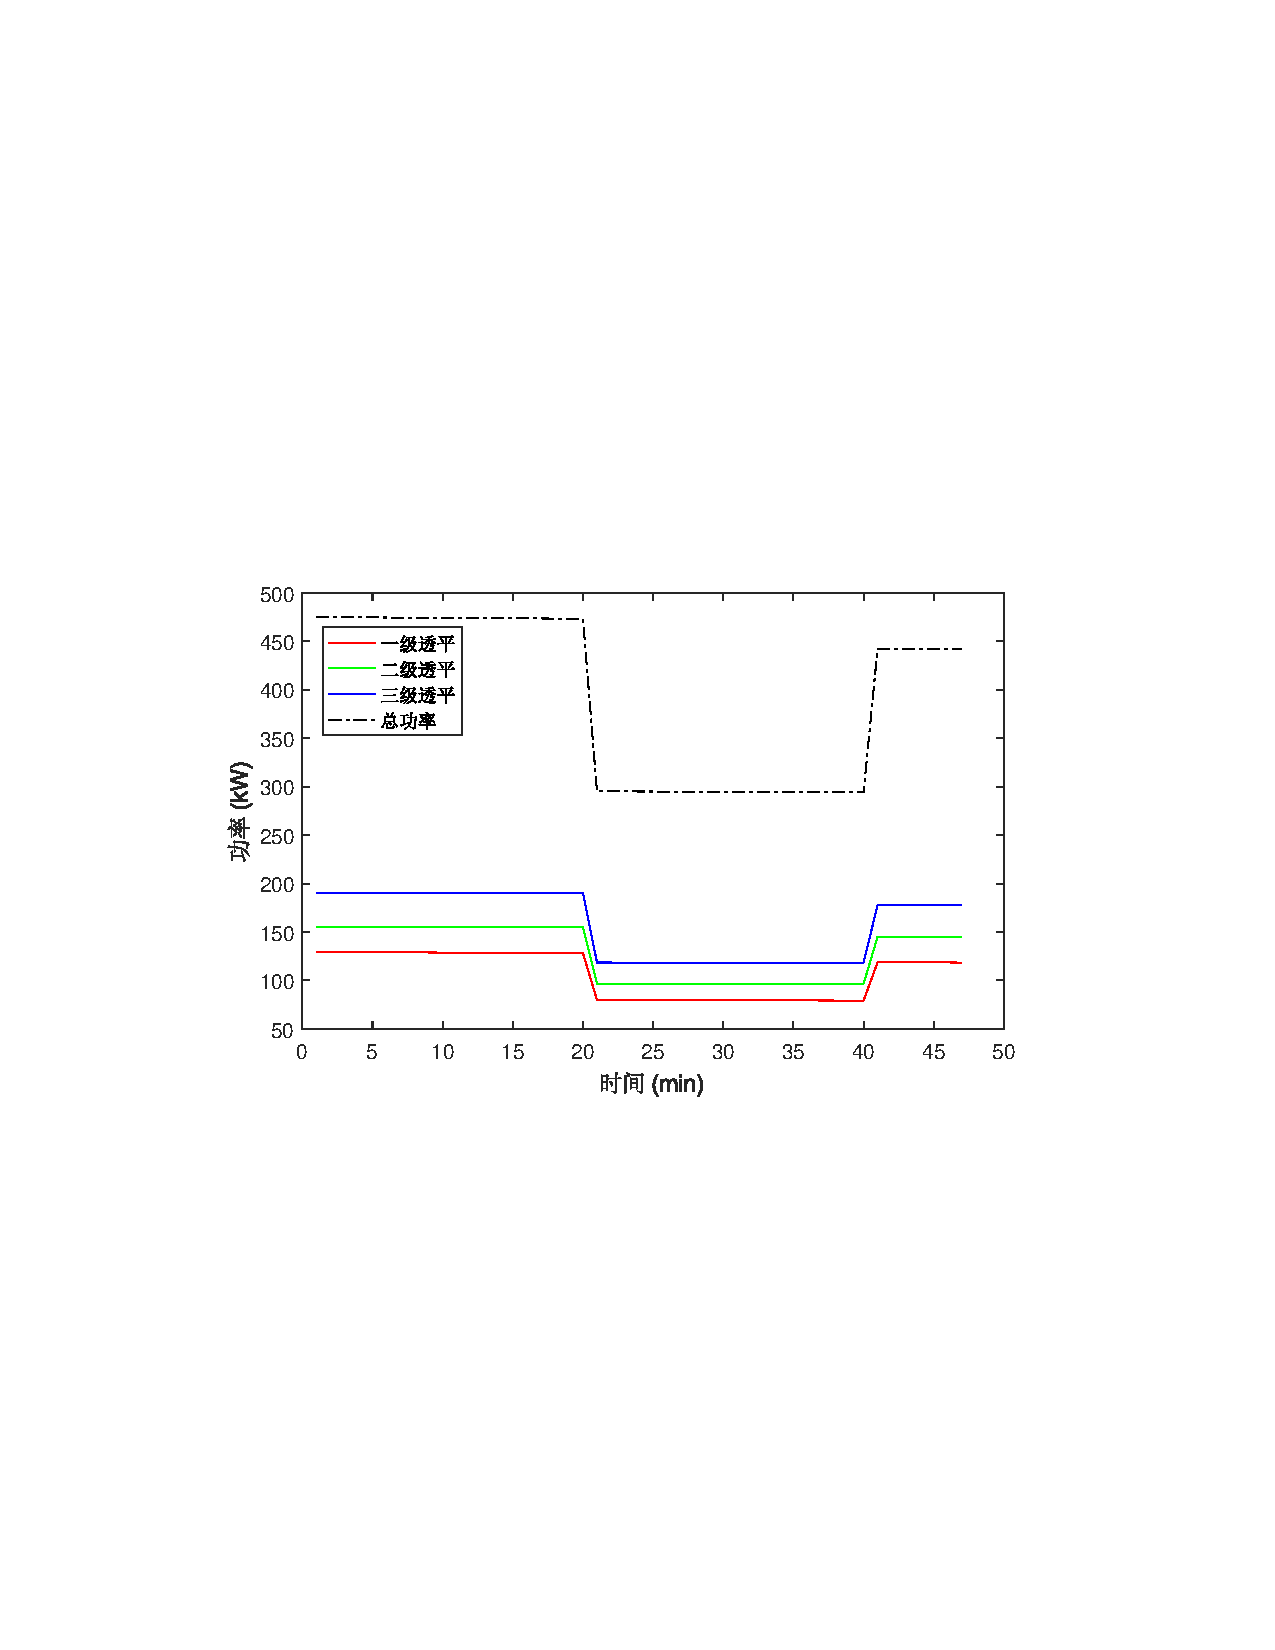
\includegraphics[scale=0.80]{Chap2-Sim-Disc-Turb-Power-Part-load.pdf}
  \caption{膨胀释能过程输出功率变化曲线(部分负载)}
  \label{fig:Sim-Disc-Turb-Power-Part-load}
\end{figure}

综上,以本节给定的部分负载质量流率进行压缩储能与膨胀释能的一个循环周期中,AA-CAES消耗的总电量为0.8259MWh,输出的总电量为0.3079MWh,其电-电效率$\eta_{elec}$ 为37.28\%,与设计工况相比相对下降6.87\%。储能结束时高温储热罐中的HTF质量为7.0407$\times10^3$kg,释能结束时储热罐中剩余的HTF质量为3.3266$\times10^3$kg,温度为400.35K,可用于供热的热量为0.3563MW,供热效率为$\eta_{heat}$为43.14\%,系统热电热联供的总能利用系数$\eta_{total}$为80.42\%。供热的热量㶲为0.0955MWh,供热㶲效率为11.56\%,总㶲效率为48.58\%。对比设计工况与宽工况算例可知,部分负载运行模式降低了系统的电-电效率、总能利用系数以及总㶲效率。需要说明的是,在本节的仿真中我们采用了小容量的AA-CAES系统,其储气与储热系统均能实现绝热,若考虑储气库及储热系统的传热损失,则上述分析中的效率指标均会有所下降。

\section{小结}
实现面向宽工况应用的AA-CAES准确的组件级部分负载热力学特性建模与分析是研究AA-CAES运行模型及市场运营策略等的前提。本章结合新能源电力系统中AA-CAES的典型应用场景对其宽工况运行的要求,以及由此导致的内部组件级别的部分负载特性,建立了AA-CAES通用宽工况热力学稳态仿真模型。同时,基于构建的热力学仿真模型分析了一典型AA-CAES试验系统在多种运行模式及多种供能模式下的运行特性,为源-网-荷侧相应AA-CAES实现形式的建模与分析提供了基础。
